\documentclass[a4paper,brazil,ruledheader,normaltoc,capchap,twoside,openany]{include/abnt}
\usepackage[a4paper,left=3cm,right=2cm,top=3cm,bottom=2cm]{geometry}
\usepackage{newclude}
\usepackage{pdflscape}
\usepackage[T1]{fontenc}
\usepackage{ae} 
\usepackage[utf8x]{inputenc}
\usepackage[printonlyused]{include/acronym}
\usepackage{multirow}
\usepackage[alf,no-abnt-option-file]{include/abntcite}
\renewcommand{\emph}{\textsc}
\usepackage{multibib}
\usepackage[brazil]{babel}
\usepackage{include/abnt-PPGInf-PUCMG}
\usepackage[pdftex]{graphicx}
\usepackage{epstopdf}
\usepackage{float}
\usepackage[symbol]{footmisc}
\usepackage[all]{xy}
\usepackage{url}
\usepackage{amsthm}
\usepackage{amsmath}
\usepackage{amssymb}
\usepackage[portuguese,linesnumbered,ruled,vlined]{algorithm2e}
\usepackage{algorithmic}
\usepackage{listings}
\setlength{\algomargin}{1em}
\usepackage{setspace}
\usepackage{rotating}
\usepackage{pstricks}
\usepackage{color}
\usepackage{array}
\usepackage{tabularx}
\usepackage{longtable}
\usepackage{colortbl}
\usepackage{ifthen}
\usepackage[size=normalsize,labelfont=bf,textfont={bf},labelsep=endash]{caption}
\captionsetup[subfloat]{labelfont=bf,textfont={bf}}
\usepackage{paralist}
\usepackage[none]{hyphenat} % O texto não usará hifenização com esse pacote
\usepackage{placeins}
%\usepackage{adjustbox}
%\usepackage{pdfpages}
\usepackage{silence}
\WarningFilter{caption}{Unsupported}
\WarningFilter{caption}{Unused}
\WarningsOff

\usepackage{pdfpages}
\usepackage{comment}
%Pacote para utilizar notas no texto. Para a versão final, basta passar o parâmetro "disable" no \todo[] que o PDF será criado sem as notas.
\usepackage[textwidth=1.7cm]{todonotes}
\setlength{\marginparwidth}{1.6cm}
\newcounter{todocounter}
%\newcommand{\smalltodo}[2][]
%{\todo[caption={#2}, #1]
%{\begin{spacing}{0.5}#2\end{spacing}}}
\newcommand{\note}[2][]
%COMANDO PARA AS NOTAS APARECEREM NA MARGEM DO TEXTO
%{\todo[caption={#2}, size=\tiny, #1,color=green!40]{\renewcommand{\baselinestretch}{0.5}\thetodocounter: #2\par}}
%COMANDO PARA AS NOTAS APARECEREM NO CORPO DO TEXTO
{\stepcounter{todocounter}\todo[caption={#2}, size=\small, inline, #1,color=green!40]{\renewcommand{\baselinestretch}{0.5}\thetodocounter: #2\par}}
%{\stepcounter{todocounter}\todo[caption={#2}, size=\small, inline, #1,color=green!40,disable]{\renewcommand{\baselinestretch}{0.5}\thetodocounter: #2\par}}

%\usepackage{xcolor}
%\newcommand\note[1]{\textcolor{red}{#1}}
%\renewcommand\note[1]{}
%\newcommand

%\usepackage[draft]{changes}
%\usepackage[final]{changes}
%\definechangesauthor[color=blue]{Pedro}
%\definechangesauthor[color=red]{Mark}
%%% Alternative definition to have the remarks
%%% in the margins instead of footnotes
%\usepackage[textwidth=1.7cm]{todonotes}
%\setlength{\marginparwidth}{1.7cm}
%\makeatletter
%\setremarkmarkup{\todo[color=Changes@Color#1!20,size=\tiny]{#1: #2}}
%\makeatother
%% Rather hacky definition of a plain remark/note
%% by riding on \added
%\newcommand{\note}[2][]{\added[#1,remark={#2}]{}}


\captionsetup{figurewithin=none}
\captionsetup{tablewithin=none}
\setlength{\LTcapwidth}{\textwidth}
\setcounter{tocdepth}{3}
\setcounter{secnumdepth}{3}


%\floatstyle{plaintop}
%\newfloat{grafico}{H}{loq}
%\restylefloat*{grafico}
%\floatname{grafico}{Gráfico}

\usepackage{subfig}
%\newsubfloat[position=bottom,listofformat=subsimple]{grafico}
\newsavebox{\leftfig}
\newsavebox{\rightfig}

\floatstyle{plaintop}
\newfloat{quadro}
\restylefloat{quadro}
\floatname{quadro}{Quadro} 

\makeatletter
%\renewcommand{\ALG@name}{Algoritmo}
%\renewcommand{\listalgorithmname}{Lista de Algoritmos}

\lstset{extendedchars=\true, % permite acentos
 inputencoding=utf8x,
 literate={\$}{{\$}}1,
 commentstyle=\it, % deixa os comentários em itálico
 stringstyle=\bf, % não lembro o que faz, mas está funcionando
 belowcaptionskip=5pt, % não lembro o que faz, mas está funcionando
 numbers=left, % coloca a numeração na esquerda
 stepnumber=1, % passos da numeração
 firstnumber=1, % primeira linha
 numberstyle=\tiny, % tamanho da fonte da numeração
 breaklines=true, % permitir quebra de linha
 frame=tb, % borda em cima e em baixo
 basicstyle=\footnotesize, % estilo básico
 stringstyle=\ttfamily, % não lembro o que faz, mas está funcionando
 showstringspaces=false, % não mostrar os espaços
 mathescape, % não lembro o que faz, mas está funcionando
 tabsize=3 % tamanho da tabulação
}
\renewcommand{\lstlistingname}{Código}
\renewcommand{\lstlistlistingname}{Lista de Códigos}
\citeoption{abnt-etal-cite=1, abnt-and-type=e}

\renewcommand{\thefootnote}{\arabic{footnote}}

\graphicspath{{./imagens/}}

\begin{document}
\sloppy
% Para forçar que elementos pré-textuais (da capa até o sumário) sejam impressos no anverso da folha
\setboolean{@twoside}{false}

\autor{Ericson Marquiere Reis Silva}

\titulo{\uppercase{Cart-OnePiece - A Tool for Dataset Generation, Workload Characterization, and Task Scheduling Benchmarking for Autonomous Driving Vehicles}}

\orientador[Advisor:]{Prof. Dr. Henrique Cota de Freitas}
%\coorientador[Co-orientadora:]{Profa. Dra. Ana Maria Pereira Cardoso}

%\area{Ciência da Computação}

\comentario{Thesis proposal presented to the Graduate Program in Informatics at the Pontifícia Universidade Católica de Minas Gerais, as a partial requirement to obtain the qualification of
the title of Doctor in Informatics.}

\instituicao{Doutorado em Informática \par Instituto de Informática \par Pontifícia Universidade Católica de Minas Gerais}

\local{Belo Horizonte}

\data{2024}

\capa

% Para forçar que a ficha catalográfica seja impressa no verso da folha de aprovação
\setboolean{@twoside}{true}

\folhaderosto

%% Ficha catalográfica
% INCLUIR O ARQUIVO PDF GERADO PELA BIBLIOTECA COMO FIGURA.
\begin{figure}[!ht]
	\vspace*{-3.3cm}
%	% Suponha o nome do arquivo em pre-texto/ficha-catalografica/fichacatalografica.pdf
	\hspace*{-3cm}
	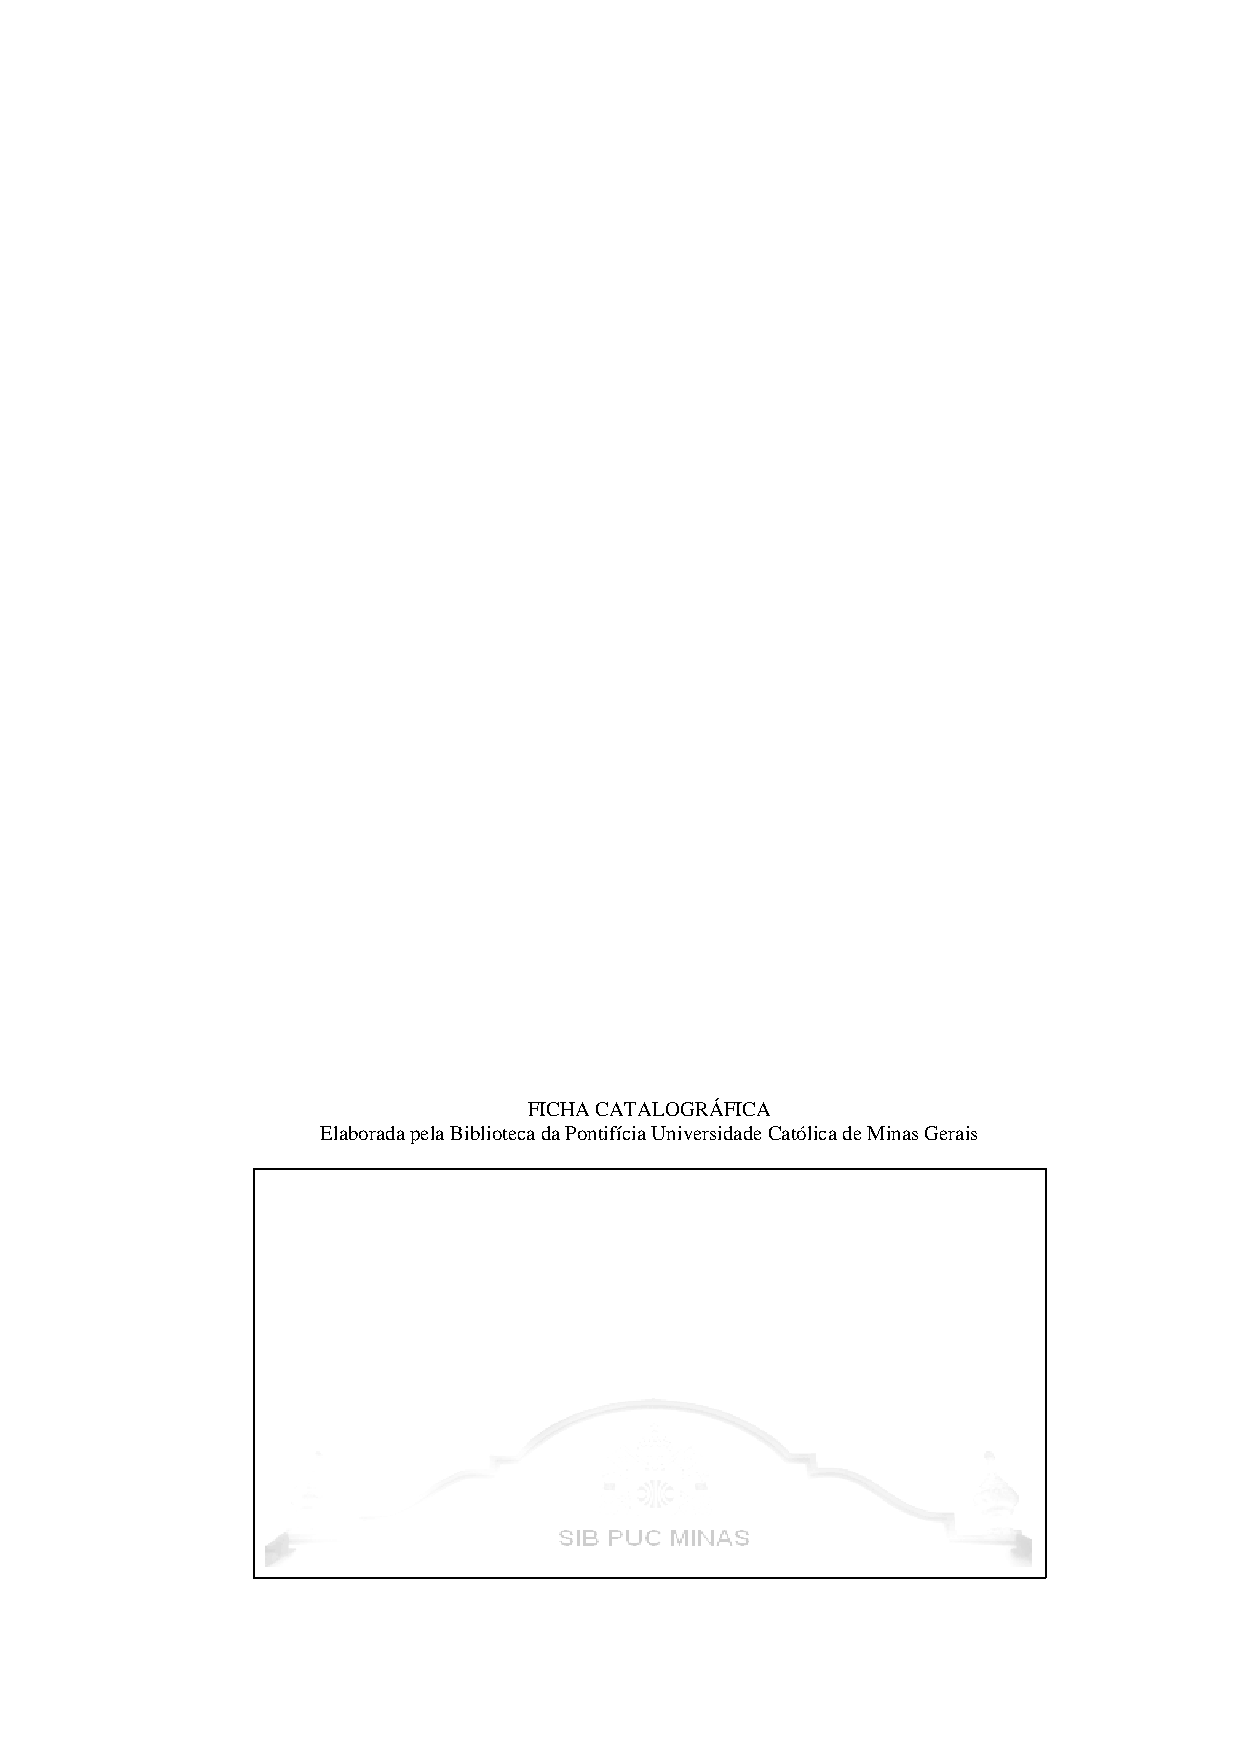
\includegraphics{pre-texto/ficha-catalografica} 
	\newpage
\end{figure}

% Para forçar que elementos pré-textuais (da capa até o sumário) sejam impressos no anverso da folha
\setboolean{@twoside}{false}

%% Termo de Aprovação

% Texto da aprovação
\textoaprovacao{Proposta de tese apresentado ao Programa de Pós-Graduação em Informática da Pontifícia Universidade Católica de Minas Gerais, como requisito de qualificação para o título de Doutor em Informática.}

\primeiroassina{
	Prof. Dr. Henrique Cota de Freitas -- PUC Minas (Orientadora)
}
\segundoassina{
	Prof. Dr. X -- PUC Minas (Banca Examinadora)
}
\terceiroassina{
	Prof. Dr. X -- PUC Minas (Banca Examinadora)
}
\quartoassina{
	Prof. Dr. X -- UFV (Banca Examinadora)
}
%\quintoassina{Profa. Dra. X -- UFV (Banca Examinadora)}


\localdia{Belo Horizonte, XX de Agosto de 2018}

\termodeaprovacao
%\include{pre-texto/dedicatoria}
%% Agradecimentos
%\chapter*{Agradecimentos}
\begin{center}
	\normalsize
	\textbf{AGRADECIMENTOS}
\end{center}

Agradecimentos....
 


%% Epígrafe
\newpage

% Espaçamento entre topo da página e texto da epígrafe
\vspace*{10cm}
% Espaçamento na esqueda
\hspace{4cm}\begin{minipage}{.51\textwidth}

% Texto da epígrafe
\textit{``Nós só podemos ver um pouco do futuro, mas o suficiente para perceber que há muito a fazer.'' }

%Nome do autor
\begin{flushright}\itshape Alan Turing \upshape\end{flushright}

\end{minipage}
%\begin{resumo}
\vspace{0.4cm}
\onehalfspacing

\noindent 
O aumento de desempenho de processadores é um desafio que cresce a cada dia, principalmente com as preocupações relacionadas à eficiência energética.
O uso de arquiteturas com nível de paralelismo cada vez maior para atender a alta demanda de processamento de dados é uma realidade, logo, processadores \textit{manycore} têm sido alvo de constantes propostas no que tange aos sistemas de interconexão em chip.
Algumas dessas plataformas \textit{manycore} consideram estratégias como agrupamentos de núcleos e redes-em-chip, que ofertam escalabilidade, possibilitando a inclusão de vários núcleos em um mesmo chip.

Por outro lado, há a necessidade de sistemas de memória suficientemente robustos para suportar o armazenamento para processamento do grande volume de dados.
Essa robustez do sistema de memória é fundamental para que os vários núcleos da arquitetura possam acessá-la, uma vez que problemas como contenção, latência de acesso e coerência podem ocorrer.
As arquiteturas \textit{manycore} tem contemplado sistemas de memória distribuídos, normalmente compartilhados entre um grupo de núcleos.
Esse modelo arquitetural resolve alguns dos problemas mencionados, mas outros permanecem, relacionados ao acesso justo à essas unidades distribuídas de memória, com o uso adequado da rede-em-chip, para os diversos núcleos.

Diante desses problemas, a presente proposta contempla o projeto de uma arquitetura parametrizável para controle de acesso justo às memórias em chip de processadores \textit{manycores}, que seja baseada em aprendizado de máquina.
Em linhas gerais, a arquitetura de controle tem um algoritmo de aprendizado de máquina implementado em hardware (e.g., K-Means ou Redes Neurais Artificiais), que recebe como dados de entrada informações do estado da arquitetura, e apresenta como saída sinais de controle para o sistema de memória e a rede-em-chip.
Tais sinais modificam, por exemplo, a estratégia de alocação de dados em memória e a estratégia de roteamento da rede-em-chip.
Para a construção do protótipo de arquitetura de controle proposta, uma exploração do espaço de projeto será realizada, em conjunto com ferramentas de desenvolvimento para simulação e descrição de hardware com foco em FPGA, considerando a presença do sistema de memórias distribuído e redes-em-chip, para aumentar o desempenho da arquitetura.

\vspace*{.50cm}
\noindent \textbf{Palavras-chave:} \textit{Manycores}. Redes-em-chip. Memória compartilhada e distribuída. Arquitetura parametrizável. FPGA. Aprendizado de máquina.\\
\end{resumo}
\begin{abstract}
\vspace{0.4cm}
\onehalfspacing

%\noindent 
The advancement of autonomous driving vehicles (ADVs) critically depends on efficient task scheduling within their heterogeneous processing systems to handle complex computational workloads in real time. Existing task scheduling methods, primarily designed for homogeneous or single-core systems, are inadequate for the multi-core, heterogeneous architectures of modern ADVs, leading to suboptimal performance and increased energy consumption.

To try to solve this challenge, this work proposes a novel smart task scheduling strategy employing reinforcement learning to optimize the allocation of computational tasks in ADVs. By modeling these tasks as a Directed Acyclic Graph, the proposed approach will try to learn optimal scheduling decisions based on real-time system metrics such as task execution times, resource requirements, dependencies, and current system load.

To evaluate the proposed strategy, an integrated test environment has been developed by combining the CARLA simulator with the StarPU runtime system, enabling the simulation of realistic ADV scenarios, such as the processing of sensor data and execution of perception algorithms in real time. This integration enabled the possibility of using StarPU's capability to define custom scheduling policies, allowing the reinforcement learning model to be smoothly incorporated into the scheduling framework and enabling direct control over task placement and resource allocation across ADV heterogeneous computing resources composed of CPUs and GPUs. 

Preliminary testing of existing scheduling strategies provided by StarPU has validated the feasibility of integration and provided insights into the performance characteristics of traditional scheduling algorithms in the simulated ADV environment.

\vspace*{.50cm}
\noindent Keywords: Autonomous Driving Vehicles. Heterogeneous Computing. Task Scheduling. Reinforcement Learning. \\
\end{abstract}


\makeatletter
\renewcommand\numberline[1]{
	\leftskip 0em
	\rightskip 1.6em
	\parfillskip -\rightskip
	\parindent 0em
	\@tempdima 2.0em
	\vspace{0em} \advance\leftskip \@tempdima \null\nobreak\hskip -\leftskip
	FIGURA \normalfont #1 -- }
\makeatother

% Lista de figuras
 \listoffigures
% \clearpage

\makeatletter
\renewcommand\numberline[1]{
	\leftskip 0em
	\rightskip 1.6em
	\parfillskip -\rightskip
	\parindent 0em
	\@tempdima 2.0em
	\vspace{0em} \advance\leftskip \@tempdima \null\nobreak\hskip -\leftskip
	TABELA \normalfont #1 -- }
\makeatother

% \listoftables
% \clearpage

\makeatletter
\renewcommand\numberline[1]{
	\leftskip 2em
	\rightskip 1.6em
	\let\belowcaptionskip\abovecaptionskip
	%\parfillskip -\rightskip
	\parindent 0em
	\@tempdima 2.0em
	\vspace{-3em} \advance\leftskip \@tempdima \null\nobreak\hskip -\leftskip
	QUADRO \normalfont #1 -- }
\makeatother

% \listof{quadro}{Lista de Quadros}
% \clearpage

%\makeatletter
%\renewcommand\numberline[1]{
%	\leftskip 0em
%	\rightskip 1.6em
%	\let\belowcaptionskip\abovecaptionskip
%	\parfillskip -\rightskip
%	\parindent 0em
%	\@tempdima 2.0em
%	\vspace{-3em} \advance\leftskip \@tempdima \null\nobreak\hskip -\leftskip
%	GRÁFICO \normalfont #1 -- }
%\makeatother

% Lista de graficos
%\listof{grafico}{Lista de Gráficos}

%% Lista de Abreviaturas e Siglas
%\chapter*{Lista de Abreviaturas e Siglas}
\chapter*{Lista de Abreviaturas e Siglas}

% Mantenha sempre em ordem alfabética.

\begin{acronym}

\acro{API} {\textit{Application Programming Interface}}	
\acro{FBM} {\textit{Fogg Behavior Model}}
\acro{PCA} {\textit{Principal Component Analysis}}
\acro{RSL} {Revisão Sistemática da Literatura}
\acro{SOM} {\textit{Self Organizing Map}}

\end{acronym}

\makeatletter
\renewcommand\numberline[1]{#1\hspace{0.8em}}
\makeatother

% Altera para espaçamento simples a partir daqui
\singlespacing

\renewcommand{\contentsname}{Summary}
% Sumário
\tableofcontents

% Altera para espaçamento 1,5 a partir daqui
\onehalfspacing

%%%%%%%%%%%%%%%%%%%%%%%%%%%%% TEXTUAIS %%%%%%%%%%%%%%%%%%%%%%%%%%%
% Para forçar que elementos textuais e pós-textuais sejam impressos no anverso e verso das folhas
\setboolean{@twoside}{true}
% Para forçar que o capítulo de introdução comece no anverso
\setboolean{@openright}{true}

% Altere o número da página para o correto. Conte todas as páginas até a página do primeiro capítulo frente e verso, menos a capa. A ficha catalográfica fica no verso da folha de rosto.
\setcounter{page}{5}

% Capítulos
\chapter{Introduction} \label{intro} 
\vspace{-1.9cm}


 %The Autonomous Driving Vehicle (ADV) is almost a reality and is considered the next big innovation in the upcoming years \cite{Rosenzweig2015}. All major automakers and research groups all over the world are researching that and showing their results in competitions or published articles \cite{Rosenzweig2015} \cite{Behere2015} \cite{Kato2015} \cite{Broggi2015}.

% Introduction
 Autonomous driving vehicles (ADV) are transitioning from the realm of prototypes and testing to real-world deployment. In 2024, approximately 26,560 ADVs were operational throughout the world, and some projections estimate it to reach 125,660 by 2030 worldwide \cite{gds2024}, reflecting a continuous adoption curve driven by technological and regulatory advances. 
 
 In addition, reports shows that with government support, China has an even more audacious intention to have 100,000 self-driving vehicles, the so-called Robotaxi, on the road by 2030 \cite{patentpc2025}. Cruise reported more than 3.5 million miles driven autonomously by the end of 2023, reflecting extensive testing and AI learning from real-world scenarios, making ADVs more reliable \cite{patentpc2025}. These milestones demonstrate the move beyond pilot programs toward real world use of the ADV technology.
 
 %Benefits
  %Massive reduction of problems such as traffic congestion, accidents, parking space, vehicle insurance, and increased vehicle sharing possibilities are some of the advantages expected from the implementation of ADV \cite{Bimbraw2015} that aims to provide comfortable, efficient, and safe driving for all. Fausten et al. \cite{Fausten2015} and Bartl and Rosenzweig \cite{Rosenzweig2015} put the advantages in numbers stating that we could achieve 80\% improvement in traffic throughput, 23\% to 39\% of fuel economy, increase in 50\% of senior citizens mobility, 90\% reduction of traffic accidents and reduction to only 15\% of the actual car fleet.

%Chalenge
Despite the rapid increase in the adoption curve for autonomous vehicles, the development pipeline is far from optimal. Real-world deployment is often driven more by capital than efficiency. We could use as an example the development of DeepSeek that could do more with less challenging big established companies in the AI world \cite{authorsourceability2025}. This shows that although the development and deployment of the ADV prototype is a high-cost task that mainly big companies are taking \cite{silva2024} there is still plenty of room for the research community to contribute if more efficient and cost-effective tools are provided. %In addition, it suggests a need for more focused data-driven research aimed at identifying and resolving specific bottlenecks, improving algorithmic accuracy and real-world applicability and safety of ADV systems. 
 
 %Complexity
 Multiple technologies are combined in ADV, making it a complex distributed information technology system \cite{Traub2017}. Consequently, any deficiency in data reliability, interruption in data acquisition, or error in algorithmic processing can lead to suboptimal or unsafe behavior, posing significant risks to passenger and pedestrian safety \cite{Zhao2024}. A controlled environment where the main aspects of the ADV could be tested would ease the research efforts. 

 %core solution
This simulation-based testbed mitigates the high cost and low reusability of physical tests by providing a low overhead, adaptable platform for exhaustive scenario evaluation and algorithm refinement \cite{Cao2024AutomaticPreScan, Jeon2024ImplementationAlgorithms}. The core of this simulated environment would be a realistic space where the data collected, vehicle behavior, and mechanics from different scenarios would approach the quality of data acquired from real world driving.

%challengeDataset
Real-world autonomous driving datasets face significant limitations in scalability, diversity, and complexity of annotation. Although large datasets with simple annotations, such as bound boxes or drivable areas, are increasingly common, more intricate tasks, such as instance segmentation, object tracking, or multitask learning, remain restricted to small niche datasets due to the high cost and difficulty of labeling \cite{Yu_2020_CVPR}.

%SolutionDataset
To overcome these limitations, synthetic datasets generated from 3D simulation platforms are being used. This new approach has shown promising results in training deep neural networks for perception tasks and is already integrated into proprietary workflows by major industry players \cite{Jang2022Carfree:Simulator}.  These enable scalable, cost-effective and highly controllable data generation, including rare corner cases, diverse weather, and varied lighting, without the burden of manual annotation.

%Challenge characterization
In the context of autonomous driving, the characterization of the workload is essential to ensure that it can operate within real-time constraints while maintaining reliability and safety. These systems perform a wide range of computation-intensive tasks, such as object detection, sensor fusion, and path planning, under strict latency thresholds \cite{Liu2023COLA:Systems}. However, one of the most persistent challenges is defining appropriate performance indicators that allow a fair and consistent evaluation of ADV performance \cite{Kowalczyk2022EfficientVerification}. %Without standardized metrics, comparing different solutions becomes ambiguous, undermining reproducibility and system optimization.

%SolutionBenchmarks
Benchmarking efforts such as CAVBench \cite{wang2018} and \cite{Jambotkar2021AdaptiveImprovement} help address this by offering domain-specific evaluation criteria tailored to common workloads in ADV, but further refinement is needed to cover aspects such as scheduling policies and resource utilization.

%Challenger Task scheduling
Efficient task scheduling is essential for ADV to achieve real-time system requirements with minimal use of available processing resources \cite{amarnath2021}. Without an optimized task scheduling system, ADVs could experience delays in processing data, making decisions, or controlling actuators, which could lead to unsafe situations\cite{Balasekaran2021}. The reduction in task miss ratio and overall execution time, together with the better use of hardware resources, are the main points to explore \cite{Balasekaran2021}. 
 
 %The final product will be a combination of results in research and development in several fields \cite{Kato2015}. Hardware, sensors, software stack, and computing units capable of matching the requirements of the upcoming ADV are a topic of discussion among researchers \cite{Liu2017} \cite{Munir2018} \cite{Jo2015} \cite{Ziegler2014} \cite{Kato2015}.
 
 %sensors(???)
 %Although the sensors applied to the ADV are in constant development, the type of sensors necessary for it to work autonomously are well known. It ranges between Lidar, Camera, Radar, Ultrasonic, GNSS/RTK and INS/IMU. The solution provided by major companies such as Apollo, Nvidia, and Google and by academic research groups \cite{Tas2018a}
%\cite{Belcarz2018}
%\cite{Kessler2019}
%\cite{Betz2019} shows that all sensors are necessary and must be placed throughout the vehicle to provide a complete detection feature.

%Architecture(???)
%The computing unit follows the same pattern as the ADV sensor set. It is already clear that one or more high performance computing systems are necessary to process sensing, location, and planning algorithms, and a real-time computing system is necessary for control. The main desired characteristics of it would be a fast pipeline to process sensor data within a time constraint, an auto-failure recovery strategy, and the capacity to perform all computations with low energy consumption \cite{Liu2019}. The trend is that as the computing power grows, all the necessary processing power for the ADV would be available in one single machine.

% Challenges
%However, it was not clear the best combination of processor technology and software stack for an ADV. Although it is well defined that perception, localization, planning and control algorithms together with the sensors data fusion are the necessary pieces of software to be processed in an ADV computing system, the research community still struggles to define the software stack to process it and what processor technologies is more efficient for each task. Graphic Processing Unit (GPU), Field Programmable Gate Array (FPGA), Digital Signal Processor (DSP), and Application Specific Integrated Circuits (ASIC) are the processing technologies used to accelerate ADV applications.

%Heterogeneous system lack of consensus
%GPU have the best processing performance, however, higher power consumption while DPS and FPGA consume much less power while delivering less processing performance. The ASICs range in the middle, having fair use of power and designed specifically for some ADV applications that incorporate the TPU to accelerate TensorFlow operations \cite{liu2020}. Many researchers and companies provided solutions integrating all these processing technologies in a System on a Chip (SOC) \cite{NvidiaDrive} \cite{chishiro2019} \cite{Oh2019} \cite{Liu2019}, forming a heterogeneous computing system, which would allow the selection of which ADV task would be processed in each processing unit. However, there is no consensus on the best combination of processing units that would suit ADV applications, since each launched solution has a different combination of it.

%Software Stack Challenges
%In the same way, the software stack is not unanimous in controlling this heterogeneous computing unit and also in processing the ADV tasks. The combination of the Linux operating system and ROS middleware was the main software solution for many ADV prototypes \cite{Betz2019} \cite{Marin-Plaza2019} \cite{valera2019design}. However, to build a commercial product with a high level of safety and quality, this combination was shown to be insufficient to achieve such standards \cite{valigi2018}. The ROS has evolved to ROS2 to try to tap the problems from its predecessor. In the same way, using the experience from ROS, other developers tried to find an optimal software system for the ADV. 

%Middleware and Real Time Requirements
%The development of system-specific middleware, such as Apolo Cyber RT \cite{Apollo}, Autosar \cite{AUTOSAR} or a complete package like the NVIDIA Drive \cite{NvidiaDrive} was the newest solution on the market for the ADV software stack. Nevertheless, to support this, a hard real-time embedded operating system is required. The solutions are a real-time extension of Linux and a custom-made embedded operating system. The Linux option usually achieves only soft real-time performance, which is insufficient for an ADV deployment \cite{chishiro2019}. 

%Application specific OS
%The best solution is to design an application specific embedded operating system. Nvidia Drive OS \cite{NvidiaDrive} is part of the Nvidia Drive package and is an example of this kind of solution. An important part is that cameras that usually are handled by the middleware part are managed at the OS level. The same goes for some ADV algorithm accelerators like CUDA and TensorRT. It can be argued that other sensors and even more software packages could be handled by the OS software level. Nevertheless, it is still an open research with much to cover.

%It is believed that improving the task scheduling policy for autonomous vehicles could improve system performance and energy consumption. That could optimize the ADV hardware and software system sufficiently to achieve safe driving, allowing it to be commercially deployed in the real world. The reduction in task miss ratio and overall execution time, together with the better use of hardware resources, are the main points to explore \cite{balasekaran2021}. 

%By having multiple complex tasks running on a heterogeneous system at the SO level, it is important to decide the efficient way to distribute and process all these autonomous driving tasks. The best processing unity must be matched to the most suitable task at a specific period of time. Traditional SO and middleware were written to manage a less complex system with only one or few processors. When applied to multicore and manycore systems, it showed a lower performance. That is a great barrier nowadays and a new research field, as such complex systems as ADV, did not exist before \cite{qi2020}. 

%Artificial intelligence techniques offer promising solutions to improve task scheduling strategies in heterogeneous computing systems \cite{mao2016}. By learning from system behavior and adapting to changing conditions, AI can provide adaptive and intelligent scheduling solutions that outperform traditional static scheduling approaches. Machine learning algorithms can predict task execution times, resource availability, and system workloads to optimize scheduling decisions \cite{Shobak2023}. However, existing methods may have limitations in scalability, adaptability, or computational overhead, necessitating further research.


%Based on the exposed before this thesis explores the possibilities of a development of an open operating system or the modification or improvement of an existing one for autonomous driving vehicles.  It proposes to find the best solution for the OS main components that are the Interrupt Handler, Task Scheduler and Memory Manager algorithms. 

%Based on the previously discussed, this thesis explores the possibilities of the development of smart task scheduling strategies applied to autonomous vehicles using artificial intelligence. The research seeks to optimize ADV systems to achieve safe driving capabilities suitable for commercial deployment. The proposed strategies will focus on reducing task miss ratios, minimizing execution times, and improving hardware resource utilization.The next sessions will describe the problem, initial assumptions, objectives, and specific contributions that are expected from this thesis.

%%%%%%%%%%%%%%%%%%%
\section{Problem} \label{intro:problema}

%Dataset
There are many real data and synthetic datasets available as can be seen in \cite{liu2024} but regarding the synthetic ones they are made up of few sensors that do not reflect the reality of the most up-to-date ADV architectures that integrate multiple heterogeneous sensors. In addition, the tools available to generate synthetic datasets such as \cite{Nesti2024CARLA-GeAR:Models} do not provide the user with the flexibility to change the setup of the ADV sensor in the simulation, allowing researchers to include and exclude sensors according to the objective of the study.

%Benchmarking and Characterization
Defining appropriate performance indicators that allow for a fair and consistent evaluation of ADV performance is a challenge \cite{Kowalczyk2022EfficientVerification}. Without standardized metrics, comparing different solutions becomes ambiguous, undermining reproducibility and system optimization. Benchmarking efforts such as CAVBench \cite{wang2018} and \cite{Jambotkar2021AdaptiveImprovement} help address this by offering domain-specific evaluation criteria tailored to common workloads in ADV, but further refinement is needed to cover aspects such as scheduling policies and resource utilization.

%Schedulying
Existing task scheduling approaches in an ADV environment often face challenges, such as rigid, platform-specific implementations that lack flexibility. Moreover, theoretical scheduling models are often validated only in constrained environments, and the high overhead of edge computing or complex reinforcement learning models makes them unsuitable for real-world applications. Furthermore, there is no flexible tool that would connect a task scheduling framework to the simulation environment to seamlessly test different on-the-shelf strategies as well as the self-developed ones providing easy-to-see metrics for evaluation.

%Tool
A complete study of the ADV system would require the connection of the data to be studied with the scheduling methodology applied, and the metrics collected to be evaluated against a reference standard data that could come from a reference benchmark. A tool that would connect all of these and would allow researchers to configure the simulation, with an easy interface, giving a thorough menu of choices does not exist, making challenging the setup of the whole ADV environment of study and the application of changes after the environment has been configured for a specific ADV simulation situation.




%The ADV is a complex distributed information technology system that requires a software stack to process heavy IA algorithms and manage a huge amount of data and the necessary hardware and sensors embedded on it. However, it is still not a reality due to the difficulty in achieving a failure proof system as 1\% failure could lead to fatal accidents and huge losses. In addition, the external infrastructure of roads is still evolving to support the ADV but is still not ready.

%It has not yet been defined what the best mix of processing technology for a heterogeneous SoC that would efficiently handle all the ADV IA algorithms. Each developer tends to focus on his specialty like GPUs or FPGAs but there is a few  research in the literature to find the optimal solution \cite{chishiro2019} \cite{Liu2017} mixing all technologies in one die. Thus, the correct distribution of ADV algorithms for each processing type is still unknown and needs to be studied.

%In addition, the software stack has also not been defined to handle the problems mentioned before. The well-known combination of ROS middleware plus Linux OS, often used in robot applications, has not been proven to be efficient enough to safely handle an ADV within time and security constraints \cite{tang2018,Zhang2018}. This led to a search for a new solution that is still not well defined by the literature ranging between middleware and OS. 

%Furthermore, the combination of heterogeneous hardware and software stack will require an efficient task management method to be applied. The existing methods were created for single or homogeneous processing systems and are less efficient for multicore heterogeneous processing units and are not suitable for high complexity task management \cite{balasekaran2021}. It degrades the efficiency of an ADV by increasing energy consumption and affecting the overall performance of the system. 



  
              

%%%%%%%%%%%%%%%%%%%
\section{Objectives} \label{objetivos}



%The available solutions for ADV software system found in the literature shows a complex software stack with many layers that impacts on the efficiency and processing time of the ADV. To remove software layers, the reduction or removal of the middleware stack bringing many functions to the OS level could be the optimal solution. Sensors and Specific IA algorithms could be processed at the OS level reducing the interprocess communication overhead. Thus, it is believed that an embedded operating system with a tailored task distribution and scheduling policy would improve the overall system performance. That OS would be ready for heterogeneous processing system and able to distribute the workload among the processor units. Also many sensing hardware could be processed at the OS level.

%The main objective is to design a smart task control strategy that could be applied in the available heterogeneous autonomous vehicle software system to improve system efficiency. This strategy would learn the characteristics of the processors available in the autonomous system and automatically dispatch the ADV workload to the available and more suitable processing unity. To fulfill this goal, it was planned to select an up-to-date simulation software and a task scheduling capable framework to develop a test bed for the implementation proposed in this thesis. In order to achieve this objective, the following specific objectives were considered:

The main objective is to unify the study of key aspects of the ADV development in one environment by exploring the synthetic data generation and analyses, together with workload characterization and benchmarking by the use of task-oriented programming and scheduling policies. 

The purpose is to create a novel approach to study ADV by integrating the simulation environment together with the scheduling and characterization framework, providing the research community with an easy-to-use interface taking advantage of the latest advances in computing processing power available. To achieve the main objective, we have defined the following specific objectives.

\begin{itemize}
	\item[a)] Review the state-of-the-art to identify research efforts in ADV development and prototyping, simulation, task scheduling, workload characterization, and benchmarking. 
    \item[b)] Review the ADV simulators and task scheduling frameworks and choose the most suitable for the application in this work.
    \item[c)] Create a test-bed by integrating the ADV simulator with the task scheduling and benchmarking framework.
	\item[d)] Organized the ADV code pipeline into tasks applying task-programming techniques.
	\item[e)] Design an easy-to-use interface comprising the creation of the ego vehicle and the dataset, the choices of simulation parameters and the selection of the scheduling policy, testing metrics and benchmark comparison.
\end{itemize}



%%%%%%%%%%%%%%%%%%%
\section{Hypothesis} \label{intro:hipoteses}
The advancement of ADVs is critically dependent on the efficient processing of complex tasks in heterogeneous computing systems. These systems must handle heavy AI algorithms and manage large amounts of data from various sensors, requiring an optimized software stack and hardware architecture. Despite significant research efforts, several challenges persist in this domain.

Simulation can be a strong factor to help the development of ADV, making research more affordable for everyone. Mimicking real-life ADV in a simulated environment will all sensors and physics related to it could enable a generation of datasets as good as the ones with data collected from real sensors, making it possible to simulate corner cases not feasible to explore in the real world. 

Many efforts were made to create synthetic dataset, but none presented an efficient flexible method to generate data covering the whole pipeline connecting the ego-vehicles status from sensing all the way to processing information.

Workload characterization and task scheduling are two very important topics studied in ADV. However, they are often studied separately. Most of the setups to study task scheduling are rigid and algorithm-specific and do not allow the application of different policies connected to the ADV processing system without a significant amount of changes and configuration. 

In addition, to have a strong understanding of the ADV workload, a thorough instrumentation and a complete menu of measurement is necessary. That could be easily applied in a virtual world compared to the real world. It would help to characterize the ADV workload and generate several benchmarking options. With what was exposed before, our main hypothesis is:

An integrated approach to generate sintecit datADV datasets.......

%Existing task scheduling methods, designed primarily for single-core or homogeneous systems, are not optimized for multi-core heterogeneous systems, leading to degraded system performance and increased energy consumption \cite{balasekaran2021}.

%Artificial intelligence and more specific machine learning algorithms offer promising solutions to improve task scheduling strategies in heterogeneous computing systems. AI can learn from system behavior and adapt to changing conditions, providing adaptive and intelligent scheduling solutions that outperform traditional static approaches \cite{mao2016}. However, the integration of AI-based smart task scheduling specifically within the context of ADVs remains relatively unexplored. Although some research focuses on the use of artificial intelligence for a specific group of tasks in heterogeneous systems, the potential to apply these techniques to optimize the entire task scheduling process in ADVs has not been extensively studied. With these open issues and the State of The Art, our main hypothesis follows:\\



%\textbullet\ %The application of machine learning techniques in the design of a smart task scheduling algorithm for autonomous vehicles will result in a method capable of significantly improving system performance and energy efficiency. This will contribute to making ADV systems more scalable and reliable, opening up new possibilities for safer and more efficient autonomous driving technologies suitable for commercial deployment.



%%%%%%%%%%%%%%%%%%%
\section{Contributions} \label{contrib_projeto}
The main contribution in this thesis is to present a novel integration approach to the study of ADV called Cart-OnePiece. It integrates dataset generation, workload characterization and benchmarking, and task scheduling, providing complete ADV analysis and providing solid data for the user. 

It aims to connect different aspects of autonomous vehicles that are often studied apart and bring the simulation analyses closer to what happens in the real world autonomous vehicles in a flexible way. To achieve this goal, a set of partial contributions is expected to be provided as follows.

%Another contribution is a low cost prototype that could be used for testing the ADV software stack. With the experience gained developing that, a prototype development standard could be proposed for ADV research and test. With the experience acquired with the previous contributions a task control and distribution system could be developed what is the main contribution of this thesis. This task policy could be tested against well known task control policies using benchmarks to testify the improvements that this new proposed policy could bring for the ADV software system. That fills a gap in the state-of-the-art regarding ADV software enhancement for better system overall performance with reduction of the energy consumption. \cite{augonnet2011}

%\textbf{1. Development of a Smart Task Scheduling Algorithm Utilizing Machine Learning:}
%We intend to propose an AI-based task scheduling algorithm specifically designed for ADV applications. Using machine learning techniques, the algorithm would learn the characteristics of various processing units within a heterogeneous system and intelligently assigns tasks to the most suitable processors. This dynamic scheduling approach aims to reduce task miss ratios, minimize execution times, and improve overall utilization of hardware resources.

\textbullet\ Development of an integrated test environment that combines the ADV simulation software and the task scheduling and characterization framework. This test environment enables the simulation of real-world ADV scenarios and workloads, providing a platform for testing and validating different task scheduling policies under various conditions, as well as allowing several computational information to be measured from the computing system in different driving scenarios and different moments of the simulation.

\textbullet\ Extended synthetic dataset creation from raw sensor data to processed data linked with computing metrics information. This aims to ease the process of creating datasets and making annotations by automating it. It could link the data usually provided by ADV datasets such as raw screenshots from cameras and processed data with detected objects with information such as processing power and CPU usage in that specific situation in the simulation. Moreover, it would allow for the exploration of corner cases usually not explored in a real life situation due to hardware limitation and environmental hazard.

\textbullet\ A complete interface to configure the simulation with the user required settings. This provides an interface for ego vehicle creation allowing one to choose the type and sensors used in it. It also allows for dataset collection by choosing options such as raw or processed data, duration of simulation, and algorithms that are applied to the data to be processed. In addition, a menu of choices for the tasks scheduling policies and metrics to be measured is also available in this user interface.

It would be difficult to cover all aspects of the ADV simulation, so the CArt-OnePiece script is public available for researchers to use the tool and improve it as necessary. This would allow the community to apply their own designed algorithms, self-made scheduling policies, and also a custom dataset with configuration that could not be available in the default script.


%To evaluate the proposed scheduling algorithm, a test environment was assembled by integrating CARLA, an advanced autonomous vehicle simulator, with StarPU, a task scheduling framework capable of modeling heterogeneous computing environments. This test environment enables the simulation of real-world ADV scenarios and workloads, providing a platform for testing and validating different task scheduling strategies under various conditions.

%\textbf{3. Comprehensive Analysis and Comparison with State-of-the-Art Scheduling Methods:}

%Extensive experiments will be conducted to compare the performance of the proposed smart task scheduling algorithm with existing state-of-the-art task control systems. Using standard benchmarks and measurement techniques, we want to assess metrics such as system throughput, energy consumption, task completion times, and reliability. This analysis would provides empirical evidence of the advantages and potential limitations of our approach.

%\textbf{4. Insights into Optimal Task Distribution in Heterogeneous ADV Systems:}

%Through this research, it was expected to gain valuable information on how different ADV tasks, such as perception, localization, planning, and control algorithms, can be better distributed between various processing units in a heterogeneous system. These findings contribute to a better understanding of the interaction between software tasks and hardware capabilities in ADV.

%\textbf{5. Recommendations for Enhancing the Efficiency and Scalability of the ADV System:}

%Based on the results of this study, recommendations and best practices for the implementation of intelligent task scheduling in ADVs could be provided. These guidelines aim to help developers and researchers improve system efficiency, scalability, and energy consumption, thus contributing to the advancement of safer and more reliable autonomous driving technologies suitable for commercial deployment.

%\textbf{6. Contribution to the Field of Real-Time Systems and AI Integration:}

%By exploring the integration of artificial intelligence into real-time task scheduling for safety-critical systems, this thesis aims to contribute to the broader field of real-time systems and AI. This work aims to demonstrate how AI can be applied effectively to improve the performance of complex and heterogeneous computing systems beyond traditional methods.

%%%%%%%%%%%%%
\section{Rationale} \label{intro:justificativa}

%Despite substantial progress, several critical challenges remain in making autonomous driving vehicles available for widespread commercial use. The key among these challenges is the efficient integration of software and hardware components in ADV systems to ensure safe and reliable driving. Given the highly complex nature of ADV systems, which rely on a combination of various sensors, algorithms, and computational technologies, there is an urgent need to develop intelligent solutions that optimize task scheduling within these heterogeneous systems.


%This thesis addresses these challenges by exploring the use of artificial intelligence to develop a smart task scheduling algorithm for ADVs. The reason behind this approach lies in the limitations of existing task scheduling strategies, which are predominantly designed for homogeneous or single-core systems and are insufficient for managing the complexity of modern ADV systems. Current solutions, which combine GPUs, FPGAs, DSPs, and ASICs, lack a unified strategy to optimize task distribution in these units. By developing an AI-driven task scheduler, this research seeks to bridge this gap and offer a more efficient solution that can improve overall system reliability, reduce execution time, and reduce energy consumption.

%In addition, it is important to note that much of the current research and development in the field of autonomous driving is being conducted by large companies, often in closed environments, which limits the opportunities for the broader research community to contribute. The creation of a test environment as part of this thesis will provide an open platform that researchers can use to develop and evaluate new approaches for ADV systems. This will democratize research on autonomous driving, allowing smaller research groups and academic institutions to explore innovative solutions without being limited by the resources of large corporations.

 %Furthermore, the insights gained from the development of a smart task scheduling algorithm for ADVs will contribute to the entire field of task scheduling in heterogeneous systems, without restriction to the field of autonomous vehicles. These advances can be applied to other complex domains, leading to improved efficiency and scalability in heterogeneous computing environments in various industries.



%%%%%%%%%%%%%%%%%%%
\section{Project Outline} \label{intro:organizacao}

The remaining of this thesis is organized in the following chapters:

\begin{itemize}
    \item Chapter 2 provides a background with an overview of ADVs, including automation levels, hardware and software architectures, and key sensors such as LiDAR and cameras. Discusses the role of ADV simulators, focusing on the CARLA simulator, and explores heterogeneous computing systems and task scheduling methods, including traditional and AI-based approaches, concluding with related work for task scheduling in ADV.
    \item Chapter 3 outlines the methodology adopted and the steps to develop a smart task scheduling strategy for ADV.
    \item Chapter 4 and 5 summarize the work done so far and present a schedule for the next steps to conclude this thesis.
\end{itemize}




\chapter{Background} \label{background}
\vspace{-1.9cm}



%Based on these previous assumptions this chapter aims to review the state-of-the-art advances in autonomous vehicles development both in academia and industry. First, it was shown the recent attempts of providing autonomous vehicles services by some companies. Then an overview of the autonomous vehicles regarding its overall aspects is presented focusing on what is related to this thesis proposal. Finally, some related work is shown to differentiate what is available so far regarding Operational Systems and Framework and what is proposed on this thesis  

\section{Autonomous Vehicles} 
\label{sec:autonomous-vehicles}

The development of modern autonomous driving vehicles (ADV) was supported by two main technological advances. The first was in object recognition using neural networks, which could be seen first in the ImageNet Large Scale Visual Recognition Challenge 2012 (ILSVRC2012), in which the winners set a new standard achieving a recognition error rate of 15, 3\% versus 26, 2\% from the second-best contestant and improving the mark from the last competition in 1.7\% \cite{Krizhevsky2017}. The next years competition showed a remarkably error rate improvement reaching 2.251\% by the winning team of the last challenge that took place in 2017 \cite{hu2018}.

%The increase in computer processing power and the design of specific hardware and software solutions for autonomous vehicles was the second milestone that shaped what is the actual state of the art in the research field. In order to support the previous statement, it could be cited the release of the Nvidia Drive Computing Platform \cite{NvidiaDrive} specific for ADV applications and the open source library for machine learning TensorFlow \cite{TensorFlow}, both in 2015, that are largely used in the ADV prototypes nowadays.
%It was forecast that from 2020 we would enter in a mixed era were the traditional vehicles would coexist with the autonomous ones and that from 2040 the traditional vehicles would even be forbidden to be out on the streets \cite{Liu2017c}.

The increase in computer processing power, along with the development of specialized hardware and software solutions for autonomous vehicles, has significantly influenced this research field. Notable examples include the release of the Nvidia Drive Computing Platform \cite{NvidiaDrive}, specifically designed for autonomous driving applications, and the open-source machine learning library TensorFlow \cite{TensorFlow}, both in 2015. These technologies have become widely adopted in autonomous vehicle prototypes today. It was predicted that, starting from 2020, we would enter a transitional era where traditional vehicles would co-exist with autonomous ones, and by 2040, traditional vehicles might even be banned from public roads \cite{Liu2017c}.

It turned out to be true as in 2018 the Baidu auto company Apollo started mass production and deployed its autonomous minibus to run in geofenced areas in China \cite{Apollo}. In addition, the Chinese company Pony.ai has begun its self-driving taxi service in the city of Irvine \cite{Pony}. Google Company Waymo is offering a free ride in its upcoming autonomous taxi service in Phoenix East Valley \cite{waymo} both in the USA. Furthermore, during the COVID-19 outbreak in 2020, the Cruise General Motors branch of autonomous vehicles has made more than 50 thousand contactless deliveries of meals in San Francisco to vulnerable communities using its self-driving fleet \cite{Cruise}. %Also in the delivering business, international pizza brand Domino's has partnership with ADV developer Nuro to provide pizza delivery through autonomous vehicles. Its so called self-driving delivery is being tested in the city of Houston in the United States \cite{Dominos}.

\subsection{Autonomous Levels}

The Society of Automotive Engineers (SAE) has defined six automation levels for the ADV in its Surface Vehicle Recommended Practice \cite{SAE} that can be seen on figure 1. The most sophisticate vehicle that is available on the market for the general public reaches the automation level 3 \cite{Belcarz2018}. It can only operate autonomously in a few number
of situations and requires from the driver the same attention that is required from a no autonomy level 0 vehicle, as he can be requested to assume the directions at any time. The ultimate objective is to reach level five, which is a fully automated vehicle. That means that the vehicle would have the ability to fully understand the environment in all weather conditions and to navigate from one destination to another without human intervention \cite{Lin2018}. It could be seen in the pilot projects mentioned in the previous section that tests the feasibility of the ADV applied in mass scale, what will cause a revolution on the transportation systems.


\begin{figure}[H]
  \setlength{\abovecaptionskip}{0pt} \setlength{\belowcaptionskip}{0pt}
  \caption{\MakeUppercase{Vehicle Automation Levels}}
  \centering
  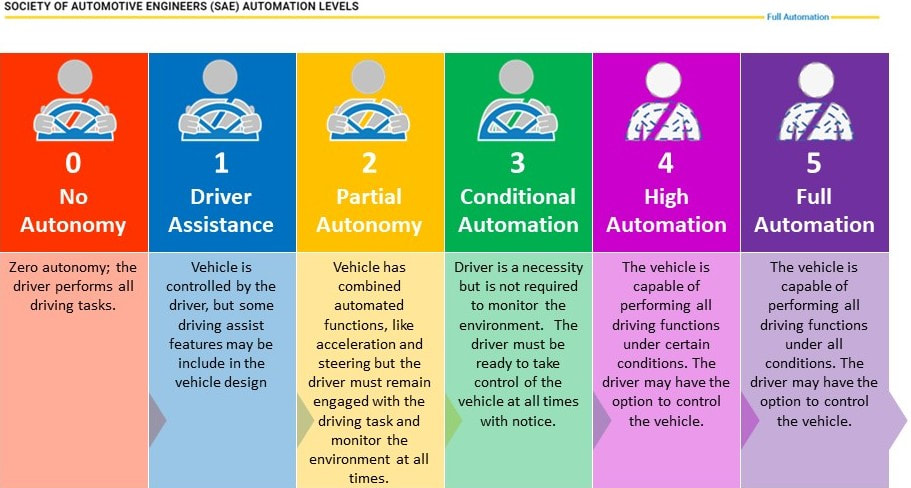
\includegraphics[width=1\textwidth]{levels automation.jpg}
  \captionsetup{justification=centering}
  \captionfont{\small{\textbf{\\Source: \cite{SAE}}}}  
  \label{fig:routerExemplo}
\end{figure}



\subsection{Hardware Architecture}

\begin{figure}[ht]
  \centering
  
  % Caption setup for this specific figure
  \captionsetup{
     labelfont={bf,large},       % label (e.g., "Figure 1:") in bold and large
     textfont={bf,large},        % caption text in bold and large
     justification=raggedright,  % left-align the caption
     singlelinecheck=off         % force left alignment even for short captions
  }
  
  \caption{\MakeUppercase{ADV generic hardware architecture}}
  \label{fig:hardware}
  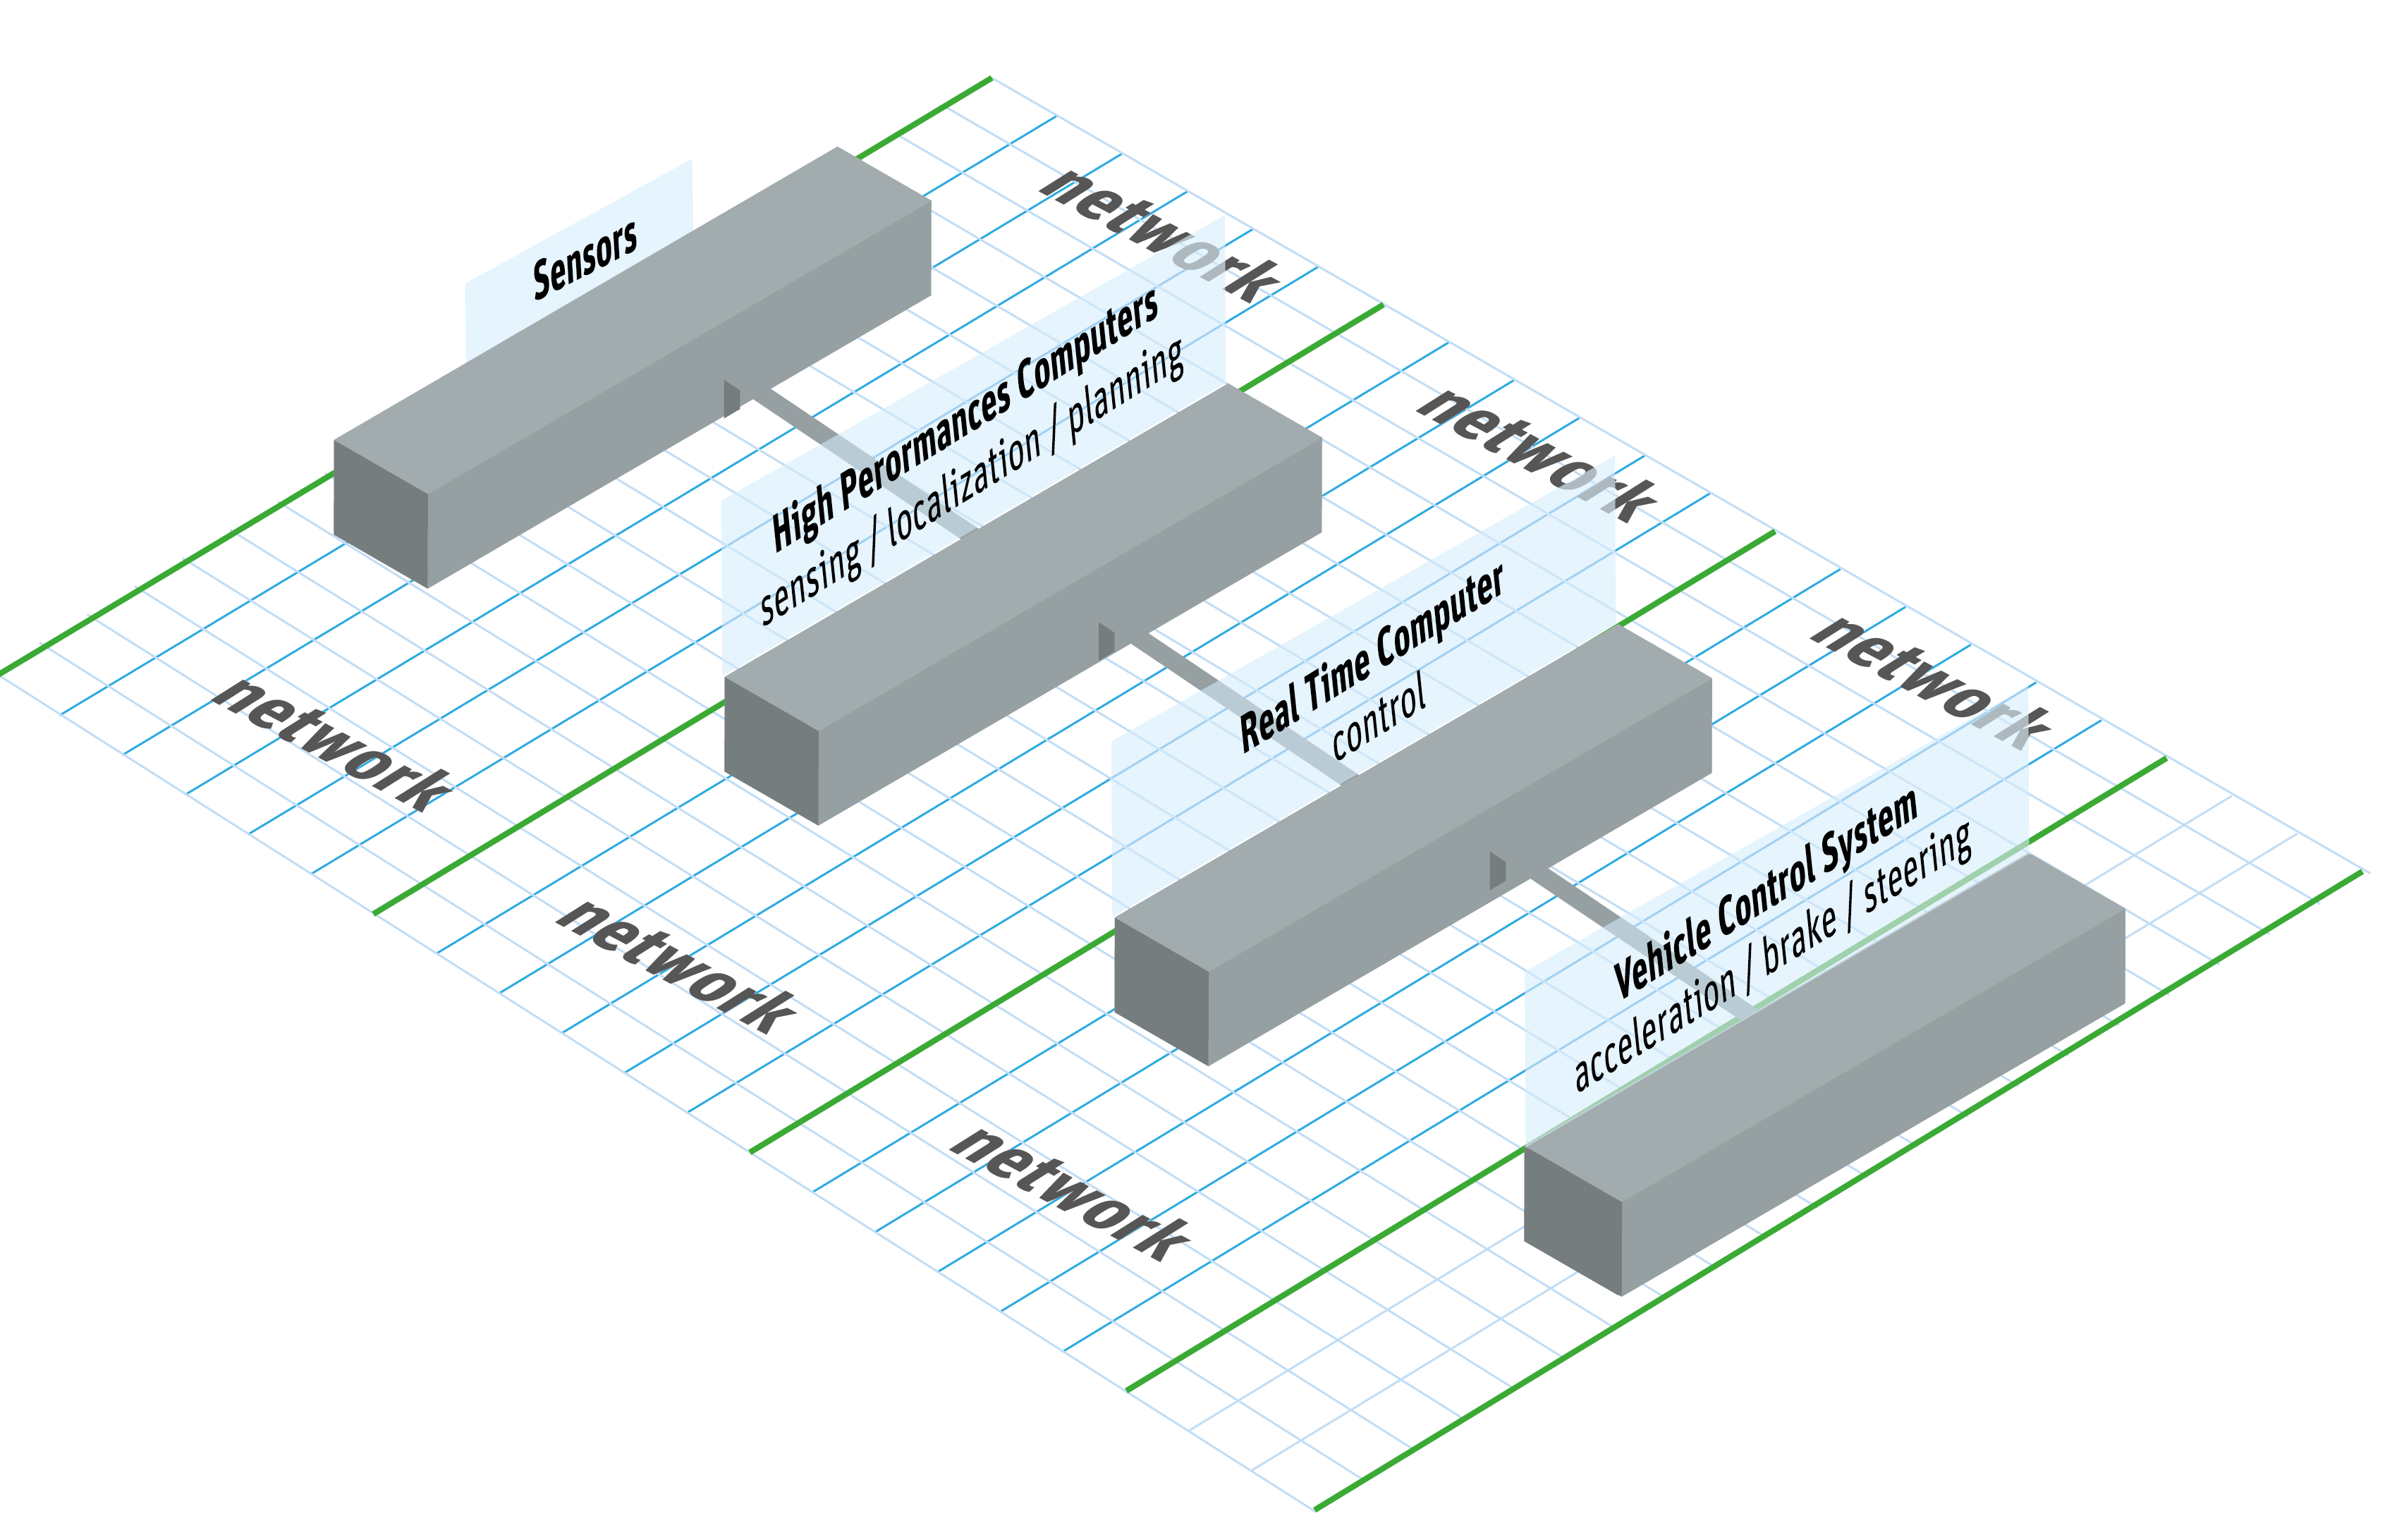
\includegraphics[width=\textwidth, keepaspectratio]{Prancheta 5 (2).png} 
   \captionfont{\small{\textbf{\\Source: \cite{Silva2023}}}}  
\end{figure}

 Figure \ref{fig:hardware} shows the modern hardware architecture of an autonomous vehicle. Sensors are connected through a network to one or more computers. Ethernet and CAN are the most used network protocols for connecting sensors. Usually, the CAN network has the sensors that are provided by the vehicle manufacturer by default, while the Ethernet network is used to insert the new sensors in it \cite{Kessler2019}. In addition, the usb protocol can also be used to connect cameras \cite{Munir2018} or Lidar \cite{Broggi2015} to the computing system.

The ADV computing system could be divided into two parts. The high-performance computers are the components of the architecture where the most computational intense tasks are performed which are sensing, localization, and planning. It involves challenges like point cloud and convolutional neural network (CNN) processing within the time window required for safe and correct actions of the ADV prototype. The real time computer is responsible for the control functions of the vehicle: acceleration, brake and steering. As the name says, it performs real time actions that are critical for the correct response for the commands sent by the high-performance computers. 

The connection between the high processing computer and the real time computer is implemented using Gigabit Ethernet while the connection between the real time computer and the vehicle control system is done using the CAN network.\cite{tang2018}

With the consolidated hardware architecture the choice of high performance computers falls onto high end computers available at the market. The family of Intel I7 processor was found in quite a few ADV prototypes \cite{Kessler2019}
\cite{Betz2019}
\cite{Marin-Plaza2019}
\cite{Reke2020}.
This also brought the development of computers specific designed to autonomous application. There are two leading companies in this development. For the real time computer, the Nvidia Drive Series \cite{NvidiaDrive} provides hardware and software to support the ADV development. For the control system, the Dspace Micro Autobox \cite{dSpace} is a computer with a real time processing system that provides the necessary time constraints for the correct vehicle control. 

\subsection{Software Architecture}


\begin{figure}[ht]
  \centering
  
  % Caption setup for this specific figure
  \captionsetup{
     labelfont={bf,large},       % label (e.g., "Figure 1:") in bold and large
     textfont={bf,large},        % caption text in bold and large
     justification=raggedright,  % left-align the caption
     singlelinecheck=off         % force left alignment even for short captions
  }
  
  \caption{\MakeUppercase{ADV generic software architecture}}
  \label{fig:software}
  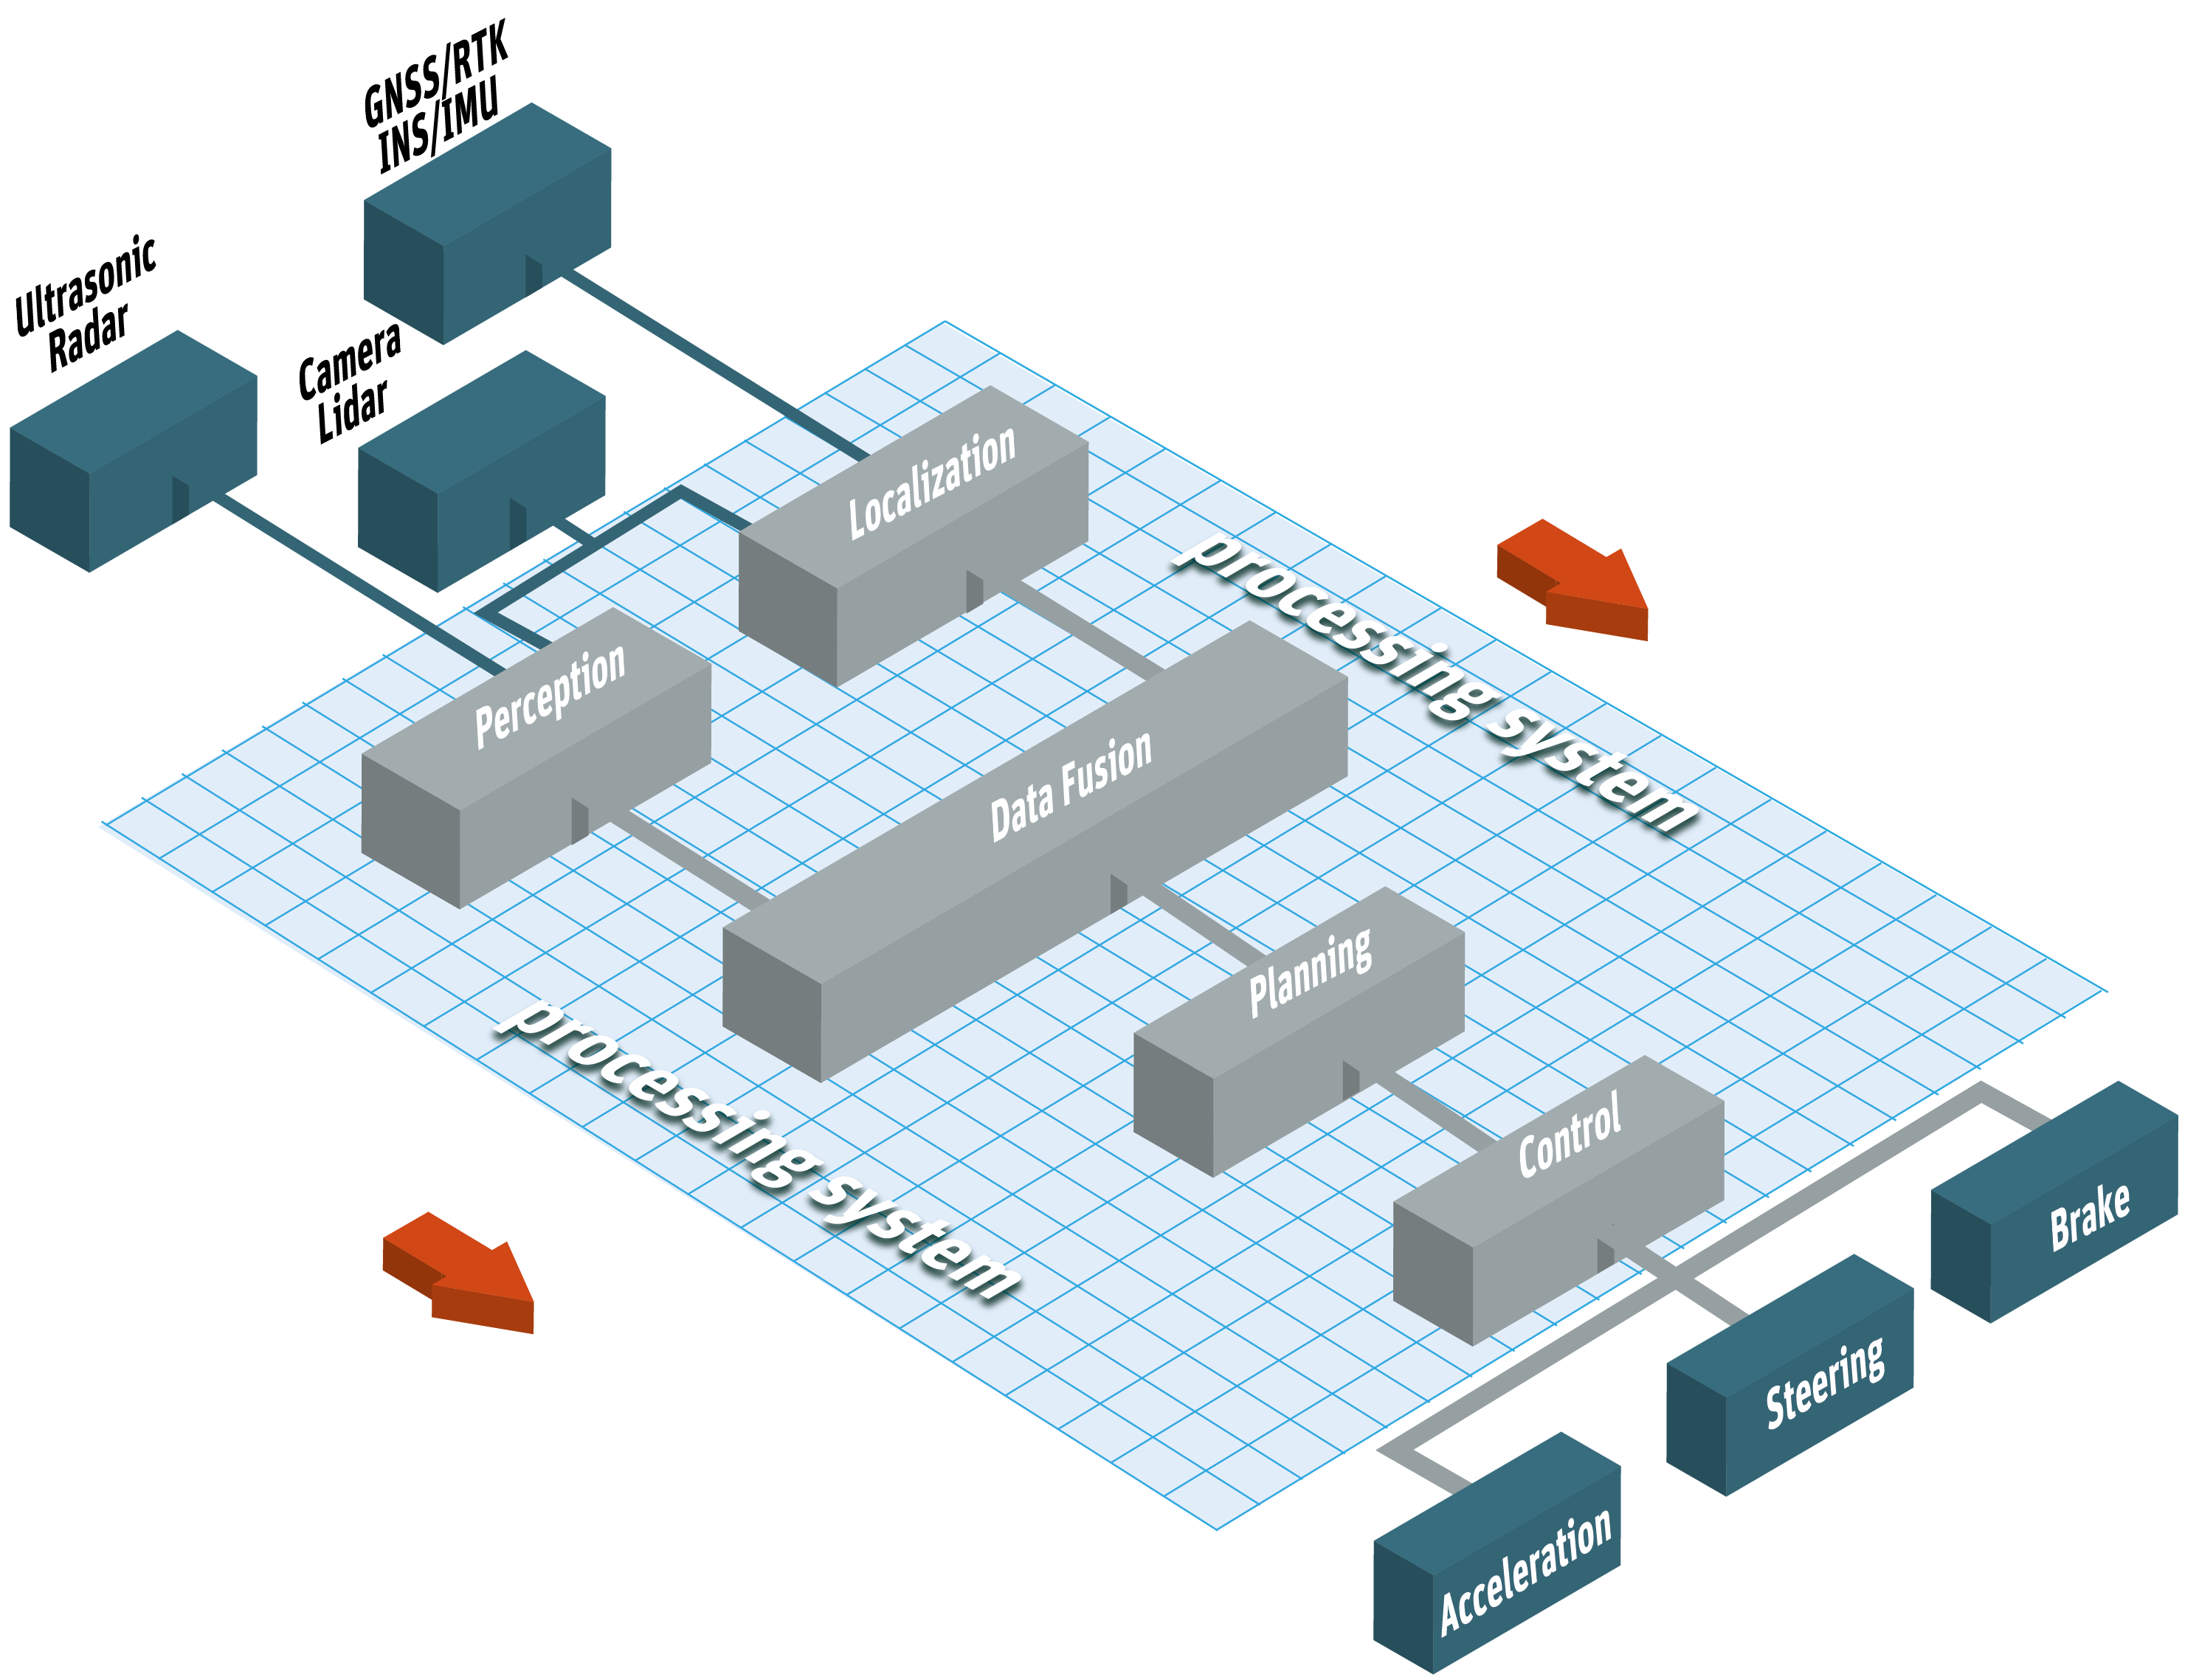
\includegraphics[width=\textwidth, keepaspectratio]{Prancheta 1 (1).png} 
  \captionfont{\small{\textbf{\\Source: \cite{Silva2023}}}}
\end{figure}

 The generic software architecture for ADV is represented in Figure \ref{fig:software}. That is an architecture for an autonomous vehicle with all the functionalities expected of it so it can be deployed in the real world. \cite{Zhou2019}. The processing system, as mentioned above, is made up of one or more computers. Although there are various computer configurations, the operational system and middleware are practically an unanimous choice among researchers being based on Linux distributions and Robot Operating Systems(ROS). %These will be covered with more details later in this Thesis along with other approaches
 
 In addition, the are libraries developed specific for machine learning applications applied in ADV development. In particular OpenCV and TensorFlow. OpenCV is an open source computer vision library that can handle images and videos \cite{jain2018} and is most used in ADV for image collection and processing. TensorFlow is a library that allows one to build and train a deep learning model \cite{chaitra2020} and is mostly used to classify images captured by the ADV. The OpenCV is progressing in its machine learning functionalities, but developers prefer to build the deep learning model on TensorFlow and import it to be applied by the OpenCV. TensorFlow, that is designed by Google, has gain such a momentum that Tensor Processors Unit (TPU) started to be developed specific to accelerate TensorFlow library operations. \cite{TensorFlow}


\subsection{Sensor Set}

There are six main sensors necessary to build an autonomous vehicle. These are required to sense the vehicle surroundings and send information to the computing system. Following each sensor will be explained.

The Lidar (light detection and ranging) is an important sensor that can be used for perception and localization. It produces point cloud data that can be processed to map the environment and locate the ADV and to detect objects and measure their distance \cite{Kato2015}.  It can be processed in popular libraries such as OpenCV. That sensor is the barrier to popularizing the ADV due to its high cost, which can reach \$75,000 dollars \cite{Lin2018}.

The camera is also applied to localization and perception. Various types of cameras applied to ADV were found that ranged from static and moving cameras, monochrome and color cameras, stereo cameras, spherical cameras, and smart cameras. The ones applied to autonomous vehicles are very powerful cameras that could get up to 4416 x 1242 \cite{Karaman2017}, which is higher than the full Hd resolution commonly seen in television transmissions.

The radar is used for obstacle detection in the area surrounding the vehicle in short, medium and long range as part of the perception system \cite{Tas2018a}. It provides precise range and velocity measurements compared to cameras at the cost of less accurate classification capabilities \cite{Kunz2015}. Thus, it is often used together with other sensors such as a Lidar, cameras and GNSS system.

Ultrasonic is an ultra-low range sensor, up to 5 meters detection range, that supports the vision system in low speed tasks such as parking \cite{Zong2018}. Today, these ultrasonic sensors are manufactured in vehicles and its information can be acquired through vehicle CAN buses.

The Global Navigation Satellite System (GNSS), composed of regional systems around the world (GPS, Galileo, Glonass, Compass), provides global ADV localization at an update frequency of 10Hz and a precision of 6 meters, which is not enough for real-time applications \cite{Liu2019}.  GNSS precision can be improved by using the real-time kinematic (RTK) system that corrects the GNSS information and reduces precision to centimeters \cite{Buyval2019}. 

To improve the update rate of the GNSS systems, the inertial navigation system (INS) is also combined with the GNSS signals. The INS uses the signal provided by another sensor, called an inertial measurement unit (IMU). However, its accuracy degrades over time, which does not allow its use alone. Therefore, the combination of RTK, GNSS, and INS systems would provide an accurate vehicle location in real time \cite{Liu2019}.

\subsection{Simulators}
Testing and development have increasingly relied on simulation environments to address the limitations and risks associated with real-world road tests. Traditional road tests require significant time and resources and involve high costs and potential safety risks, particularly when testing extreme driving conditions or edge cases. To overcome these challenges, a variety of simulators have been developed to provide a cost-effective, safe, and efficient way to validate ADV performance in diverse scenarios \cite{Zhang2024}.

Simulation environments allow for efficient testing of ADVs under controlled and repeatable conditions. These environments can replicate diverse scenarios, such as various weather conditions, unexpected obstacles, or complex traffic conditions, which would be impractical or unsafe to recreate in the real world. They also enable the collection of substantial volumes of training data, which is crucial for machine learning models used in autonomous systems. \cite{Zhou2022}. Furthermore, simulators provide advantages for academic researchers and developers with limited access to a physical testing infrastructure. Open-source simulators, in particular, have lowered the barrier to entry for those without access to expensive hardware, fueling collaboration and innovation within the research community \cite{Li2024}.

Although simulators provide immense benefits for testing ADV systems, they are not without limitations. Issues such as sensor emulation fidelity, vehicle dynamics precision, and realistic representation of traffic participants can affect the transferability of simulator-trained models to real-world applications \cite{Li2024}. In addition, the construction of virtual maps and environments remains labor intensive, limiting the scalability of simulations.

The research community recognizes three types of simulations \cite{Rosique2019}: live, virtual, and constructive simulations. Each type differs according to the level of realism and the interaction with actual hardware components.

\begin{itemize}
\item \textbf{Live Simulations}: Live simulation is an operational test involving real components, such as vehicles and sensors, used in an environment that closely resembles real-world conditions. It is the closest type of simulation to real use, involving actual forces and equipment to assess which systems have been damaged or how they respond under realistic conditions.
\item \textbf{Virtual Simulations}: These simulations, also referred to as \textit{X-in-the-loop}, involve testing a complete system or its components using a stimulus generated by a computer or through other artificial means. Virtual simulations are ideal for software-in-the-loop testing, where autonomous driving software can be evaluated in a controlled environment before deploying on physical hardware.
\item \textbf{Constructive Simulations}: Constructive simulations are entirely computer-based and do not involve any physical components. They represent a system or multiple systems virtually and can be used to test how these systems react to different inputs. Constructive simulations are valuable for modeling complex scenarios, such as interactions between multiple components, without the need for expensive physical setups.
\end{itemize}

%\subsubsection{CARLA simulator}

%CARLA (Car Learning to Act) is an open-source simulation platform designed to facilitate the development, testing, and validation of autonomous driving systems \cite{Dosovitskiy2017}. Provides an urban environment where researchers can simulate complex driving conditions, including changes in weather, pedestrian movements, and vehicle behaviors. Built on Unreal Engine 4, CARLA offers high-fidelity 3D environments, making it suitable for academic research and industry applications. %\cite{CARLA}

%CARLA's sensor suite, which includes cameras, LIDAR, radar, and GPS, allows developers to simulate a wide range of real-world conditions. This supports the testing of perception, localization, and control algorithms. Moreover, CARLA offers flexible API support, enabling integration with Python and C++ for logical interaction with autonomous driving stacks. The platform is also highly customizable, allowing users to modify the environment, sensor settings, and traffic scenarios, creating a rich testing ground for autonomous systems.




\subsection{Datasets}

The development of autonomous driving vehicles (ADV) is fundamentally based on robust perception and decision systems capable of understanding highly dynamic and complex environments \cite{feng2020}. The effectiveness of these systems is directly proportional to the amount and quality of data used for their training and validation. Without extensive and high-quality datasets, the ability of ADVs to generalize across diverse scenarios remains severely limited.

An autonomous driving vehicle (ADV) dataset is a structured collection of sensor data recorded from real or simulated driving environments, used to train, validate, and benchmark perception and decision-making algorithms. These datasets typically include multimodal sensor inputs, such as RGB or grayscale camera images, LiDAR point clouds, radar signals, and GPS/IMU measurements for accurate localization.

In addition to raw sensor data, they often contain ground-truth annotations, including object detection labels such as bounding boxes and 3D bounding volumes, semantic segmentation maps, lane markings, and tracking information across frames. Some datasets also provide map data, traffic signal states, and environmental metadata such as weather and time of day.

It is estimated that achieving a safety level comparable to human drivers would require driving billions of kilometers under varied conditions, a task that is practically impossible only through real-world tests \cite{angeletti2023}. This constraint has led to the widespread adoption of publicly available datasets and simulation-based synthetic data generation to accelerate development while maintaining safety and cost efficiency.

%Recognizing the need for scale and diversity, Waymo Open Dataset (WOD) was introduced. WOD provides over 1150 scenes, each spanning 20 seconds, collected across different cities such as San Francisco, Phoenix, and Mountain View. It offers more than 12 million 3D LiDAR bounding box annotations and 9.9 million camera labels \cite{sun2020}.

%The WOMD-LiDAR dataset expands motion forecasting research by providing raw LiDAR data for more than 100,000 scenes, addressing limitations of previous datasets that only offered abstracted representations like bounding boxes \cite{chen2024}.  An extensive number of other open datasets in the real world prior to 2019 can be found in the survey by \cite{kang2019} and a more up-to-date review of available datasets can be found in \cite{liu2021} and \cite{liu2024}.

Real-world data collection can be expensive, time-consuming and challenging to scale \cite{feng2020}. Furthermore, real-world datasets often suffer from a long-tail distribution of scenarios, where rare but critical events such as accidents and unusual weather conditions are rarely presented \cite{song2024}. Gathering more data and corner cases is becoming more critical than inventing new deep neural network architectures. Collecting such data in the real world can be dangerous or infeasible. 

Therefore, synthetic datasets generated from 3D game engines, offer a cost-effective and scalable alternative, allowing researchers to create customized scenarios and accelerate their research results. However, this introduces a new set of challenges: ensuring that synthetic data accurately reflect the complexities of the real world, including sensor noise, object textures, and physical dynamics.


\subsection{WorkLoad}
Autonomous vehicles are relying on complex computer systems to perceive their surroundings, plan their actions, and control the vehicle. The computational demands of these systems, often referred to as workload, are a critical factor in ensuring the safe and efficient operation of ADVs. Understanding and characterizing this workload is essential to optimize resource allocation, manage power consumption, and guarantee real-time performance. Accurately estimating the performance of perception systems requires models that consider available resources. 

These workloads are typically heterogeneous, involving a mix of tasks such as data acquisition, image preprocessing, neural network inference, and multisensor fusion, all of which must operate under strict real-time constraints. The performance of such systems is not solely dependent on algorithmic accuracy, but also on the ability to process data efficiently across different hardware architectures, including CPUs, GPUs, and specialized accelerators \cite{Tang2022CharacterizationEdge}.

The dynamic nature of driving environments introduces significant variability in workload. Factors such as traffic density, weather conditions, and the complexity of the surrounding environment can all impact the computational demands of ADV systems. 

For example, driving in heavy traffic or adverse weather conditions requires more intensive processing of sensor data to accurately detect and track other vehicles and obstacles. Such variabilities may also contribute to burst computation and memory access, potentially leading to increased tail latency and impacting safety \cite{Liu2023COLA:Systems}

Characterizing the workload involves understanding the types of data being processed and the nature of the algorithms being used. As ADV applications are mainly focused on detection, recognition, and prediction, workloads often fall into the domains of computer vision, machine learning, and deep learning \cite{wang2018}.

Therefore, one of the main challenges in this domain lies in defining consistent performance indicators to compare algorithms in varying datasets and hardware setups \cite{Kowalczyk2022EfficientVerification}. Furthermore, recent studies highlight that preprocessing stages, such as image decoding, resizing, and sensor calibration, are often overlooked, despite contributing significantly to overall latency \cite{Bachkaniwala2024Lotus:Profiling}.

Effective workload management is essential to maintain the performance and safety of autonomous vehicles. This involves techniques such as dynamic task scheduling, resource allocation, and adaptive algorithm selection. By carefully characterizing and managing the workload, it is possible to optimize the performance of ADV systems, ensure timely responses to critical events, and ultimately achieve higher levels of driving automation.

%%%%%%%%
%\section{Operational Systems and Framework} \label{memorias}

%Most of the developed solutions to deal with the complexity of managing all the hardware involved in the ADV range from using operating systems or frameworks. However, it has been seen that there was not a preferred choice or consolidation on that and the manufacturers and researches keep developing new frameworks and operating systems for autonomous applications.

%An Operating System (OS) is a set of programs that controls the interactions between the complex system hardware and the user applications. It acts as a translator between the hardware and the user \cite{holcombe2020}. An OS to act as a computer interface creating an abstraction from the machine language used to control a computers hardware and to manage resources available in a machine like memory and processor execution time \cite{stallings2018} 


%MIddleware is a software technology that abstracts the low level details of a system from the user application. It allows modular connection of distributed software \cite{astley2001}. It can be used in distributed heterogeneous systems putting together different pieces of software, from different applications, and delivering it to the variety of hardware available on the system. It simplifies software development especially in systems with many services and tight interaction between them \cite{Liu2019}.

%The big difference between them is that middleware run on top of an operating system relying on it to access machine resources. It is a preferred choice to avoid the burden of developing a OS from scratch but bring extra software layers that could bring down the whole system efficiency.


%\subsection{Real Time Operating Systems}
%A real time response within time constraints is a key aspect of an autonomous vehicle system. For this purpose a real time operating system (RTOS) is one of the choices to manage the vehicle hardware system. The RTOS is characterized as having time as a key parameter. That means that it is deterministic as it performs operations within a predefined time interval \cite{stankovic2004}.

%Generic operating systems have the processes competing for processor time and resources within the CPU. In a RTOS the execution of determined process is determined by external interruptions or fixed time intervals. For a deterministic system the processing time and system resources must be enough so that it can respond to any request in the determined period of time \cite{stallings2018}

%In addition, the real-time systems are divided into hard and soft. The soft real-time systems are the ones that a missing deadline would not cause any permanent damage to the system. On the other hand, in the hard real-time system any missing dead line would cause permanent damage to the system. RTOS are also applied into embedded operating systems that are designed to control a specific device like vehicles, phones or TVs \cite{tanenbaum2015}.


%\subsection{Autonomous Vehicles Framework}
%The rise of autonomous vehicles technology make it clear the necessity to deal with the specific aspects of its hardware. Called supercomputers on wheels, ADV software has been evolving from embedded software running on a RTOS to a complete middleware with many software components, libraries and modules \cite{velasco2020}. Many sensors and complex logic and algorithm needed to be processed. Some already known in the robotic electronics field and some only applied in the ADV itself. Avoiding making a new SO from scratch, developers opted to make a middleware to run on the top of an operating system to deal with the ADV system hardware and algorithms.

%Autonomous vehicles middlewares tend to be modular and to follow patterns in the future due to the development of the artificial intelligence applied on it and the autonomous vehicles architecture consolidation \cite{Li2018}. The next years will serve the purpose to test the vehicles middlewares and to make clear all its necessary functionalities Nowadays, the middleware modules are perception, planning, localization, data fusion and control.
\section{Heterogeneous Computing Systems}
Heterogeneous computing involves the use of multiple types of processor, each optimized for different tasks, within the same system. The primary goal of this architecture is to achieve high performance while maintaining power efficiency. In heterogeneous systems, CPUs are often combined with other specialized processing units, such as GPUs or FPGAs, to take advantage of the strengths of each type of hardware. \cite{Zahran2019}.

From a hardware perspective, heterogeneous systems may include differences in memory systems, interconnection networks, and processor capabilities. The use of different memory technologies, such as DRAM and non-volatile memory, as well as differences in cache hierarchy and access times, contribute to the complexity and heterogeneity of such systems. This variety in hardware components allows flexibility in optimizing specific tasks for performance or energy efficiency, but also introduces challenges in programming and workload distribution \cite{Zahran2019}.

GPUs have become widely used as coprocessors in many embedded systems to speed up general-purpose applications. Their multithreaded architecture and high-bandwidth memory make them especially suitable for data-parallel tasks. Using GPUs, many embedded systems can achieve both high performance and improved energy efficiency. For instance, GPUs can effectively handle operations such as matrix factorization, multidimensional FFTs, and convolutions, which are frequently required in signal processing, imaging, and video applications. \cite{li2021}

The integration of CPUs and GPUs is particularly popular due to the complementary nature of these processors; CPUs perform better at serial task execution, while GPUs are ideal for parallel workloads, such as machine learning and computer vision \cite{Han2021}. By applying new programming models, such as CUDA and OpenCL, developers can effectively create highly data-parallel tasks that take full advantage of GPU capabilities. In the context of autonomous vehicles, GPUs can be used to accelerate tasks such as training and inference of neural networks, which are essential to processing visual and sensor data in real-time environments \cite{Hazarika2020}.

\subsection{Programming libraries for Heterogeneous Computing Systems}

Programming libraries for heterogeneous systems can be categorized into explicit and directive-based models. Directive-based models, such as OpenMP and OpenACC, use annotations to guide compilers in task allocation, making it easier for developers to utilize multiple processing units without extensive code rewriting. The compiler handles the details of mapping code to different processors, allowing greater flexibility. Explicit models, such as OpenCL and CUDA, require developers to manually manage the task distribution between processors, offering more control but requiring deeper hardware understanding \cite{Terzo2019}.

These programming libraries aim to simplify the distribution and allocation of workloads, allowing developers to focus on application development rather than hardware management \cite{Brandejsky2022}. In addition, it provides a homogeneous view of the computing environment, while also allowing the developer to make low-level optimizations as necessary. Ensuring portability is critical in heterogeneous computing, as applications need to run efficiently across a range of hardware configurations. Strategies for achieving portability include high-level abstractions, low-level details, runtime management, and on-the-fly code modification using techniques such as continuous compilation or binary optimization \cite{Zahran2019}.

Managing communication overhead between the CPU and accelerators is a key challenge. Techniques like streaming help reduce this overhead by overlapping data transfer with computation, improving system throughput \cite{Fang2020}. There are several programming models. In the following, we will concisely describe the most popular ones.

\begin{itemize}
    \item \textbf{CUDA (Compute Unified Device Architecture)}:  is a programming platform developed by NVIDIA to allow developers to utilize the GPU's processing power for general-purpose computing. CUDA helps developers specify which parts of the code are executed on the GPU, providing detailed control over memory management and task execution on NVIDIA GPUs. This model is particularly useful for accelerating workloads that require intensive computation, such as scientific simulations, deep learning, and image processing.
    \item \textbf{OpenCL (Open Computing Language)}: serves as an open standard for programming on various types of processor, including CPUs, GPUs, and FPGAs. OpenCL enables developers to write portable code that can run on different types of processing unit, making it a versatile option for heterogeneous computing. The explicit management of different devices in OpenCL allows developers to fine-tune their programs for performance across different hardware platforms.

    \item \textbf {OpenMP 4.0 }: is an extension of the OpenMP standard that includes features to target devices such as GPUs and multi-core CPUs. It allows developers to explicitly specify how data and computation should be handled between the host and accelerators. OpenMP 4.0 provides a comprehensive set of directives, such as target, teams, and distribute, to manage the offloading of tasks to GPUs, giving developers greater control over how computations are distributed and executed on different devices.

    \item \textbf {OpenACC (Open Accelerators)}:  was introduced as a standard for simplifying programming on heterogeneous architectures, including multi-core CPUs and GPUs, using a directive-based approach. OpenACC allows developers to annotate their code with pragmas, such as \#pragma acc kernels, to specify which sections should be offloaded to an accelerator. This helps automate the handling of parallel regions, data transfers, and synchronization, making it a user-friendly option for parallelizing applications without major code restructuring.

    
    \item \textbf{SYCL}: Built on top of OpenCL, SYCL provides a higher-level, C++ like interface for single-source programming. Developers can write code for both the host (e.g., CPU) and devices (e.g., GPUs) within the same source file. SYCL simplifies the integration of different processing units while maintaining portability and offering performance optimization options.
    
    \item \textbf{HIP (Heterogeneous-Compute Interface for Portability)}: Developed by AMD, HIP facilitates portability between CUDA applications and AMD hardware. It provides an interface that is largely compatible with CUDA, allowing developers to write code that runs on both AMD and NVIDIA GPUs. This cross-platform flexibility is crucial for applications that need to operate efficiently across different GPU vendors.

    \item \textbf {TensorFlow}: is an open-source platform for machine learning, designed to operate across heterogeneous computing environments. By supporting computations on various hardware such as CPUs, GPUs, FPGAs, TPUs, edge devices, microcontrollers, it enables developers to deploy models in diverse settings, optimizing scalability and performance. TensorFlow's robust deployment capabilities, exemplified by TensorFlow Serving, allow models to run at production scale on advanced processors like TPUs. By internally handling the complexities of task allocation and resource management, TensorFlow abstracts the intricacies of heterogeneous hardware, ensuring efficient utilization of multiple processing units for both training and inference, and allowing developers to focus on model development without concerning themselves with hardware specifics.

%\item \textbf {StarPU} (Ficar no final com um pouco mais de texto) is a task programming library that facilitates programming for heterogeneous systems by defining tasks and managing dependencies, which are then automatically scheduled across available processing units like CPUs, GPUs, and other accelerators. This dynamic scheduling supports optimal resource utilization and efficient load balancing. Unlike directive-based models, StarPU offers explicit control over task definitions while managing resource complexity at runtime.
    
\end{itemize}

\section{Task Scheduling}
\label{sec:task-scheduling}
A Task is a combination of sub-tasks or threads that execute a specific computing objective such as reading sensor data or processing a steering action. Choosing the more efficient task processing sequence based on the necessary resources required from each task is a challenging job for developers. The complexity level gets even higher when dealing with a heterogeneous multiprocessor embedded system such as the ADV. In this case, it is necessary not only to organize a task queue but also to decide which processing unity would be best suitable for each task. In ADV some tasks have better performance using a specific type of processing unity \cite{Liu2017}. 

The scheduler is responsible for scheduling and assigning tasks to processors. It implements an scheduling algorithm that provides a schedule for the system task set that must be feasible and schedulable. This translates into meeting all the time constraints of the system and producing a valid schedule for a set of system tasks. In a real time system the scheduling algorithm must be optimal meaning having both characteristics described above.

In addition, there are static schedulers that are inflexible on handling changes in workloads with fixed rules, and dynamic schedulers that can identify tasks workload changes to take online decisions on the best schedule for that moment. There is no best choice, and the applied system must be evaluated to make the best decision on which way to go. Real time embedded systems could be either predictable or not, which has a direct interference in the scheduling strategy to be chosen. \cite{yang2020}


For autonomous vehicles, some level of efficiency must be achieved in organizing the autonomous vehicle processing tasks. The task miss ratio must be kept to a minimum level to avoid accidents due to non processed data. The total execution time and utilization of hardware resources must be kept at a minimum to reduce energy consumption and keep vehicle autonomy at maximum levels.

\subsection{Basic Concepts}
A process or task \cite{chakraborty2024} generally goes through phases of CPU bursts (computation) and I/O bursts (waiting for input/output operations). Task scheduling is about optimizing the use of the CPU during these bursts to ensure that no CPU resources are wasted while a task waits for I/O operations to complete. Interactive tasks tend to have shorter CPU bursts and more frequent I/O, such as a word processor waiting for user input, while compute-intensive tasks have longer CPU bursts, spending more time executing computations, like a video transcoder.

The goal of task scheduling is to maximize CPU utilization (keeping the CPU as busy as possible, ideally between 40\% for lightly loaded systems to 90\% for heavily loaded systems) and throughput (the number of processes completed per unit time) while minimizing waiting time (time spent waiting in the ready queue), response time (time from submission until the first response) and turnaround time (total time from submission to completion of a process)\cite{silberschatz2018}. Different CPU scheduling algorithms have distinct properties, and the choice of algorithm may favor certain types of processes. It is also important to consider the variance in response time, especially for interactive systems, where predictable response times are often preferred to minimizing average response times.

There are two types of scheduling methods: preemptive and non-preemptive scheduling. In non-preemptive scheduling, a running task retains control of the CPU until it either terminates or moves to a waiting state. In preemptive scheduling, the operating system can forcefully remove a task from the CPU when a higher priority task needs to be executed or when a time slice dedicated to that task expires, which is crucial for maintaining good response times for interactive tasks \cite{krzyzanowski2015}.

To achieve effective scheduling, a scheduler manages tasks that are ready to execute and decides the next task to allocate to the CPU. The ready queue stores tasks waiting to be executed, while waiting queues manage tasks blocked by I/O operations. The scheduling algorithm used determines the performance characteristics of a system, with goals such as fairness, efficiency, and minimal overhead \cite{silberschatz2018}.

Schedulers can be classified into different types: long-term, medium-term, and short-term schedulers. The long-term scheduler decides which tasks should be brought into the ready queue, ensuring a good mix of I/O-bound and CPU-bound tasks to achieve optimal CPU utilization. The short-term scheduler selects from the ready queue which tasks should be executed next, making rapid decisions to keep the CPU busy. The medium-term scheduler is responsible for managing tasks that are swapped out of memory to reduce the degree of multi-programming, often used to optimize memory utilization \cite{chakraborty2024}.

\subsection{Traditional Scheduling Algorithms}

Scheduling algorithms are central to how operating systems manage CPU resources among multiple tasks. Over the years, various scheduling algorithms have been developed, each with unique characteristics that make them well suited for particular scenarios and types of workload. These algorithms aim to optimize resource utilization, minimize waiting time, and ensure fairness across tasks. Schedulers often have to balance between being fair, ensuring every process has an opportunity to execute, and efficient, keeping the CPU as busy as possible. Below follow some of the traditional scheduling algorithms.

\textbf{First-Come, First-Served (FCFS)} is the simplest type of CPU scheduling algorithm. In FCFS, processes are executed in the order in which they arrive in the ready queue. This non-preemptive algorithm ensures that the task that requests the CPU first gets it first. However, FCFS can cause the convoy effect, where shorter tasks have to wait for a long-running task to complete, resulting in an increased average waiting time and poor CPU utilization, especially in systems with mixed workloads \cite{silberschatz2018, tanenbaum2015}.

\textbf{Round Robin (RR)} scheduling is a preemptive algorithm that assigns a fixed time quantum to each task in the ready queue. Each task is executed for the duration of the time slice, after which it is preempted and placed at the back of the queue if it is not yet complete. RR is particularly effective for time-sharing and interactive systems, as it ensures that all tasks receive equal CPU time, thus improving responsiveness. However, the choice of the time quantum is critical, as a small quantum can lead to a high context-switching overhead, while a large quantum reduces the benefits of preemption \cite{silberschatz2018,padallan2023}.

\textbf{Shortest Job First (SJF)} scheduling selects the task with the shortest next CPU burst. SJF can be either preemptive or non-preemptive and is considered optimal for minimizing average waiting time. However, SJF requires knowledge of the duration of future CPU bursts, which is difficult to estimate in practice. Despite this limitation, it is effective in environments where the nature of tasks is predictable. One drawback of SJF is the potential for starvation, where longer tasks may never be scheduled if shorter tasks keep coming. \cite{tanenbaum2015, padallan2023}.

\textbf{Priority Scheduling} assigns priorities to tasks and allocates CPU to the tasks with the highest priority. This algorithm can be preemptive or non-preemptive, depending on whether a higher priority task can preempt the current task. It is often used in systems that need to distinguish between more important and less important tasks. One of the key challenges of this algorithm is starvation, where low priority tasks may be indefinitely delayed. To mitigate this, aging can be applied to gradually increase the priority of waiting tasks \cite{chakraborty2024, tanenbaum2015}.

\textbf{Multilevel Queue Scheduling} divides tasks into different queues based on characteristics such as priority or type. Each queue may use a different scheduling algorithm and have a specific priority level. For example, interactive tasks might be assigned to a high priority queue using Round Robin, while batch tasks are handled in a lower priority queue with FCFS. This approach provides flexibility in effectively managing different types of workload, ensuring that high priority tasks receive more immediate CPU attention \cite{silberschatz2018,tanenbaum2015}.


\subsection{Real-Time Task Scheduling}

Real-time task scheduling is critical in systems where tasks must meet strict timing requirements. Real-time systems are computing environments where the correctness of operations depends not only on logical results but also on the time at which these results are produced. These systems must respond to input or events within strict deadlines, ensuring deterministic behavior \cite{Burns2009}.

These systems are classified into hard real-time systems and soft real-time systems. Hard real-time systems require absolute adherence to deadlines; missing a deadline is considered a critical failure. Examples include flight control systems and medical life support systems. In contrast, soft real-time systems are those where meeting deadlines is important but occasional deadline misses are tolerable,although losing some system performance. Multimedia streaming applications and online transaction systems are typical examples of soft real-time systems. \cite{Buttazzo2020}

According to \cite{tanenbaum2015} and \cite{pandit2013}, the main characteristics of real-time systems are determinism, reliability, responsiveness, concurrency, and fault tolerance. Determinism refers to predictable system behavior, with responses occurring within defined time bounds. Reliability is another characteristic, and often real-time systems have mechanisms to mitigate and minimize the impact of failures in their operation. Responsiveness is crucial, requiring the system to respond quickly to external events or incoming data, especially in embedded control systems where timing is critical. Managing multiple tasks simultaneously requires effective handling of concurrency, and techniques such as priority inheritance protocols are used to avoid priority inversion issues during concurrent task execution. Fault tolerance is the ability of the system to continue operation, possibly at a reduced level, rather than failing completely when some part of the system fails.


Real-time task scheduling algorithms are developed to ensure that all tasks meet their deadlines, maintaining the system's reliability and predictability. Unlike traditional systems, which prioritize throughput and CPU utilization, real-time systems focus on ensuring that tasks are completed within their deadlines. Applications include embedded systems, industrial automation, robotics, and other scenarios in which failure to meet time requirements can have catastrophic outcomes. The following are the most common algorithms found in the literature \cite{abdullah2023real, pandit2013, davis2011, silberschatz2018, Buttazzo2020}.


\textbf{Rate-Monotonic Scheduling (RMS)} is a static priority scheduling algorithm used for periodic tasks in real-time systems. In RMS, tasks with shorter periods are assigned higher priorities based on the assumption that tasks that require more frequent execution should be prioritized to meet their deadlines. RMS is optimal for fixed-priority scheduling of periodic, independent tasks with known execution times. However, it may become inefficient if the task priorities are not assigned properly or if the system is heavily loaded.


\textbf{Earliest-Deadline-First (EDF)} is a dynamic priority scheduling algorithm in which the task with the closest deadline is given the highest priority. EDF is optimal for maximizing CPU utilization, as it always selects the task closest to its deadline. This algorithm is widely used in real-time systems due to its flexibility in managing tasks with varying deadlines. Unlike RMS, EDF can handle higher CPU utilization and adapt to changes in task deadlines, making it suitable for complex real-time environments.


\textbf{Fixed-Priority Scheduling with Preemption} assigns static priorities to tasks, with the scheduler always selecting the highest priority task for execution. Preemption allows a higher priority task to interrupt a lower priority one, ensuring that critical tasks meet their deadlines. Although preemption introduces overhead due to context switches, it is necessary to guarantee deadlines for high priority tasks. This method is similar to priority scheduling in traditional systems, but is adapted for real-time requirements where timing is crucial.


\textbf{Event-Driven Scheduling} is utilized in systems where tasks are triggered by specific events. Tasks are activated by external or internal stimuli, such as sensor inputs or data availability. This scheduling approach is suitable for systems that must react promptly to external events, ensuring that critical situations are addressed without unnecessary delays. It is ideal for embedded systems and industrial applications where immediate response is essential.

\subsection{Heterogeneous System Task Scheduling}

Task scheduling in heterogeneous computing systems is essential to efficiently utilize diverse processing units, such as CPUs, GPUs, and other specialized accelerators. These systems provide a powerful solution to perform computationally intensive tasks that require different types of processing capabilities. The objective of heterogeneous task scheduling is to allocate tasks to the appropriate processors to minimize the overall execution time (makespan) while ensuring efficient utilization of resources \cite{Fan2016}.  Cloud platforms, such as Amazon AWS and Microsoft Azure, utilize task scheduling algorithms to effectively manage resource allocation and ensure quality of service (QoS) for users \cite{Yiheng2024}.

Heterogeneous computing systems consist of various processors with different capabilities, which introduce challenges such as varying processor speeds, distinct architectural characteristics, and communication overhead. Efficient scheduling of tasks in these systems is key to achieving high performance, especially for complex applications represented by Directed Acyclic Graphs (DAGs), where the nodes represent tasks, and the edges represent dependencies between tasks \cite{Amalarethinam2015}. 

Heuristic scheduling methods are one of the primary approaches for handling task allocation in heterogeneous systems. These methods rely on rule-based heuristics or human experience to make scheduling decisions. Heuristic-based scheduling can be further classified into list scheduling, clustering-based, and task duplication methods\cite{AlEbrahim2017,Fan2016}.

List scheduling involves constructing a task queue sorted by priority, where tasks are sequentially allocated to processors that can execute them at the earliest possible time. This approach is relatively simple to implement and is widely used due to its low time complexity and effectiveness in heterogeneous systems. In clustering-based scheduling, tasks that communicate frequently are grouped into clusters, which are then assigned to the same processor to minimize communication overhead. This approach aims to reduce the inter-processor communication cost, therefore improving the efficiency of task execution in heterogeneous environments. 

Task duplication scheduling aims to duplicate predecessor tasks across different processors to avoid communication delays. This approach is beneficial when the communication cost is high, as duplicating tasks can reduce the overall makespan and improve the system performance.

Dynamic scheduling methods make scheduling decisions at runtime, adapting to changes in the system environment, such as varying processor loads or task arrival times. This approach is suitable for environments where task characteristics and processor availability cannot be determined in advance. Dynamic scheduling methods are particularly useful for heterogeneous systems, where processors may have different performance characteristics and need to adapt based on real-time conditions \cite{Xie2019}. 

The metrics used to evaluate effectiveness of scheduling methods in heterogeneous systems are minimizing makespan, used to evaluate scheduling in all types of system, and the specific metrics for heterogeneous multiprocessing systems that are load balancing across all available processors and energy efficiency, especially in large-scale systems.

Scheduling in heterogeneous systems faces several challenges. The presence of diverse processing units with different architectures and computational capabilities makes task scheduling complex. Allocating the right task to the appropriate processing unit requires careful consideration of the processors characteristics and the tasks requirements \cite{AlEbrahim2017}. Additionally, the communication cost between different processing units can significantly impact performance, particularly in tasks with high interdependency. Minimizing this overhead is essential to achieve efficiency in heterogeneous systems \cite{Amalarethinam2015}.

Based on a review of various references \cite{Amalarethinam2015,Xie2019, Alam2018, AlEbrahim2017, chen2017, singh2016}, the following scheduling algorithms and heuristics are among the most commonly used in heterogeneous computing systems:

\textbf{Heterogeneous Earliest Finish Time (HEFT)}  assigns tasks to processors by evaluating their execution costs, and prioritizes tasks based on a rank that accounts for both computation and communication costs. HEFT is known for achieving good trade-offs between makespan and resource utilization, making it suitable for diverse application scenarios.

\textbf{Critical Path on a Processor (CPOP)} is an extension of the critical path method specifically designed for heterogeneous systems. It selects the processor that minimizes the total completion time of tasks along the critical path. This algorithm is effective in optimizing task allocation, particularly for applications where task dependencies play a significant role in performance.

\textbf{Min-Min and Max-Min} are heuristic scheduling strategies that are often used in heterogeneous systems. The Min-Min strategy selects the task that can be completed the earliest and assigns it to the processor that minimizes its completion time. Max-Min, on the other hand, assigns the longest task first to avoid situations where large tasks are delayed excessively. Both algorithms are simple to implement and can be effective for different workloads depending on the task size distribution.

\textbf{Genetic Algorithms (GA)} are a popular choice for task scheduling due to their ability to handle complex multi-objective optimization problems. GAs simulate natural evolution processes to find optimal or near-optimal scheduling solutions, making them suitable for scenarios with complex dependencies and resource heterogeneity.

\textbf{Dynamic Voltage and Frequency Scaling (DVFS)} is a method used to reduce the energy consumption of the system. By adjusting the voltage and frequency of the processing units based on the task's requirements, DVFS helps to balance the trade-off between performance and energy efficiency, which is particularly important in power-constrained environments.

\subsection{Machine Learn Based Task Scheduling}

Machine Learning (ML) based task scheduling represents a significant evolution in how tasks are assigned to computing resources, especially in heterogeneous and distributed systems. Traditional scheduling methods, such as heuristics and meta-heuristics, often struggle with the complexities inherent in these environments, such as the variability of resources, unpredictable workloads, and strict quality of service (QoS) requirements. Machine learning offers a promising alternative due to its ability to learn optimal policies from experience, which is especially useful in complex and dynamic systems\cite{Zhou2024} . 

Machine learning approaches to scheduling can be broadly divided into supervised learning, unsupervised learning, and reinforcement learning. Among these, reinforcement learning and, more specifically, Deep Reinforcement Learning (DRL) have gained considerable application for task scheduling in distributed systems. It combines deep learning ability to model complex relationships with reinforcement learning decision-making processes, enabling systems to learn optimal scheduling strategies without explicit programming for every possible scenario \cite{jalali2024}.

DRL is particularly well suited for real-time decision-making, as it involves an agent interacting with an environment, taking actions, and receiving feedback to learn optimal strategies. In the context of task scheduling, this means determining which task should be allocated to which resource at what time, based on a reward function that aims to optimize specific metrics such as minimizing makespan, reducing energy consumption, or maximizing resource utilization. The agent iteratively improves its scheduling policy by maximizing cumulative rewards over time.

For example, DRL based schedulers have been applied in cloud computing environments to efficiently allocate resources in response to changing workloads. These schedulers often outperform traditional methods like round-robin or first-fit by dynamically adjusting to the system's state, providing a more efficient and adaptable solution. One common use of DRL is to manage virtual machine (VM) migrations and workload balancing to enhance resource utilization while ensuring low energy consumption \cite{srikanth2023}.

Machine learning-based scheduling approaches face several challenges. The exploration and exploitation trade-off remains a key difficulty in reinforcement learning-based methods. This trade-off involves balancing the exploration of new strategies to improve scheduling policies with the exploitation of known effective strategies to maximize immediate rewards. In distributed systems, achieving this balance is essential to avoid suboptimal performance \cite{jalali2024}.

Moreover, scalability is a critical concern, especially for large-scale distributed systems where the number of tasks and resources can grow rapidly. Future research in ML-based scheduling aims to develop more scalable DRL algorithms that can handle the increased complexity and size of distributed environments effectively. Another avenue for improvement is the incorporation of transfer learning to reduce the learning curve by using the knowledge gained from similar scheduling environments \cite{Zhou2024}. Some common scheduling algorithms and strategies that use a machine learning-based approach are as follows.


\textbf{Q-Learning (QN) and Deep Q-Learning Networks (DQN)}: Q-Learning is a model-free reinforcement learning (RL) algorithm used in task scheduling for its ability to adapt to uncertain environments and dynamically allocate resources. It has been applied in cloud computing environments, where tasks must be efficiently distributed among virtual machines. However, Q-Learning can face challenges in large state-action spaces, which can lead to performance degradation \cite{Shobak2023}. Deep Q-Learning Networks (DQN) correct these limitations by combining deep learning with Q-Learning, enabling the use of deep neural networks to approximate the action-value function. DQN allows for better scalability and has been used for optimizing resource allocation in cloud environments and cyber-physical systems. Improvements such as Double DQN (DDQN) help mitigate issues such as overestimation bias \cite{jalali2024,kayhan2023}.

\textbf{Policy Gradient} is a reinforcement learning method that directly optimizes the scheduling policy by adjusting the parameters, using gradient descent, to maximize the expected reward. The main advantage of policy gradient approaches is their ability to work well with continuous action spaces and directly influence scheduling decisions. In contrast, the update of the parameters tends to be slow. \cite{Lu2023}.

\textbf{Actor-Critic} are another reinforcement learning approach that merges both policy optimization and value function approximation. The actor decides what actions to take, while the critic evaluates these actions, providing feedback that helps stabilize learning. Actor-Critic methods are well-suited for dynamic task scheduling in environments that require real-time adjustments, such as heterogeneous cloud computing platforms. They have been applied to improve the accuracy of decision making and ensure optimal utilization of resources in distributed settings \cite{kayhan2023}.

\textbf{Support Vector Machines (SVM)} are supervised learning algorithms that are often used for classification and regression tasks related to resource allocation. They have been applied in scenarios where prediction of workload and classification of resources are required to support effective scheduling. \cite{satyanarayana2018}.

\textbf{Energy-Aware Scheduling with Reinforcement Learning} are used in cyber-physical systems (CPS) to create energy-aware scheduling algorithms. These algorithms dynamically adjust task allocation based on the system's current energy usage, ensuring that energy consumption is minimized while maintaining system performance. This is particularly crucial in CPS, where resource constraints are significant, and efficient task scheduling directly impacts the reliability and sustainability of the system \cite{Shobak2023}.

\subsection{StarPU: A Runtime System for Heterogeneous Platforms}

StarPU is a unified runtime system designed to simplify task scheduling in heterogeneous multi-core architectures. It integrates CPUs, GPUs, and other accelerators into a unified programming model that hides hardware complexities, allowing developers to focus on high-level application logic rather than low-level resource management \cite{augonnet2011}.

StarPU provides a high-level programming interface that can efficiently handle tasks on various heterogeneous computing units. It allows developers to submit tasks without specifying the particular hardware that should execute them, enabling automatic resource allocation and scheduling based on system conditions. This functionality is especially useful for applications that involve dynamic workloads, such as scientific simulations and linear algebra computations, which can benefit from parallel execution on CPUs, GPUs and FPGAs\cite{Denis2024}.

StarPU offers several features that would help scheduling tasks in high-performance applications:

\begin{itemize}
    \item \textbf{Automatic Task Scheduling}: The runtime system dynamically schedules tasks based on the current state of the system and the characteristics of the tasks. This automation reduces the responsibility of developers to manually manage task execution and resource allocation.

    \item \textbf{Asynchronous Execution}: Support for asynchronous task submissions that allows for overlapping computation and communication, thus maximizing resource utilization.

    \item \textbf{Profiling and Tracing Tools}: StarPU provides extensive tools for performance analysis, enabling developers to trace task executions, monitor resource usage, and identify performance bottlenecks. These insights are essential for optimizing applications and achieving better scalability.

    \item \textbf{Support for Multiple Implementations}: StarPU allows developers to implement multiple versions of the same task optimized for different architectures. The runtime system dynamically selects the best implementation based on resource availability, workload, and system conditions, making it ideal for heterogeneous computing environments.
\end{itemize}

In the StarPU framework, tasks are encapsulated as codelets, which are reusable units of computation that can be executed on any compatible processing unit. Developers define codelets along with their associated data dependencies and submit them to the runtime system. StarPU then manages execution order, data transfers, and resource allocation, hiding low-level details from the developer. It adopts a task-based parallelism model in which codelets are dispatched as tasks organized in a DAG that helps to express dependencies between tasks. 


StarPU's scheduler is designed to achieve a balance between execution efficiency and resource utilization. It offers a range of interesting predefined scheduling strategies, such as Heterogeneous Earliest Finish Time, Work Stealing, Priority-Based, and Greedy schedulers. Using a scheduling strategy that could be predefined or self-made by the user, StarPU continuously monitors the state of the system and task execution metrics and adapts to workload variations in order to balance the computational load across all available resources. 

The efficiency of StarPU is further enhanced by its optimization of data transfers. By intelligently managing when and where data is moved, the runtime system reduces communication overhead and exploits data locality. These optimizations contribute to better scalability, allowing applications to perform effectively in single-node systems and large-scale clusters \cite{thibault2018}.

%Furthermore, StarPU also supports integration with tracing systems to monitor and understand runtime behavior. Tracing is crucial for identifying performance bottlenecks and optimizing task distribution across heterogeneous resources. The system provides minimal overhead tracing capabilities to collect detailed information on task execution, memory transfers, and system performance \cite{Denis2024}.




%\input{texto/2.1-correlatos}
%\input{texto/2.2-processadores}


%%%%%%

\chapter{State of the Art of Tools for Autonomous Vehicles} \label{sec:related-work}

\section{Dataset}

The progress of autonomous driving has been driven by the availability of large-scale datasets that capture the complexity and variability of real-world environments. These datasets have evolved from early perception-focused collections to multimodal, interactive, and reasoning-centered benchmarks. This section reviews the main real-world datasets outlining their contributions, scope, and how they progressively address the challenges of perception, interaction, planning, and reasoning in autonomous driving.

Early efforts like the KITTI dataset \cite{geiger2013} laid the foundation for ADV perception research by providing multimodal sensor data, including stereo cameras, LiDAR, and high-precision GPS/IMU. KITTI captured over 6 hours of diverse driving scenarios, covering urban, rural, and highway environments, and introduced benchmarks for stereo vision, optical flow, 3D object detection, SLAM, and visual odometry\cite{geiger2012,geiger2013} but has the drawback of being limited to one city only.

KITTI was the most complete dataset at that time \cite{kang2019}, laying the foundation for many others to come. An extensive number of other open datasets in the real world before 2019 can be found in the survey by \cite{kang2019} and a more up-to-date review of available datasets can be found in \cite{liu2021} and \cite{liu2024}. Up to 2019 there were no major changes in public available datasets until Waymo published the data collected by their ADV prototype. However, a few intermediate datasets introduced significant improvements in scope and data richness compared to KITTI.

The ApolloScape dataset, developed by Apollo Auto, an open source autonomous driving division from the Chinese giant Baidu, expanded beyond KITTI by combining high-resolution RGB videos, dense 3D point clouds, and centimeter-level localization with fine-grained semantic and instance annotations \cite{Huang_2018_CVPR_Workshops}. Provided pixel-accurate labels for more than 28 classes, including vehicles, lane markings, and traffic signs, in varied lighting and weather conditions. This broader diversity and label density addressed KITTI’s limited scale and single-city coverage.

The Berkeley DeepDrive Video (BDDV) dataset \cite{Xu_2017_CVPR}, created by the University of California, Berkeley, introduced a large-scale video collection with GPS/IMU data and driver action signals. Unlike KITTI’s frame-based setup, BDDV offered continuous driving sequences supporting temporal modeling and end-to-end learning for behavior prediction. 

Based on the BDDV dataset, BDD100K \cite{Yu_2020_CVPR} significantly expanded the scale and diversity of Berkeley’s driving data, introducing 100K video clips with comprehensive annotations for ten heterogeneous tasks, including object detection, segmentation, lane detection, tracking, and imitation learning. BDD100K emphasized multitask learning in visual and temporal domains.

The nuScenes dataset \cite{Caesar_2020_CVPR} was one of the first large-scale multimodal benchmarks that combined LiDAR, radar, cameras, and HD maps for urban perception tasks. It enabled 3D detection, tracking, and sensor fusion research in diverse traffic conditions in Boston and Singapore. The Waymo Open Dataset (WOD) \cite{sun2020} extended this concept, offering significantly greater scale, geographic diversity, and annotation density. WOD integrates data from full-scale autonomous prototypes with high-precision localization and large-scale LiDAR coverage. 

%The first contribution from Waymo was the perception dataset mentioned above, but one year after its release they also made available a motion dataset \cite{waymo_open_dataset} that included more than 100,000 segment of map data. In 2025 the end-to-end driving dataset with more than 2,000 runs was released \cite{waymo_open_dataset} showing a new trend to apply this strategy in recent ADV prototypes.

In the next year Waymo made available its waymo open motion dataset (WOMD) \cite{ettinger2021} later upgraded with LiDAR data \cite{chen2024} , extending its previous release to motion forecasting. This dataset focuses on predicting the future trajectories of multiple interacting agents such as vehicles, pedestrians, and cyclists. %It contains more than 100,000 scenes, each 20 seconds long at 10 Hz, collected across six US cities, totaling more than 570 hours of driving data.
Unlike earlier datasets, it explicitly labels interactive scenarios and supports joint prediction tasks, enabling the development of models for multi-agent motion forecasting.

Demonstrating the wide adoption of WOD, community-driven research has produced several augmented datasets based on WOD and WOMD to address specialized perception and reasoning challenges. At the geometric and motion level, the Scene Flow dataset \cite{jund2021scalable} and OmniNOCS \cite{10.1007/978-3-031-73226-3_8} expand perception capabilities beyond object detection. Scene flow augments WOD v1.2 with dense 3D motion vectors per point, enabling large-scale supervised scene flow estimation. OmniNOCS introduces a unified 3D Normalized Object Coordinate Space across over 90 object classes, including Waymo data, providing instance masks and 3D bounding boxes for geometry-aware monocular perception.

At the behavioral and interaction level, the CausalAgents benchmark \cite{sun2024causalagents} and the ROAD-Waymo dataset \cite{khan2024road} enhance understanding of agent dynamics and context. CausalAgents adds human-verified causal labels identifying influential agents and perturbed validation splits for robustness studies. ROAD-Waymo extends WOD with dense action, agent type, and location annotations for large-scale event detection and situational awareness tasks.

As research moved beyond isolated perception, the focus shifted toward cooperative and communication-based datasets. Earlier real-world cooperative perception datasets such as V2V4Real \cite{Xu_2023_CVPR} and V2X-Real \cite{10.1007/978-3-031-72943-0_26} provided synchronized LiDAR and camera data for studying multi-agent perception across connected vehicles. The DeepSense-V2V dataset \cite{11029591} introduces a comprehensive real-world benchmark centered on vehicle-to-vehicle communication and cooperative perception. Unlike traditional single-vehicle datasets, it integrates synchronized mmWave communication data with multimodal sensing—including LiDAR, radar, 360-degree cameras, and GPS—captured in realistic driving scenarios. This combination enables exploration of sensing-assisted communication tasks such as beam alignment, blockage prediction, and cooperative localization. DeepSense-V2V tries to bring together autonomous perception and next-generation communication systems, trying to provide the bases for developing 6G-enabled cooperative driving intelligence.

Although most large-scale real-world datasets focus on common driving conditions, the Corner Case Dataset \cite{smartcities8040129} targets rare, safety-critical situations that are underrepresented in existing benchmarks. Constructed from multisource naturalistic driving data, including vehicle mounted sensors, drone recordings, and tachograph accident videos, it introduces a quantitative framework for identifying low-probability, high-risk events. Each scenario is standardized using the OpenSCENARIO format, facilitating simulation-based testing and benchmarking of the robustness of autonomous vehicles. 

Building on these advances in perception and cooperation, the nuPlan dataset \cite{10610077} extends the nuScenes framework and introduces the first large-scale benchmark for learning-based planning. 
NuPlan provides a full stack environment for testing planning algorithms under realistic interactions. It enables the assessment of both open-loop and closed-loop performance, bridging the gap between data-driven motion forecasting and decision making for autonomous driving.


Taking advantage of the latest advances in large language models (LLMs), the WOMD Reasoning dataset \cite{li2024womd} adds natural language annotations to WOMD, with nearly three million question–answer pairs describing maps, trajectories, and interactions. This connects perception and motion prediction with language-based reasoning, forming the largest open corpus for multimodal understanding in autonomous driving.

Extending LLM-based reasoning beyond single-vehicle understanding, the V2V-LLM dataset \cite{chiu2025v2vllmvehicletovehiclecooperativeautonomous} explores cooperative driving scenarios through multimodal language reasoning. Built on real V2V perception datasets such as V2V4Real and V2X-Real, it enables question–answering tasks across connected autonomous vehicles, encompassing object identification, cooperative planning, and occlusion reasoning. By integrating natural language with shared sensory data, V2V-LLM demonstrates how LLMs can coordinate multiple agents and infer intent between vehicles, expanding the scope of multimodal reasoning to collaborative driving.

The latest Waymo release was its end-to-end driving dataset \cite{hwang2025emma}, which also integrates LLM into the autonomous driving pipeline. EMMA unifies perception, prediction, and planning within a single multimodal framework by mapping raw sensor and textual inputs into structured driving outputs. Built on WOD and WOMD, it uses LLM reasoning to generate interpretable driving decisions and achieve state-of-the-art results on nuScenes and competitive performance on Waymo benchmarks.

This last approach revives interest in end-to-end driving, since NVIDIA’s pioneering DAVE-2 system \cite{bojarski2016endendlearningselfdriving}, now reimagined through the reasoning and scalability capabilities of modern multimodal LLMs.

\subsection{Synthetic Datasets}

Real-world data collection can be expensive, time-consuming and challenging to scale \cite{feng2020}. Furthermore, real-world datasets often suffer from a long-tail distribution of scenarios, where rare but critical events such as accidents and unusual weather conditions are rarely presented \cite{song2024}. Gathering more data and corner cases is becoming more critical than inventing new deep neural network architectures. Collecting such data in the real world can be dangerous or infeasible. 

Therefore, synthetic datasets offer a cost-effective and scalable alternative, allowing researchers to create customized scenarios and accelerate their research results. However, this introduces a new set of challenges: ensuring that synthetic data accurately reflect the complexities of the real world, including sensor noise, object textures, and physical dynamics. The evolution of synthetic datasets for ADV is well surveyed by \cite{song2024}. We will explore the most relevant synthetic datasets revealed by the cited survey and other relevant datasets found in academic databases.

Before modern simulators, early synthetic datasets such as Virtual KITTI \cite{Virtual_kitti} and SYNTHIA \cite{Ros_2016_CVPR} supported only image-based perception tasks such as segmentation and depth estimation. Although useful for pretraining and domain adaptation, their lack of multimodal sensing and realistic agent interaction limited their applicability to full autonomous driving systems.

The introduction of modern 3D engines such as Unity \cite{unity_engine} and Unreal Engine \cite{unreal_engine} transformed synthetic data generation by enabling photorealistic rendering, dynamic lighting, and physically accurate scene composition. Building on these advances, the introduction of the Carla simulator \cite{Dosovitskiy2017} in 2018 utilized Unreal Engine to offer a new systematic approach to performance testing and dataset creation in autonomous driving contexts. It was developed partially by the same authors of the Synthia Dataset release one year earlier. 

Since its debut, the Carla simulation platform, along with its comprehensive sensor suites, has enabled the easy synthesis of additional datasets, thanks to its realistic, adaptable, and open-source design. Furthermore, it allowed the easy creation of virtual ADV prototypes as close to the real ones as possible. The majority of the  multimodal synthetic ADV datasets found in the literature applies the Carla as a generation tool.

The IDDA, SHIFT, and EMS3D-KITTI datasets take advantage of Carla to create a multimodal perception system. IDDA \cite{Alberti2020Idda:Driving} introduced synchronized RGB and depth data with semantic and instance labels, while SHIFT \cite{Sun2022SHIFT:Adaptation} extended this concept to multi-sensor setups including LiDAR, depth, and multi-camera imagery. More recently, EMS3D-KITTI \cite{Jaiswal2025EMS3D-KITTI:Training} further enhanced the classical KITTI framework by synthesizing dense 3D point clouds and RGB cameras within a CARLA environment, supporting cross-domain training for detection and depth estimation. The last one focuses on emergency vehicle detection such as ambulance and police vehicles trying to bridge the gap on rare objects detection.

%ParisCARLA-3D \cite{deschaud2021} uses the same LiDAR camera mapping setup in real Paris streets and inside CARLA, creating paired synthetic and real point clouds with shared semantic and instance labels. It supports three core 3D tasks—semantic segmentation, instance segmentation, and scene completion—and is designed to evaluate how well models transfer from synthetic to real outdoor environments.

%Moreover, Carla-Gear \cite{Nesti2024CARLA-GeAR:Models} focuses on robustness. It generates driving data for segmentation, monocular depth, and 2D/3D detection, but incorporates physical adversarial patches placed on billboards or trucks. These patches are produced through white-box optimization and embedded directly into the rendered scenes, creating controlled test sets for benchmarking adversarial vulnerability in autonomous-driving perception.

Robustness and domain-transfer datasets include Paris-CARLA-3D \cite{deschaud2021} and Carla-GeAR \cite{Nesti2024CARLA-GeAR:Models}. Paris-CARLA-3D pairs synthetic and real LiDAR–camera captures using identical sensor layouts to study transferability and cross-domain consistency in 3D segmentation and scene completion. Carla-GeAR focuses on robustness testing by embedding physically inspired adversarial perturbations directly into Carla-rendered scenes to evaluate model vulnerability under controlled attacks.

%Using the Carla simulator for a different approach, SKoPe3D \cite{Pahadia2023SKoPe3D:Cameras} focuses on infrastructure-based perception and provides synthetic roadside camera data for vehicle keypoint estimation. It extends the simulator with a procedural keypoint-generation pipeline that assigns consistent 3D semantic keypoints to vehicles in diverse layouts, lighting, and weather. It targets structural cues instead of bounding boxes or masks.

SKoPe3D \cite{Pahadia2023SKoPe3D:Cameras} provides a synthetic dataset specifically for vehicle keypoint perception from roadside cameras, addressing limitations in existing traffic monitoring benchmarks that focus on ego-vehicle views. It is generated using the CARLA simulator with a roadside perspective and includes per-vehicle annotations such as bounding boxes, tracking IDs, and 33 semantic keypoints per instance. It was designed to support 3D keypoint and pose estimation.


Using the Carla environment, OPV2V  and V2X-Sim  explored synthetic cooperative perception in the context of integrating vehicle-to-vehicle (V2V) and vehicle-to-infrastructure (V2I). OPV2V \cite{xu2022opv2vopenbenchmarkdataset} focuses on V2V perception, capturing more than 70 realistic traffic scenarios under varying occlusion and communication delay conditions and in the evaluation of cooperative fusion strategies. V2X-Sim \cite{Li2022V2X-Sim:Driving} couples CARLA with SUMO \cite{behrisch2011sumo} to record synchronized data from multiple vehicles and roadside units, offering multimodal streams from RGB cameras, LiDAR, GPS and IMU, with ground truths for collaborative detection, tracking, and segmentation. 

Being the only synthetic cooperative dataset to not use Carla as its data source as exposed in its paper, LSTV-V2V \cite{Suo2024LSTV-V2V:Perception} instead uses Prescan \cite{prescan2025} and CityEngine \cite{cityengine2025}. It constructs large-scale traffic scenes derived from real urban maps via OpenStreetMap, combining camera and LiDAR data across various types of road and weather conditions. LSTV-V2V focuses on large-scale, customizable Vehicle-to-Vehicle cooperation scenarios that support dynamic scene synthesis with realistic environmental diversity.

In an effort to tackle critical long tail challenging scenarios, NVIDIA released along with its generation tool the Cosmos-Drive-Dreams dataset \cite{Ren2025Cosmos-Drive-Dreams:Models}. Instead of Carla, it used Nvidia Cosmos \cite{nvidia_cosmos} to generate driving scenarios from real world recordings for the dataset. It has HDMap information, LiDAR point clouds, and calibrated camera views. It derives synthetic clips from real data labels, allowing diverse weather and illumination variations that are difficult to capture at scale in the real world, expanding long-tail coverage of existing real-world datasets.



\section{Workload Characterization}

Workload characterization is the process of empirically measuring, analyzing, and modeling inputs processed by a computing system to understand their properties, dynamics, and impact on system performance \cite{Calzarossa2016WorkloadRevisited}. In the context of autonomous vehicles, workload characterization is particularly challenging due to the complexity of the software stack, tight real-time constraints, and the strong dependence of computation on environmental conditions and sensor input.

The initial work by \citeonline{Liu2017} characterized the ADV computation to motivate heterogeneous designs, describing the general architecture of autonomous vehicles and matching each type of workload to specific processing units. %\citeonline{Lin2018} extend this line by analyzing bottlenecks in a real-time autonomous-driving system and comparing acceleration options. This work established tail latency as a critical metric for autonomous driving workloads and demonstrated the need to analyze full pipelines rather than isolated components.
\citeonline{Lin2018} extend this line by implementing an end-to-end autonomous driving system and characterized its workload by instrumenting perception, localization, planning, and control components to measure execution time and latency while processing realistic sensor data.

Benchmark suites often include empirical measurement of autonomous driving workloads through predefined execution pipelines and systematic performance evaluation. CAVBench \cite{wang2018} define a benchmark suite for ADV computing and report both application-facing results, reflecting the performance of autonomous driving pipelines, and system-facing outcomes, capturing the behavior of the underlying computing platform. Chauffeur \cite{Maity2021Chauffeur:Systems} includes an initial characterization of end-to-end pipeline response times on embedded platforms by measuring end-to-end execution latency, illustrating how workload composition affects latency. ADBench \cite{Tabani2022ADBench:Systems} follows a comparable approach by defining benchmark pipelines for autonomous driving systems and reporting execution-time and performance metrics obtained through controlled benchmark execution.

In industry, ADASMark \cite{EEMBC2019ADASMark} provides a standardized ADAS-oriented vision-centric pipeline benchmark, focusing on end-to-end performance behavior for comparative evaluation across platforms.  Edge AIBench \cite{Hao2022EdgeSystems} adopts a scenario-driven benchmarking methodology that includes autonomous driving workloads as part of a broader IoT–Edge–Cloud evaluation, reporting end-to-end latency and resource utilization through the execution of predefined pipelines. These efforts characterize workloads through the execution and measurement of benchmark-defined pipelines, capturing computational behavior at the pipeline and system levels without performing explicit analysis of workload variability.

Subsequent studies focused on detailed end-to-end characterization of open-source autonomous driving frameworks. \citeonline{Becker2020DemystifyingSystems} presented a comprehensive workload characterization of Autoware, measuring per-module latency, end-to-end latency, and power consumption under realistic sensor inputs. %Their analysis showed that contention between concurrently executing modules and LiDAR-intensive components significantly impacts latency and predictability, and that profiling modules in isolation substantially underestimates real execution times. 
Similarly, \citeonline{Alcon2020TimingSolutions} characterized the timing behavior of the Apollo autonomous driving stack by collecting execution-time traces for individual components over extended executions, allowing statistical analysis of execution-time distributions and variability. %statistically characterized the variability in the execution time of the Apollo autonomous driving stack, showing that execution times exhibit wide distributions and strong jitter between modules.
\citeonline{Alcon2023MainThem} later investigated the underlying sources of such variability and non-determinism by including the software structure examination, proposing a taxonomy that distinguishes algorithmic, architectural, and platform-level factors influencing execution-time behavior. %Their analysis showed how data-dependent behavior, internal randomization, and data-flow dependencies can amplify variability across the pipeline.


Some studies have concentrated on characterizing perception workloads, which are widely recognized as the dominant contributors to autonomous driving computation. \citeonline{Tang2022CharacterizationEdge} analyzed real-time object detection workloads on vehicular edge platforms, measuring CPU and GPU utilization, inference latency, and scalability across different deep learning models and frameworks. %Their results showed large differences in resource utilization and that only a subset of models meets real-time constraints, highlighting the importance of model-specific workload characterization. 
\citeonline{Tang2023PerceptionVehicles} and \citeonline{Feng2025CharacterizingComputing} characterized perception workloads in memory-constrained edge environments by measuring inference latency, execution-time distributions, and memory usage in different object detection models and deep learning architectures.

%Workload characterization has also been extended to capture dynamic and tail behavior under varying driving conditions. \citeonline{Liu2023COLA:Systems} conducted a systematic study of tail latency in Level-4 autonomous driving systems, showing that latency distributions are strongly influenced by traffic density and environmental complexity \cite{liu2023cola}. Their characterization revealed bursty computation patterns and mismatches between static pipeline configurations and dynamic latency requirements. Similarly, Liu et al. investigated inference-time variability in perception pipelines and identified the structure of deep neural networks and multi-tenant resource contention as primary causes of execution-time variation \cite{liu2022prophet}. These works reinforce the importance of characterizing distributions and tail behavior rather than relying on mean latency.

Workload characterization has also been extended to capture dynamic and tail behavior under varying driving conditions.  \citeonline{Liu2023COLA:Systems} characterized the Level-4 autonomous driving workloads by instrumenting a complete autonomous driving pipeline and collecting timestamped traces across consecutive frames while executing the system under controlled driving scenarios with varying traffic density and scene complexity. Their methodology records end-to-end execution latency from sensor input to control output, enabling the construction of latency distributions and the analysis of temporal workload dynamics. \citeonline{Liu2022Prophet:Vehicles} instrumented perception pipelines to characterize workload behavior by repeatedly measuring per-frame inference latency under different input conditions and execution environments. %Their methodology relies on detailed tracing of perception execution, including single-tenant and multi-tenant deployments, to capture execution-time variability and interference effects. Together, these works exemplify workload characterization approaches based on systematic tracing and repeated execution of autonomous driving software under controlled yet representative operating conditions.

More recently \citeonline{Pham2025ADPerf:Systems} characterized the performance of obstacle detection modules in Apollo and Autoware by measuring execution latency and service rates during pipeline execution, allowing analysis of how workload behavior propagates across dependent components. Their methodology emphasizes empirical measurement of execution behavior within realistic autonomous driving software stacks.

\section {Task Scheduling}
Task scheduling in autonomous driving systems concerns the allocation and ordering of computation across sensing, perception, planning, and control components under strict real-time constraints. Recent work therefore moves beyond isolated per-task timing constraints and instead treats scheduling as an integrated control problem over pipelines, data dependencies, and platform-level resource contention, with explicit attention to timing assurance, data timeliness, and safe degradation under overload.

As autonomous driving pipelines exhibit significant execution-time variability due to environmental conditions and input complexity, some authors explored runtime and middleware-level scheduling mechanisms. \citeonline{Bai2020} proposes AutoE2E, an adaptive real-time middleware for autonomous driving control that aims at meeting the requirements of the end-to-end deadline despite variations in execution-time, using coordinated mechanisms that adjust the execution behavior of the application online. AutoRS \cite{Ma2023} further incorporated environment-dependent scheduling by adjusting task rates and priorities based on driving context, using nested control loops to balance deadline satisfaction and resource utilization.

Complementarily, \citeonline{Gog2022} proposed a dynamic deadline-driven execution model in which deadlines are treated as first-class runtime entities that can change over time and trigger corrective actions when violated. The system enforces deadlines between fine-grained execution events and centralizes deadline management across pipeline stages. Along the same line, \citeonline{Ma2023HCPerf:Vehicles} proposed HCPerf, a performance-directed hierarchical coordination framework that schedules autonomous driving tasks based on runtime driving performance metrics, coordinating task execution rates and priorities to jointly improve end-to-end deadline satisfaction, control responsiveness, and throughput under execution-time variability.

Some studies represent autonomous driving software as task graphs in order to analyze its schedulability and overall end-to-end timing behavior. \citeonline{Sun2023} proposed a scheduling framework that models an autonomous driving system as a directed acyclic multi-rate graph, enabling joint analysis of task schedulability and end-to-end latency across sensing-to-actuation chains. Similarly, \citeonline{Yano2024} introduced a multi-deadline DAG scheduling model tailored to systems based on Autoware, decomposing end-to-end constraints into local relative deadlines for subgraphs and extending Global Earliest Deadline First algorithm to handle multiple deadlines within a single execution graph.

Beyond schedulability analysis, studies refine graph-based scheduling models to better reflect semantics specific to autonomous driving workloads. \citeonline{Xu2022} proposed an AoI-centric scheduling framework for autonomous driving systems, modeling sensing and processing tasks as a DAG and formulating scheduling decisions to minimize Age of Information at critical control points. \citeonline{Sobhani2025} addressed limitations of conventional DAG models by explicitly modeling different sensor fusion triggering patterns, including timer-driven, wait-for-all, and immediate fusion. Their formulation represents fusion behavior as scheduling constraints and generates deterministic schedules that optimize reaction time, time disparity, and freshness-related metrics.

The scheduling challenges in autonomous driving systems also arise from integration with automotive platforms and real-time software. \citeonline{Askaripoor2021} proposed a flexible scheduling architecture for autonomous driving platforms that separates planning and distribution functions, enabling adaptive resource allocation and reduced message drops under varying computational load. Similarly \citeonline{Yang2023} developed a parallel pruning approach to accelerate task scheduling in AUTOSAR-based systems, reducing the complexity of exploring feasible scheduling configurations under real-time constraints.

Other studies focus on the impact of heterogeneous computing platforms on task scheduling decisions. \citeonline{amarnath2021} proposed HetSched, a heterogeneity-aware scheduler for autonomous vehicles that dynamically prioritizes tasks across heterogeneous processing elements while preserving safety-critical timing constraints. Their approach explicitly considers execution-time differences between processing units and integrates task criticality into scheduling decisions. Extending this perspective, \citeonline{Han2025} proposed a fine-grained multi-XPU abstraction called XAUTO that decomposes autonomous applications into schedulable units and dynamically assigns them to heterogeneous devices based on performance and energy models, demonstrating improvements in end-to-end execution efficiency on heterogeneous platforms.

\citeonline{kairos} introduced Data-flow Availability as a mechanism to express and monitor timing requirements on data dependencies rather than on individual tasks. Their system detects violations of availability constraints at runtime and coordinates mitigation actions across scheduling layers, addressing timing errors that arise from buffering, asynchronous execution, and data propagation effects that are common in autonomous driving pipelines.

More recently, learning-based scheduling has also been explored at the operating system and task-management levels. \citeonline{Sethuraman2023AnSVM} proposed an intelligent task management system using adaptive support vector machine and heuristic optimization to assign autonomous driving tasks to heterogeneous processors based on CPU utilization and task urgency. Moreover, \citeonline{Seo2025SCHED:Vehicles} introduced SCHED, a safe CPU scheduling framework that makes use of reinforcement learning trained in an offline setting and translated into decision trees suitable for deployment at the operating-system level, targeting reductions in tail latency for mixed-criticality autonomous driving workloads.

In a related direction, \citeonline{Youssef2025TRATSS:Vehicles} proposed TRATSS, a transformer-based task scheduling system that models task dependencies using self-attention mechanisms to generate scheduling decisions for graph-based autonomous vehicle tasks, demonstrating the feasibility of deep learning for complex scheduling problems.

\section {Related Work}
Research tools for autonomous driving often focus on one part of the experimental loop: generating data and scenarios in simulation, characterizing system performance and bottlenecks, or enforcing timing constraints through scheduling and timing assurance. Several were listed in the previous section. However, in practice, these dimensions interact. The scenario configuration changes sensor streams and algorithm behavior, which changes compute demand and timing, which then affects whether deadlines can be met. 

Because Cart-OnePiece targets an integrated workflow (scenario configuration → dataset generation → workload characterization → scheduling-policy evaluation), the most relevant prior work is framework-level tooling that supports at least one, and preferably two or more, of these aspects in a reusable way. The following works that will be discussed next are listed in table \ref{tab:rw_aspects} and deal strongly with one aspect and at least partially with the other aspects of the ADV simulation.

%\paragraph{Summary of aspect coverage.}
%Table~\ref{tab:rw_aspects} summarizes the closest frameworks/tools found in the selected literature. We use ``Yes'' only when the paper explicitly claims that capability; otherwise, we mark it as ``Partial/Unclear''.

\begin{table}[t]
\centering
\footnotesize
\setlength{\tabcolsep}{3pt}
\renewcommand{\arraystretch}{1.15}
\caption{Related tools/frameworks vs. thesis aspects. ``Partial'' indicates the paper suggests the capability indirectly (e.g., simulator integration or timing models) but does not present it as a supported feature.}
\label{tab:rw_aspects}
\begin{tabularx}{\linewidth}{@{}>{\raggedright\arraybackslash}Xccc@{}}
\hline
\textbf{Tool / Framework} & \shortstack[c]{\textbf{Dataset}\\\textbf{Generation}} & \shortstack[c]{\textbf{Workload}\\\textbf{Characterization}} & \textbf{Scheduling} \\
\hline
Chauffeur~\cite{Maity2021Chauffeur:Systems} & No & Yes & Partial \\
Pylot~\cite{Gog2021Pylot:Vehicles} & Partial & Yes & Partial \\
D3 / ERDOS~\cite{Gog2022} & No & Partial & Yes \\
RT-MOT~\cite{Kang2022RTMOT:RTSS} & No & Yes & Yes \\
RTAS DAG ~\cite{Sun2023} & No & Partial & Yes \\
Kairos~\cite{kairos} & No & Partial & Yes \\
AD-TTS~\cite{Li2025ADTTS} & Yes & Partial & Partial \\
Cart-OnePiece (this work) & Yes & Yes & Yes \\
\hline
\end{tabularx}
\end{table}

Chauffeur \cite{Maity2021Chauffeur:Systems} is positioned as a benchmark suite for embedded systems researchers and designers who need to profile and characterize configurable end-to-end self-driving pipelines. A key contribution is that Chauffeur explicitly targets platform-aware analysis on embedded NVIDIA systems and provides code and profiling scripts to reproduce characterization. It also demonstrates how designers can evaluate timing behavior under shared resources and explore approaches like parallel execution to reduce end-to-end delay, and it discusses evaluating schedulability of representative self-driving workloads. 

However, Chauffeur is first and foremost a benchmark and characterization suite. Although it uses schedulability evaluation and delay-reduction as motivating demonstrations, it is not presented as a unified environment where users can systematically plug in and compare multiple scheduling policies across many simulated driving scenarios while simultaneously collecting dataset artifacts and resource traces.

Pylot \cite{Gog2021Pylot:Vehicles} presents a modular ADV platform built around a high-performance data flow representation, where the pipeline components are operators communicating with timestamped messages. The stated goal is to study latency–accuracy effects and how they influence end-to-end driving behavior, and Pylot provides reference implementations of common pipeline components and can connect to simulators such as CARLA, as well as real vehicles with minimal changes. 

Pylot partially addresses dataset generation because it can be configured to log sensor streams and internal-module outputs, and it includes perfect modules that obtain ground truth from CARLA and can generate new training data sets. It also partially addresses scheduling by offering a deterministic execution structure and timing-control mechanisms, but it does not position itself as a framework for systematically swapping and evaluating multiple scheduling policies.

\citeonline{Gog2022} propose D3 (Dynamic Deadline-Driven) as an execution model for autonomous vehicle pipelines where deadlines and runtime–accuracy tradeoffs vary with the driving context. The work centralizes deadline management and allows applications to react to missed deadlines modeled as exceptions, then describes ERDOS as an open-source framework that reveals detailed execution events and enables speculative execution, while still enforcing deadlines between any chosen events. The work also emphasizes the need for realistic ADV benchmarking and evaluates the approach by driving an ADV pipeline through challenging simulated scenarios.

RT-MOT \cite{Kang2022RTMOT:RTSS} introduces a real-time scheduling framework that incorporates confidence awareness for multiple multi-object tracking tasks under limited compute. It combines offline timing guaranties based on fixed-priority, non-preemptive baseline with the smallest workload configuration with runtime feasibility checks that enable taking on heavier workloads when there is available capacity. The paper is explicit about measurement as it uses an execution-time profiling approach and discusses GPU/CPU division of work.

RT-MOT is relevant as a concrete example of workload-adaptive scheduling in an autonomy-relevant perception component. Nevertheless, it is focused on multiple object tracking, not an end-to-end autonomous driving pipeline.

\citeonline{Sun2023} formulates an autonomous driving system as a multi-rate DAG and proposes an integrated framework to co-analyze schedulability and end-to-end latency constraints across task chains. In addition, it introduces integer linear programming techniques to guide the elimination of redundant workload to increase the likelihood of meeting the timing requirements. It partially characterizes the workload by measuring the computation time and the success ratio of its applied scheduling results.

\citeonline{kairos} targets autonomous cyber-physical systems (CPS) where timing violations cause safety risks. The paper proposes representing key temporal expectations such as freshness, consistency, and stability as timing constraints on data flows, then introduces Kairos to detect timing constraint violations at runtime via instrumentation and mitigate them through a cross-layer scheduling infrastructure. It is evaluated on multiple platforms including Autoware. it combines deep systems analysis and profiling (workload/timing bottlenecks) with runtime assurance mechanisms.

AD-TTS \cite{Li2025ADTTS} is explicitly positioned as both a simulation framework and a dataset for event prediction in time-triggered autonomous driving. The authors extend an autonomous driving simulation based on CARLA and ROS into a multi-task, time-triggered system and log events at each scheduling cycle together with metadata including timestamps, CPU utilization, and memory usage.

However, AD-TTS is not presented as a platform for comparing different runtime scheduling policies. Its schedule is produced offline and is kept fixed during runtime, meaning the framework is mainly a dataset and trace-generation platform intended to support research on prediction and later adaptation, rather than a scheduling experimentation environment.

Table~\ref{tab:rw_overview_tools_objectives} compares related works that propose tools and frameworks to evaluate key aspects of an ADV computing system (dataset generation, workload characterization, and task scheduling) and contrasts them with Cart-OnePiece. The table summarizes, for each work, the tool/technique adopted and its main objective.

\begin{table}[t]
\centering
\small
\setlength{\tabcolsep}{6pt}
\renewcommand{\arraystretch}{1.15}
\caption{Overview of related work, the tool/technique used, and the objective of each work.}
\label{tab:rw_overview_tools_objectives}
\begin{tabular}{p{0.22\linewidth} p{0.28\linewidth} p{0.45\linewidth}}
\hline
\textbf{Works} & \textbf{Tool} & \textbf{Objective} \\
\hline
(Maity et al., 2021) & \textit{Chauffeur} (benchmark suite) &
Enable end-to-end benchmarking and performance analysis of autonomous-driving (ADV) workloads on embedded systems. \\
\hline
(Gog et al., 2021) & \textit{Pylot} (modular ADV platform) &
Support experimentation on latency--accuracy tradeoffs by composing/swapping ADV pipeline components (often in simulation). \\
\hline
(Gog et al., 2022) & \textit{D3 / ERDOS} (deadline-driven runtime framework) &
Improve ADV pipeline behavior using dynamic deadlines and runtime support to meet timing goals under changing conditions. \\
\hline
(Kang et al., 2022) & \textit{RT-MOT} (real-time scheduling framework) &
Provide confidence-aware real-time scheduling for multi-object tracking to balance tracking quality and timing constraints. \\
\hline
(Sun et al., 2023) & \textit{RTAS multi-rate DAG framework} (timing-correctness framework) &
Guarantee timing correctness for ADV pipelines modeled as multi-rate DAGs (schedulability + end-to-end constraints). \\
\hline
(Li et al., 2024) & \textit{Kairos} (timing assurance system) &
Achieve timing assurance in autonomous/CPS dataflow pipelines via availability-aware runtime/system mechanisms. \\
\hline
(Li et al., 2025) & \textit{AD-TTS} (simulation framework + dataset) &
Provide a multi-task simulation framework and dataset for studying time-triggered/event-driven behavior in ADV workloads. \\
\hline
\textbf{Our work} & \textbf{Cart-OnePiece} (own tool/framework) &
Integrate simulation with a task-based heterogeneous runtime to unify dataset generation, workload characterization, and scheduling strategy evaluation for on-board ADV computation. \\
\hline
\end{tabular}
\end{table}

Based on the analysis of the related work and the key pillars introduced in the Background and State of the Art sections, it is possible to observe that none of the surveyed solutions offers a single integrated environment that simultaneously supports end-to-end experimentation on dataset generation, workload characterization, and scheduling strategy evaluation for onboard ADV computation. Instead, existing works typically emphasize one main capability and only partially address the others. Therefore, Cart-OnePiece stands out as a unique contribution by unifying these capabilities in one workflow, enabling reproducible ADV experiments and consistent comparisons under controlled simulated scenarios.

\begin{comment}
\subsection{Related Work}
\label{subsec:related_work}





\subsubsection{Simulation-based platforms that expose system-level behavior}
A first cluster of related work focuses on running full or partial AD pipelines in a modular form so that end-to-end behavior can be studied under different models, rates, and runtime conditions.

\paragraph{Pylot.}
Pylot (Gog et al., ICRA 2021) presents a modular ADV platform built around a high-performance dataflow representation, where pipeline components are operators communicating with timestamped messages. The stated goal is to study latency–accuracy effects and how they influence end-to-end driving behavior, and Pylot provides reference implementations of common pipeline components and can connect to simulators such as CARLA as well as real vehicles with minimal changes. This makes Pylot a strong reference for workload characterization focused on latency/accuracy tradeoffs at the pipeline level. However, Pylot is not presented as a dataset generation tool, and the paper does not position Pylot as a framework for designing and comparing scheduling policies (even if time budgeting is discussed as a need).

\paragraph{D3 and ERDOS.}
D3 (Gog et al., EuroSys 2022) targets the execution problem that arises when deadlines and runtime–accuracy tradeoffs vary with the environment. The paper proposes a deadline-driven execution model (D3) and implements ERDOS as an open-source realization for AD pipelines, explicitly emphasizing deadline specification/enforcement and mechanisms such as reacting to missed deadlines and exposing fine-grained execution events. In contrast to platforms that only evaluate static pipelines, D3/ERDOS is directly concerned with scheduling under dynamic deadlines and how the pipeline adapts its computation. Its evaluation uses an AV pipeline (including Pylot-based components) to study deadline allocation policies and the effects of static versus dynamic deadlines on system behavior. This work is therefore close to the thesis in terms of system-level scheduling and timing behavior, but it does not aim to integrate dataset generation (as an explicit capability) with scheduling experiments, nor does it present a user-facing environment for scenario-configurable dataset extraction linked to compute metrics.

\subsubsection{Benchmarking and workload characterization on embedded platforms}
A second cluster emphasizes benchmarking suites and instrumentation to characterize AD workloads, often motivated by embedded constraints.

\paragraph{Chauffeur benchmark suite.}
Chauffeur (Maity et al., ACM TECS 2021, presented at CODES+ISSS 2021) is a benchmark suite intended for embedded systems design and end-to-end analysis of self-driving workloads. The paper explicitly frames Chauffeur as enabling profiling and characterization of configurable end-to-end pipelines, and it includes characterization on representative embedded platforms and a use case showing how designers can reduce end-to-end delay via parallel execution. As such, Chauffeur is directly relevant to workload characterization and experimental evaluation on target-like hardware. Still, Chauffeur is primarily a benchmark suite and analysis vehicle; it is not described as a dataset generation framework, and while it discusses schedulability and end-to-end timing, it is not positioned as a general framework for implementing and comparing alternative scheduling strategies across scenarios in the way targeted by this thesis.

\paragraph{AD-TTS dataset and simulation framework.}
AD-TTS (Li, Onwuchekwa, Obermaisser; PDF metadata indicates 2025) is explicitly positioned as both a simulation framework and a dataset for event prediction in time-triggered autonomous driving. The authors extend an autonomous driving simulation based on CARLA and ROS into a multi-task, time-triggered system and log events at each scheduling cycle together with metadata including timestamps, CPU utilization, and memory usage. This makes AD-TTS one of the few works in the selection that clearly supports two of the thesis aspects at once: scenario-driven simulation that produces a dataset, and workload characterization signals tied to execution. The scheduling angle is present because the motivation is adaptive time-triggered systems and proactive/speculative scheduling driven by event prediction, but the paper’s primary contribution is the dataset/framework rather than an environment for systematically swapping and evaluating multiple on-board scheduling policies.

\subsubsection{On-board scheduling and timing assurance for autonomous workloads}
A third cluster focuses on scheduling methods and timing assurance, generally assuming the AD pipeline exists and asking how to guarantee (or improve) temporal correctness under constraints.

\paragraph{Kairos and data-flow availability.}
Kairos (Li \& Zhang, OSDI 2024) introduces Data-flow Availability (DFA) to express temporal properties such as freshness/consistency/stability as timing constraints on data flows, and proposes a programming model plus mechanisms to detect and mitigate timing-constraint violations. The paper explicitly includes cross-layer scheduling for mitigation and a profiler/annotation workflow to specify expected temporal properties. This is close to the thesis goal in the sense that it treats timing assurance as a system problem that spans software layers, but it does not address dataset generation and does not primarily target workload characterization as a reusable experimental workflow (beyond what is needed for detecting timing violations).

\paragraph{Multi-rate DAG scheduling for AD systems.}
Sun et al. (RTAS 2023) formulate an AD system as a multi-rate DAG and propose an integrated analysis framework to co-analyze task schedulability and end-to-end latency, including an ILP-based method that guides dropping redundant workload to increase the chance of meeting timing requirements. This work is highly relevant to system-level scheduling strategies for on-board pipelines, especially where tasks have different rates and complex dependencies. However, the contribution is an analysis-and-refinement framework rather than a simulation-based environment; it does not provide dataset generation or empirical workload characterization instrumentation as a central feature.

\paragraph{RT-MOT for perception workloads.}
RT-MOT (Kang et al.; PDF metadata indicates 2022) proposes a confidence-aware real-time scheduling design for multiple multi-object tracking tasks, motivated by the dual requirement of timely execution and high tracking accuracy under limited resources. Compared to pipeline-wide scheduling frameworks, RT-MOT is narrower in scope (tracking), but it is directly relevant as an example of scheduling that explicitly trades workload/quality against timing constraints in an autonomy-relevant perception component. Because it is component-focused, it does not cover dataset generation and does not present workload characterization as a general pipeline feature, but it provides a concrete scheduling pattern that a broader experimental framework can incorporate and evaluate.

\subsubsection{Positioning and gap relative to this thesis}
Across these works, two patterns emerge. First, platforms and benchmarks that facilitate measurement (e.g., Chauffeur, Pylot) typically stop short of offering scheduling as a configurable experimental dimension across many scenarios, and they rarely connect dataset extraction to the measured compute metrics in a reusable way. Second, scheduling and timing-assurance frameworks (e.g., D3/ERDOS, Kairos, Sun et al., RT-MOT) address temporal correctness and adaptation, but they commonly assume that inputs and datasets are external artifacts and do not provide an integrated workflow for scenario-configurable dataset generation coupled with workload characterization.

The tool developed in this thesis (CArt-OnePiece) is designed to close this gap by integrating (i) configurable simulation-driven dataset generation, (ii) empirical workload characterization (execution time, latency, and resource usage), and (iii) scheduling policy design and evaluation within a single reusable environment. In this sense, the closest prior art covers important subsets of the intended workflow, but none of the selected tools is presented as a unified experimental framework that simultaneously supports scenario-driven dataset extraction and systematic scheduling experimentation while producing directly comparable characterization measurements.

\begin{comment}

\subsection{AUTOSAR}

The Automotive Open System Architecture (AUTOSAR) is a association of companies from the automotive and software industry that aims to create a standardized automotive architecture and framework for the development of automotive software systems. That group was formed due to the increase of in system vehicle complexity leading to the necessity to create development standards to avoid the deadlocks caused by proprietary individual solutions. The AUTOSAR main objectives were the integration of functional modules from different suppliers, software scalability, network transfer of system functions, maintainability and software updates and upgrades through the product life time \cite{Furst2016}.

The AUTOSAR standards development started back in 2003 and in 2007 it was first released and applied in vehicle mass production. It moved from a Electronic Control Unit (ECU) based system to a function based system design. Nowadays, it is divided in classic and adaptive platforms. The classic platform was the standard for traditional vehicle functionalities. That was the first set of standards created to standardize the software used in the ECUs. With it was possible to promote decoupling of hardware and software for reuse, flexibility and scalability purposes. \cite{Langheim2014}. The abstraction layer was the main concept to promote the decoupling from the applications designed by programmers and the specific Original Equipment Manufactures (OEM) hardware. 

The ADV development pushed the hardware and software requirements one step further. So the AUTOSAR needed to evolve to follow this new reality. The adaptive platform was created to address the high computing power necessary to run the ADV complex AI algorithms keeping the automotive specific requirements already implemented in the classic platform \cite{AUTOSAR}. The main advances were the implementation of an operational system and a communication middleware allowing data exchange with in vehicle and external hardware. In addition, it has the support to integrate existing vehicle architectures that communicates using Ethernet. In the functional point of view the applications on the adaptive platform were free to create and kill tasks and to allocate memory with well defined boundaries different from the very rigid and fixed scheduling and memory management from the classic platform.

The set of rules described in the AUTOSAR standards allow to develop reliable car products that follows the description on it. All the development details are recorded in a description file especially the distributed system configuration. That configuration would include information such as software and system description and ECU configuration. That description file is valid for big car parts manufacturers but is a big overhead in the ADV research field \cite{Jo2014}. Furthermore, new studies in the ADV software architecture could lead to changes in the way that the description file information is recorded. Another drawback is the high cost to be a member of the AUTOSAR consortium that could hold the standards adoption and development in small research groups.

\begin{figure}[H]
  \setlength{\abovecaptionskip}{0pt} \setlength{\belowcaptionskip}{0pt}
  \caption{AUTOSAR Classic Platform}
  \centering
  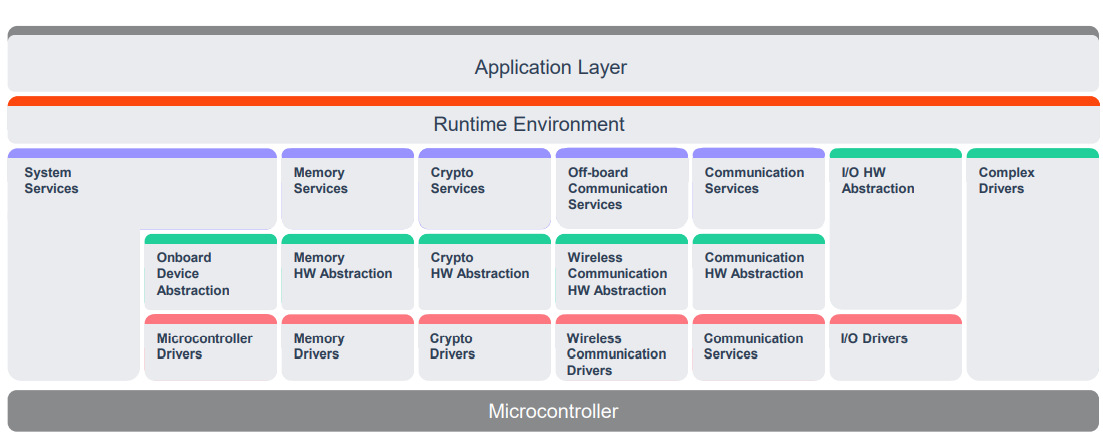
\includegraphics[width=1\textwidth]{imagens/classic platform.png}
  \captionsetup{justification=centering}
  \captionfont{\small{\textbf{\\Fonte: \cite{AUTOSAR}}}}  
  \label{fig:autoclassic}
\end{figure}


\begin{figure}[H]
  \setlength{\abovecaptionskip}{0pt} \setlength{\belowcaptionskip}{0pt}
  \caption{AUTOSAR Adaptive Platform}
  \centering
  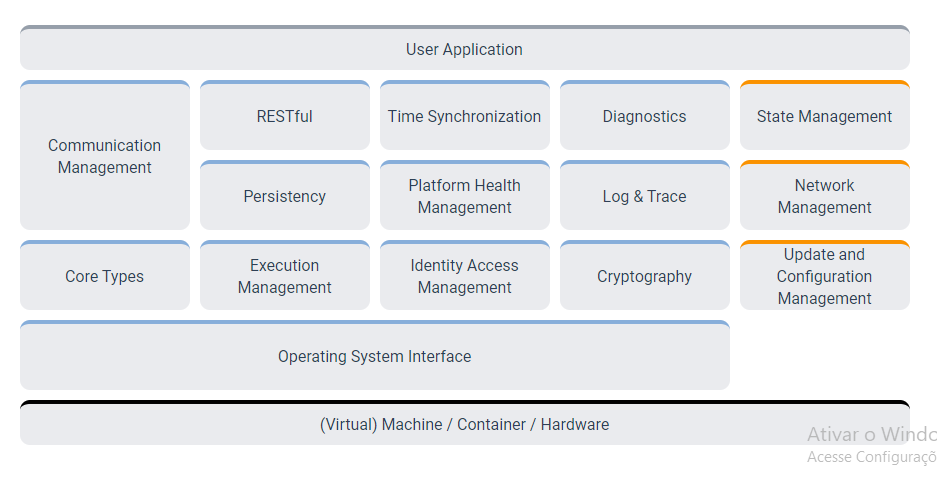
\includegraphics[width=1\textwidth]{imagens/adaptive platform.png}
  \captionsetup{justification=centering}
  \captionfont{\small{\textbf{\\Fonte: \cite{AUTOSAR}}}}  
  \label{fig:autoadaptive}
\end{figure}


\subsection{Robot Operating System}


The Robot Operating System (ROS), despite the name, it was not a operating system in the sense of scheduling and process management but actually a framework to facilitate the development of robotic applications. It needed to run on the top of an operating system providing interface for the users and the machine resources. Developing code for robots was hard due to its size and complexity. The code stack could reach the driver level going up to perception, mapping and reaching the user interface . Also the difference of hardware in each robot could make software reuse impossible without a common developing software \cite{quigley2009}. It was clear that robot development was not a single man task needed a cooperative effort to be developed. These were the main motivations to ROS framework development.

The base of the ROS schema was the Nodes, that were independent software structured in a graph way, remembering the object oriented programming, having some of its advantages. It promoted decoupling and reuse of ROS packages developed by the research community. ROS uses the publish and subscribe fashion for multiple nodes communication and request and response for peer to peer data request. It was able to record and play messages exchanged between nodes using the rosbag feature. It uses the Transmission Control Protocol (TCP) or the User Datagram Protocol (UDP) as a communication tool what enabled the work with distributed system meaning that several computers were seen as one big ROS system independently where the communication nodes are located \cite{ROS}. Furthermore, it was programmed using mostly C++ and Python programming languages.

\begin{figure}[H]
  \setlength{\abovecaptionskip}{0pt} \setlength{\belowcaptionskip}{0pt}
  \caption{Publish Subscriber Schema in ROS Nodes}
  \centering
  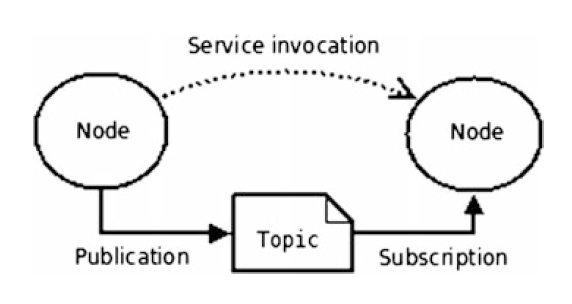
\includegraphics[width=1\textwidth]{imagens/ROSNodes.png}
  \captionsetup{justification=centering}
  \captionfont{\small{\textbf{\\Fonte: \cite{guettier2016}}}}  
  \label{fig:autonodes}
\end{figure}


Looking into the literature, ROS was the most used framework to develop robotic applications being the others frameworks such as AUTOSAR or Apollo based on that. However, when ROS was applied to the ADV, what could be called a special type of ROBOT, it was found some drawbacks. The ADV software system needed to have correct real time responses within a strict time window. Usually the overall system response could no be over 200 milliseconds. Using the TCP or UDP protocol could not guarantee real time response or correctness of the data transmitted through the communication channel what could be catastrophic. 

Furthermore, Valigi, N. \cite{valigi2018} cited some other challenges in developing autonomous vehicle software in ROS. The publish/subscribe pattern is the main issue bringing challenges even in a small scale projects. Inter process communication overhead without a shared memory, performance and reliability through multiple nodes communication over several machines, unnecessary coupling between framework and OS due to many OS-level processes created and the distributed programming mindset necessary even when its not the case were the main drawbacks pointed by the author. Liu et al \cite{Liu2019} also state that reliability as ROS did not monitore its nodes health and the unnecessary duplication of sended messages were issues that degraded the performance  The ROS community organized and developed the ROS 2 to face some of theses challenges. 

The main change in the ROS 2 was the implementation of the Data Distribution Protocol (DDS) substituting the TCP/UDP protocols. The DDS offers the advantage of a real-time data transmission support. Users could prioritize their threads and nodes without the need of a ROS Master thus reducing communication overhead \cite{stavrinos2021}. Another important improvement was the determinism of the execution order of the nodes that was not possible in ROS. ROS 2 was in development \cite{ROS} and even though it brought great improvements in the communication stack with DDS it still hold limitations. Specially the necessity to have a OS like Linux on top of it makes impossible to the whole system to have hard real time behaviour what was necessary for an ADV software system \cite{gutierrez2018} \cite{Reke2020}.

\subsection{Appolo Auto}
Apollo was an open source project from the chinese giant technology company Baidu that atracted several companies as partners. They aimed to provide an ADV software platform, sugested ADV hardware and simulation software with real data to test. Beginning the research in 2013, it was first tested in 2015 and became open for the community in 2017. \cite{Zhang2018} It started in the early versions as an extension of ROS. From the version 3.5 it was replaced by the Cyber RT framework that claimed to be more efficient than ROS itself using a lighter communication structure. Apollo provided many ADV necessary resources such as obstacle perception, route planning, cloud communication and HD maps \cite{Kessler2019} \cite{Liu2017}. 

\begin{figure}[H]
  \setlength{\abovecaptionskip}{0pt} \setlength{\belowcaptionskip}{0pt}
  \caption{Apollo System}
  \centering
  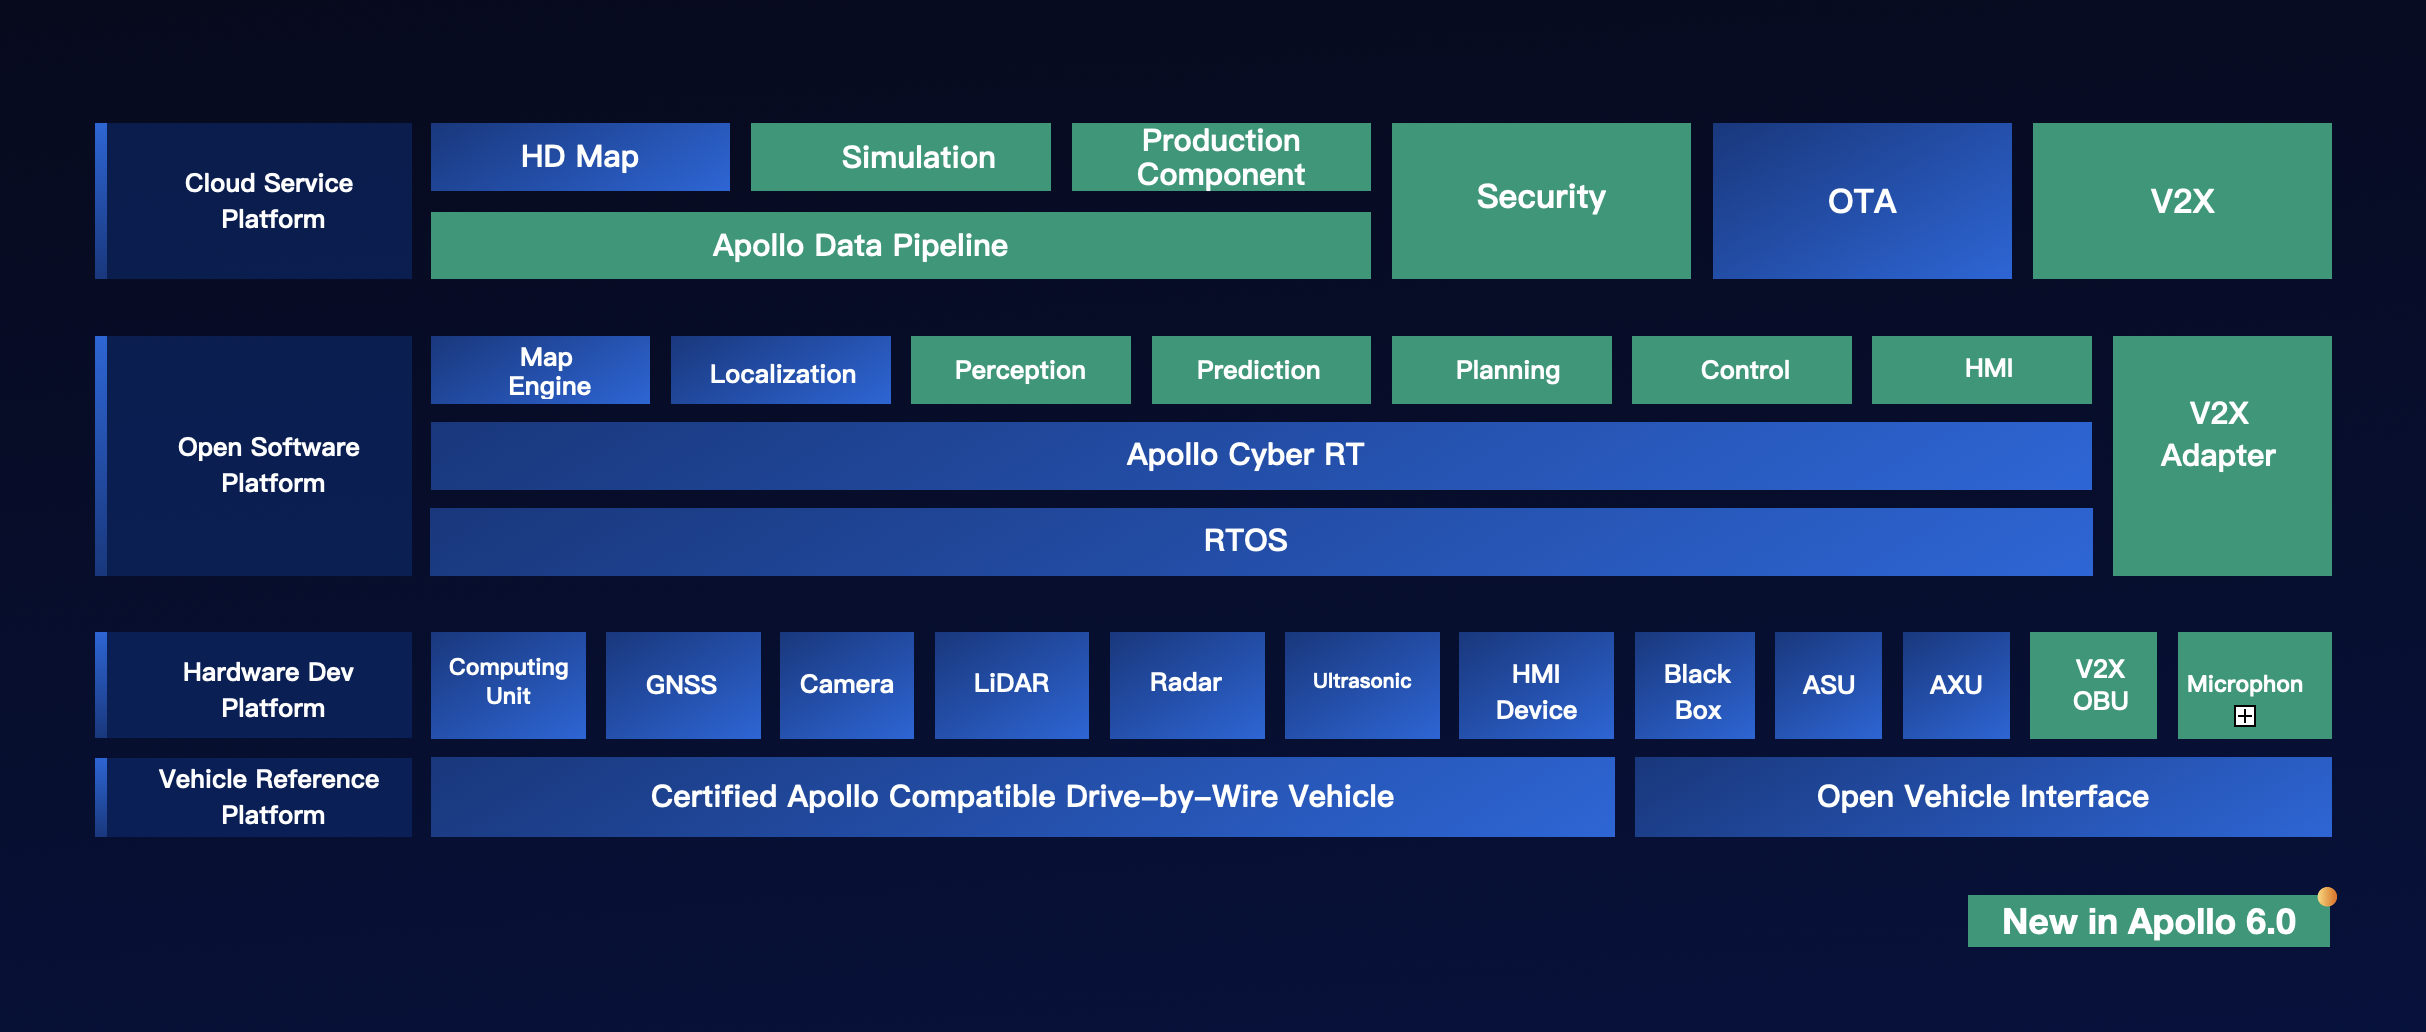
\includegraphics[width=1\textwidth]{imagens/Apollo_6_0.png}
  \captionsetup{justification=centering}
  \captionfont{\small{\textbf{\\Fonte: \cite{ApolloAuto}}}}  
  \label{fig:Apollo}
\end{figure}

The Apollo Kernel was a Linux modified kernel to run the Apollo software stack. It had real time capabilities and latest communication driver. At that time Apollo had already moved from development do productization wit many real applications in the world. Cyber RT was the Apollo framework designed specifically for ADV hardware and logic control. It was developed for a centralized computing architecture and built upon the concept of components\cite{Apollo}. It aimed to improve latency, concurrency and throughput in addition to accelerated development and accelerated deployment. The main innovation comparing to ROS was the possibility to use the RAM memory to transfer messages between modules. It was crucial for transferring messages with a lot of data without delays \cite{Buyval2019}.

Buyval et al. \cite{Buyval2019} found difficulties to use Apollo software, especially the path planning system. It used a multilevel approach with the data fed straight to the controller module. Between the disadvantages presented, the most relevant is that it took too long to process the trajectory. This made it impossible to be applied in a dynamic road scenario. Kessler at al. \cite{Kessler2019} needed to change drivers, include adapters and modify modules to apply the Apollo system in its ADV prototype. The author concludes that many barriers were encountered to use the Apollo System. 

\subsection{NVIDIA DRIVE}\label{ref:ml}

NVIDIA DRIVE was the proprietary solution designed by NVIDIA to control its ADV specific hardware. It was a software stack composed by a RTOS, middleware and software components directed to provide the ADV its necessary resources. It was part of the NVIDIA DRIVE System composed by simulators, software, training platform and was compatible with NVIDIA in-vehicle computers DRIVE AGX and DRIVE PX2. It aimed to deliver a safe and secure execution environment for hard real time applications with secure boot and services, firewall and over-the-air updates.


\begin{figure}[H]
  \setlength{\abovecaptionskip}{0pt} \setlength{\belowcaptionskip}{0pt}
  \caption{NVIDIA DRIVE system}
  \centering
  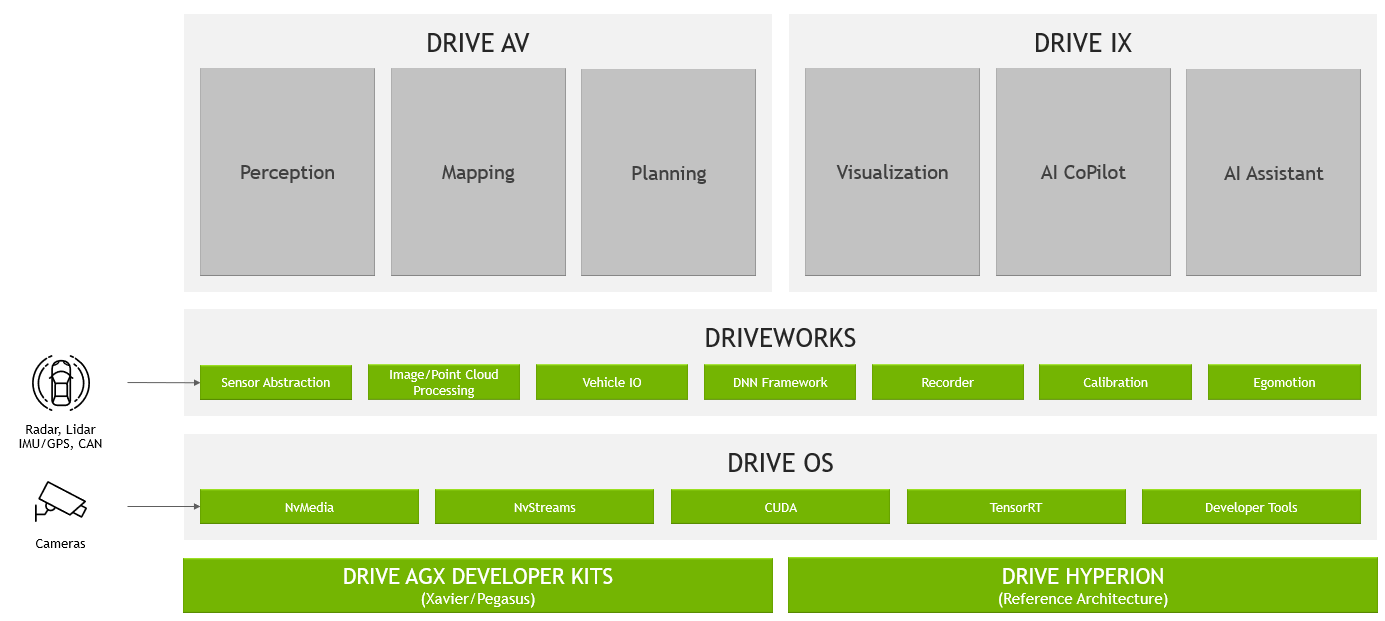
\includegraphics[width=1\textwidth]{imagens/driveworks.png}
  \captionsetup{justification=centering}
  \captionfont{\small{\textbf{\\Fonte: \cite{NvidiaDrive}}}}  
  \label{fig:NvidiaDRive}
\end{figure}

The NVIDIA DRIVE was divided in four parts. The DRIVE OS was the operating system of the stack that provided direct access to the hardware resources. It had a hard real time operating system embedded with the NVIDIA CUDA and TensorRT libraries. It also had a NVIDIA developed Hypervisor for guesting operating systems like Linux versions that provided access to the DRIVE OS itself. The NVIDIA DriveWorks was the midlleware that provided all the necessary libraries modules for ADV specific applications. It dealt with tasks such as sensor signals collection, image and point cloud processing, deep neural networks models and Vehicle IO collection. This middleware ready made components had the objective to use the maximum throughput available on the NVIDIA hardware in use.

On the top of the stack, the DRIVE AV provided the algorithms and strategies for perception, mapping and planning in separated modules. It was accessed using the DRIVE WORKS development interface. It module had an extensive list of resources treated as a separated software component. The last part of the system was the DRIVE IX. It supplied human machine interface and specific features aimed to the interaction with the driver on the vehicle cabinet. It enabled the development of applications such as driver conditions aid, system visualization, voice and face recognition

Researchers have proposed various approaches to optimize task scheduling, including middleware solutions that facilitate data transmission and process management, intelligent scheduling algorithms that dynamically allocate resources, and AI-based strategies that use machine learning for enhanced adaptability and efficiency. This section provides an overview of the existing literature on task scheduling for autonomous vehicles, focusing on both traditional scheduling frameworks and AI-driven techniques.
\subsection{Task Scheduling for Autonomous Vehicles}

The Cocktail Project \cite{Zong2018} was designed to overcome the drawbacks of ROS when dealing with real-time systems. It is a general purpose middleware focused on data transmission. It is used to control communications between the many processes running in an ADV system. It deals with the data as binary streams that are free from any data format of the processes peers. In this project, an intelligent task scheduler called IoThreadPool was introduced. When the IO data from the ADV sensors are collected, this scheduler decides on the best strategy. It could be creating new threads or using threads already available. It also assigns the best available processor to the thread to maximize throughput.

PI-Edge \cite{tang2018} is a computing framework designed to efficiently handle multiple tasks in autonomous heterogeneous computing systems. It was composed of a runtime layer with a scheduler developed in OpenCL. Dynamically dispatches incoming tasks to the best suitable processing unit available. It consists of two layers. The intercore scheduler is the first barrier that receives incoming tasks and assigns them to the computing units based on availability and task affinity. It uses a variation of the Min-Min algorithm developed by the author called Dif-Min. It could obtain an average 10\% reduction in makespan compared to the Min-Min algorithm. The inner-core scheduler organizes the tasks queue inside the same processor based on task priority and dependency between them. It uses the table-based heterogeneous earliest finish time as a scheduling algorithm.

\cite{amarnath2021}  proposed a two level scheduler called HetSched. One level named Meta-Sched processes the DAG dependencies. Verifies if a task is ready to be executed if there is no parent task to be executed on the graph. It also elects DAGs to not be executed due to the unfeasible deadlines of its tasks.  The ready tasks are handled by the Task-Sched that actually delivers tasks to the processing units that can process it. The scheduler ranked the tasks to be executed using its earliest finish time. It was calculated using its execution time, processing unit status, and the task queue scheduled to the same processing unit. The scheduler was tested on a Jetson TX1 board composed of GPU accelerators and CPU processors. The tasks used to test were from two benchmark suites that simulate a simplified autonomous vehicle. Based on the experimental results, it was possible to determine the best configuration of computing units for urban scenarios based on the experimentation.

\subsection{AI-Based Task Scheduling for ADVs}

\cite{Balasekaran2021}  proposed an intelligent task management system for autonomous driving. It was composed of a resource predictor using a single-layer feedforward neural network and a scheduler using the hyper period first algorithm. It was developed in Python and tested on a multicore system consisting of an Odroid XU4 and NVIDIA Jetson embedded platforms. When put against the Connected Autonomous Vehicles and Internet of Medical Things benchmarks it achieved 98\% better accuracy, reduction between 20\% to 27\% of execution time and 32\% to 45\% reduction in task miss rate compared with conventional task scheduling methods.

Furthermore, Xu et al. \cite{Xu2022} propose the Age of Information (AoI)-centric task scheduling approach that aims to ensure that tasks use the most recent sensor data, which is critical for correct detection, planning, and action taking by ADV. The schedule uses a reinforcement learning solution by integrating its scheduler with a DDQN to solve hard combinatorial problems. 

Many recent researches believe that autonomous vehicles would not be able to handle all the computational load required to drive autonomously due to their limited computational resources \cite{qi2020, dai2019, lin2019, liu2019task}. Hence, the use of mobile edge computing servers (MECS) would be necessary to unload autonomous driving tasks from the ADV to the servers. This assumption would become feasible with the 5G network deployment. Therefore, to take advantage of the available edge computing infrastructure, it is necessary to gracefully schedule ADV tasks based on its priorities and characteristics to the most suitable and available MECS. 

Inquiring that the full system, composed of ADV and MECS interconnected by a wireless network, could not be mathematically modeled accurately, \cite{qi2020,liu2019task} proposed the use of a DRL approach to distribute the incoming ADV tasks to the MECSs in a parallel fashion. A set of characteristics from the task are extracted and used as a input for the DRL algorithm that after some training epochs starts to deliver the optimal solution for scheduling the task to the available nodes. Both authors compared their results with well-known scheduling algorithms for heterogeneous computing systems that proved to bring some average processing time reduction to the ADV computing system.

Organizing and scheduling real time tasks responsible for the ADV action-taking process was the objective of \cite{lin2019}. Hence, a reinforcement learning algorithm based on simulated annealing (SA-RL) was proposed to improve system performance. The authors suppose that the tasks would be transferred to edge computing nodes instead of being processed inside the vehicle computing system. The scheduler was designed according to the difference in tasks and sub tasks and changes in the edge computing environment. The problem was described using a Markov decision process, and the completion time was calculated using an algorithm devised by the author. Afterward, a Q-learning algorithm based on simulated annealing was applied to improve the task completion rate. Finally, the proposed SA-RL algorithm was simulated on a computer with a Windows 10 operating system against the particle swarm optimization algorithm. Both algorithms performed well in feasibility and effectiveness; however, the authors' strategy converged faster and maintained a low level of fluctuation with respect to the average completion time.


\end{comment}

%\include{texto/2.2-arquiteturas}
%\chapter{Methodology} \label{metodologia}
\vspace{-1.9cm}

This chapter details the methodology employed to develop, implement, and evaluate the smart task scheduling strategy for heterogeneous Autonomous Driving Vehicles (ADV) processing systems. To provide a structured and comprehensive overview of the research design, the methodology is divided into the following main stages:

\begin{itemize}
    \item \textbf{Material:} Description of the software, frameworks, and hardware infrastructure utilized to build the simulation and scheduling environment.
    \item \textbf{Setup of the Test Environment:} The integration of the ADV simulator with the task scheduling framework.
    \item \textbf{Design of the ADV Smart Task Scheduling Strategy:} The modeling of the ADV computational workload and the proposed scheduling approach.
    \item \textbf{Implementation and Testing:} The practical application of the proposed strategy within the simulated environment.
    \item \textbf{Results Analysis and Evaluation:} The metrics and benchmarks used to assess the performance of the proposed scheduling algorithm.
\end{itemize}

\section{Material} \label{sec:material}

To develop and evaluate the novel task scheduling strategy, a specific set of tools, frameworks, and hardware components was selected to accurately simulate the computational demands of an Autonomous Driving Vehicle (ADV). This section describes the primary components that comprise the testbed infrastructure.

\subsection{Simulation Platform}
The CARLA (Car Learning to Act) simulator \cite{Dosovitskiy17} was employed as the primary open-source platform to replicate real-world autonomous driving scenarios. CARLA was selected due to its high-fidelity rendering, realistic urban environments, and robust Python API, which provides extensive flexibility in configuring simulation parameters, controlling vehicle sensors (e.g., cameras, LIDAR, radar), and defining complex traffic scenarios involving varying densities, pedestrian behaviors, and weather conditions. Crucially, CARLA allows for the extraction of sensor data in real-time, functioning as the primary workload generator for the ADV perception pipeline.

\subsection{Task Scheduling Framework}
To manage the computational workload generated by the ADV simulator across a heterogeneous processing architecture, the StarPU runtime system \cite{Augonnet2011} was utilized. StarPU is a task programming library for hybrid architectures that provides a unified execution model. It was chosen for its capability to seamlessly manage task graphs (Directed Acyclic Graphs - DAGs) across different processing units (CPUs and GPUs), its comprehensive set of profiling and tracing tools, and, most importantly for this research, its flexible API that allows users to write and plug in custom scheduling policies \cite{starpuscheduling2024}. 

\subsection{Programming Languages and Libraries}
The core integration between the CARLA simulator and the StarPU runtime was developed using \textbf{C++} and \textbf{Python}. Python was heavily utilized for interacting with the CARLA API and managing the high-level simulation scripts, leveraging its extensive ecosystem for data analysis and machine learning. C++ was employed for performance-critical components, specifically for developing the StarPU application client, defining the StarPU \textit{codelets} (task implementations), and interfacing directly with the StarPU C API to ensure minimal overhead during task submission and scheduling.

For the object detection workload within the ADV perception pipeline, the YOLO (You Only Look Once) architecture was incorporated, utilizing deep learning frameworks to process the camera data streams extracted from CARLA. 

\subsection{Test Environment Hardware}
The experiments and simulations were conducted on a heterogeneous computing platform to evaluate the scheduling strategies under realistic hardware constraints. The test environment was composed of a system equipped with both multi-core Central Processing Units (CPUs) and Graphics Processing Units (GPUs), representing the heterogeneous nature of modern ADV embedded systems. [NOTE TO USER: Please insert the specific hardware details here: e.g., Intel Core i9 processor, 32GB RAM, NVIDIA RTX 3080 GPU, running Ubuntu 22.04 LTS].

%% - Proposta: é sua arquitetura, descrição, etc...
% O que é ser parametrizável? Muitas vezes alguém faz um projeto de descrição de hardware em vhdl para uma NoC 4x4 de forma rígida. Ou seja, se você quiser sintetizar uma NoC 8x8, você vai ter que editar e refazer vários dos vhdls do projeto. É literalmente um reprojeto. 
% Se a descrição fosse parametrizável, haveria um arquivo de variáveis, onde por exemplo, teria uma que diria o tamanho da NoC=4. Você iria lá, alteraria para 8, e não faria mais nada. Ao fazer a nova síntese, o hardware seria 8x8. Ou seja, o projeto foi feito com uso de variáveis/parâmetros para que uma nova síntese não implique em novo projeto de hardware.

\chapter{The Cart-OnePiece Framework Overview} \label{ch:framework}
\vspace{-1.9cm}

\section{System Architecture and Perception Pipeline} \label{sec:system_pipeline}

The Cart-OnePiece framework is structured as a comprehensive environment designed for synthetic dataset generation, Advanced Autonomous Driving (ADV) workload characterization, and the evaluation of custom task scheduling policies. To achieve these goals, the architecture is built around an asynchronous sensor processing pipeline that closely couples the CARLA simulator \cite{Dosovitskiy2017} with the StarPU runtime system and the NVIDIA TensorRT inference engine. This integration allows the extraction of high-frequency sensor data, its computation across heterogeneous resources, and the observation of the system's performance under distinct scheduling constraints.

A high-level overview of the framework's operational pipeline is presented in Figure~\ref{fig:framework_pipeline}. The system operates on a client-server model where the CARLA server acts as the primary workload generator, simulating the physics, traffic, and environmental conditions of the urban scenario while rendering the virtual world from the perspective of the ego-vehicle. On the client side, a C++ application implemented on top of the StarPU library dictates the asynchronous extraction and processing of these sensor streams.

\begin{figure}[hbt!]
  \centering
  
\includegraphics[width=\textwidth]{Figure2.png}
  \caption{Overview of the Cart-OnePiece framework and the autonomous driving perception pipeline.}
  \label{fig:framework_pipeline}
\end{figure}

The core of the execution flows through a continuous perception pipeline composed of consecutive computational stages. In the initial phase, multiple virtual cameras attached to the simulated vehicle output raw visual data (typically in RGBA format) and their corresponding semantic segmentation ground truth. Rather than blocking the main execution thread to process these images immediately, the StarPU runtime is tasked with managing these operations asynchronously, mapping them dynamically to the available CPU workers and GPU resources.

Once the raw data is captured, a preprocessing stage converts the images from the simulator's native BGRA format into the NCHW tensor layout required by deep learning engines, normalizing the pixel values simultaneously. This stage is highly parallelizable and is primarily distributed among the host CPU cores. Following the preprocessing, the normalized tensors are dispatched to the inference stage. Here, the TensorRT library, accelerated via CUDA, processes the data using pre-compiled models, such as ResNet50 or DeepLabV3, predicting the semantic masks of the scene.

The resulting semantic predictions are then evaluated against the synchronously captured ground truth in a metric calculation stage, which computes the Mean Intersection over Union (mIoU) and pixel accuracy. To ensure that the computational trace is accurately registered without interfering with the workload execution, the pipeline relies on the APEX profiling tool and StarPU's internal FxT tracing mechanisms, which record the latency, memory utilization, and structural task dependencies of each frame.

This architectural design not only provides a flexible testbed for characterizing the ADV workload but also exposes a mechanism to control the depth of in-flight tasks and constrain resource mappings. By keeping the different processing stages decoupled through the StarPU runtime, the Cart-OnePiece framework enables a direct evaluation of how different scheduling policies impact the end-to-end latency and the efficiency of heterogeneous component utilization.



\chapter{Conclusion} \label{conclusoes}
\vspace{-1.9cm}

The advancement of autonomous driving vehicles has immense potential to revolutionize transportation by improving safety, efficiency, and accessibility. However, the complexity of integrating sophisticated software algorithms with heterogeneous hardware systems presents significant challenges. Traditional task scheduling methods, designed primarily for homogeneous or single-core processors, are insufficient for managing the diverse computational demands of modern ADVs. 

This thesis proposal aims to develop a smart task scheduling strategy for heterogeneous processing platforms in autonomous vehicles, with a focus on improving system performance, reducing energy consumption, and achieving safe driving suitable for commercial deployment. By modeling the ADV's computational tasks as a directed acyclic graph and employing a reinforcement learning algorithm for scheduling decisions, the proposed approach aims to dynamically learn and adapt to system behaviors. 

The methodology involved the creation of an integrated test environment that combines the CARLA simulator with the StarPU runtime system. This setup enables realistic simulation of ADV scenarios and provides a platform to implement and evaluate the proposed scheduling strategy. By utilizing StarPU's feature to define custom scheduling policies, the reinforcement learning model can be smoothly integrated into the simulation environment, allowing for dynamic task placement and resource allocation across CPUs and GPUs. Preliminary results showed the feasibility of this integration with the application of different scheduling strategies prefedined in the StarPU runtime system directly into the CARLA simulation.

The next chapter shows the schedule with a brief explanation of the work in development and the next steps to complete the development of the proposed smart task scheduling strategy.


\chapter{Schedule and Future Work}
 \label{schedule}
\vspace{-1.9cm}

The detailed timeline of activities is presented in Figure \ref{fig:sched}, which shows the planned progression over each month.

\begin{figure}[ht]
  \centering
  
  % Caption setup for this specific figure
  \captionsetup{
     labelfont={bf,large},       % label (e.g., "Figure 1:") in bold and large
     textfont={bf,large},        % caption text in bold and large
     justification=raggedright,  % left-align the caption
     singlelinecheck=off         % force left alignment even for short captions
  }
  
  \caption{\MakeUppercase{Thesis Schedule}}
  \label{fig:sched}
  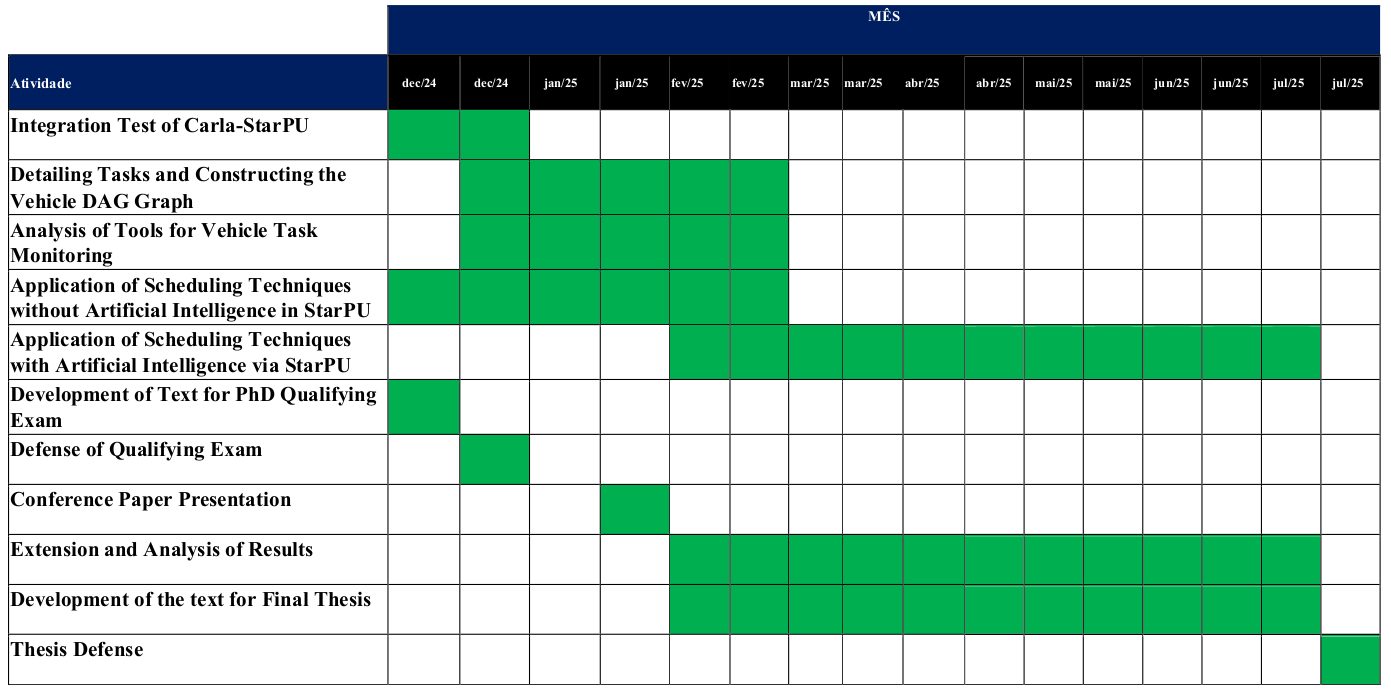
\includegraphics[width=\textwidth, keepaspectratio]{imagens/QualiExt.png}
\captionfont{\small{\textbf{\\Source: Created by the Author}}} 
\end{figure}

The work in progress from Steps 1 to 4 generated the conference paper in Appendix \ref{anexo-accepted} to be present in January 2025. This work is still in progress to consolidate the basic setup using predefined StarPU scheduling strategies. Upon completion of these steps the objective is to start to develop and test the novel scheduling collecting and validating results for the Thesis. The author expects from these results to elaborate one paper submission showing the community the new scheduling method for Autonomous Driving Vehicles. The end of this work is planned to happen by July 2025, however, the intention is to finish the Thesis a couple of months earlier as soon as the development and results are consolidated.

%\include{texto/8conclusao}
% O * no include faz com que o texto do arquivo seja incluído na mesma página, e não na próxima. O setboolean evita isso também, evitando que o texto incluído vá para o anverso.
%\setboolean{@openright}{false}
%\include*{texto/5resultadosA}
%\include*{texto/5resultadosB}
%\include*{texto/5resultadosC}
%\setboolean{@openright}{true}

%%%%%%%%%%%%%%%%%%%%%%%%%%%% PÓS-TEXTUAIS %%%%%%%%%%%%%%%%%%%%%%%%%%
% Bibliografia no arquivo 'Dissertacao.bib'
% Alterar o título das referências para somente 'Referências'
%%%%%%%%%%%% NÃO SE ESQUEÇA DE ACERTAR AS REFERÊNCIAS!!! %%%%%%%%%%%%
\renewcommand{\bibname}{Referências}
\bibliographystyle{include/abnt-alf}
\bibliography{ref}

% Para forçar que os apêndices e anexos comecem no anverso
%\setboolean{@openright}{true}
\setboolean{@twoside}{false}

%\apendice
%\begin{apendice}
%\include{pos-texto/questionario}
%\end{apendice}
\appendix
% Nome do Anexo
\chapter{Published Paper}
\vspace{-1.9cm}

Article entitled \textbf{A Systematic Mapping of Autonomous Vehicle Prototypes: Trends and Opportunities}, published in \textbf{IEEE Transactions on Intelligent Vehicles} in 2023.

The paper discusses the evolution of autonomous driving vehicles (ADVs) and aims to identify trends and opportunities in the development of these prototypes. Using a systematic mapping study, the paper analyzes 68 selected publications from a set of 548 papers. It provides insights into the hardware, software, and sensor architectures used in both real-size and miniature ADV prototypes. The mapping identifies key trends, technologies, and research opportunities, aiming to support researchers and developers in designing efficient ADVs.

\includepdf[pages=-, pagecommand={}]{pos-texto/IEEE_TIV.pdf}

% Nome do Anexo
\chapter{Published Paper}
\vspace{-1.9cm}

Article entitled \textbf{Hierarchical Heterogeneous Cluster Systems for Scalable Distributed Deep Learning}, published in \textbf{2024 IEEE 27th International Symposium on Real-Time Distributed Computing (ISORC)} in 2024.

Distributed deep learning framework tools should aim at high efficiency of training and inference of distributed exascale deep learning algorithms. There are three major challenges in this endeavor: scalability, adaptivity and efficiency. Any future framework will need to be adaptively utilized for a variety of heterogeneous hardware and network environments and will thus be required to be capable of scaling from single compute node up to large clusters. Further, it should be efficiently integrated into popular frameworks such as TensorFlow, PyTorch, etc. This paper proposes a dynamically hybrid (hierarchy) distribution structure for distributed deep learning, taking advantage of flexible synchronization on both centralized and decentralized architectures, implementing multi-level fine-grain parallelism on distributed platforms. It is scalable as the number of compute nodes increases, and can also adapt to various compute abilities, memory structures and communication costs.

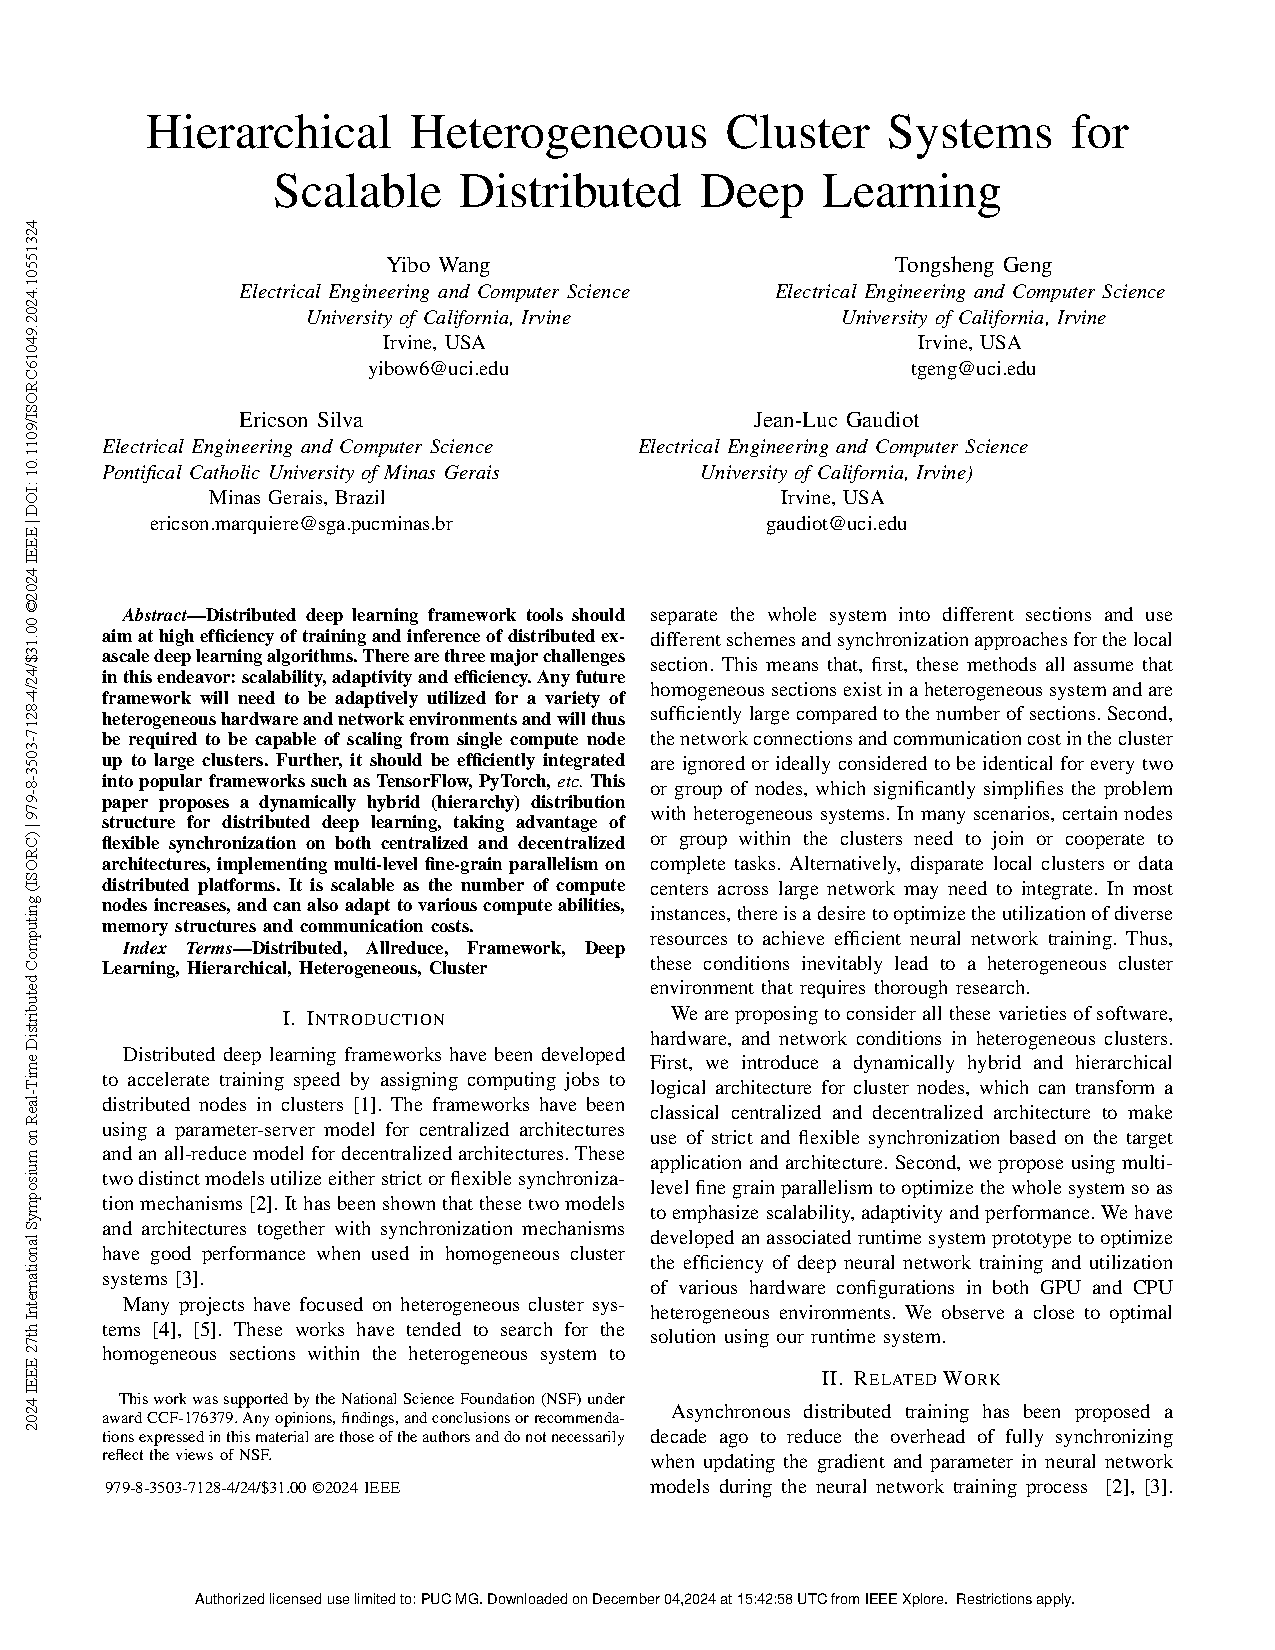
\includepdf[pages=-, pagecommand={}]{pos-texto/IEEE_ISORC}

\chapter{Accepted Paper}
\label{anexo-accepted}
\vspace{-1.9cm}

Article entitled \textbf{Task Scheduling for Autonomous Vehicles with Heterogeneous Processing via Integration of the CARLA Simulator and StarPU Runtime},accepted for publication in \textbf{IEEE International Conference on Consumer Electronics (ICCE)}, with a presentation scheduled for January, 2025.

The paper presents an innovative approach that integrates the CARLA simulator with the StarPU runtime system to optimize task scheduling in autonomous driving vehicles. By combining CARLA's detailed simulation capabilities with StarPU's flexible task management, the study explores efficient scheduling strategies for ADV perception and localization tasks using heterogeneous processing resources (CPU and GPU). The results indicate improvements in ADV performance, demonstrating the practicality of this integration for testing and optimizing task scheduling in realistic simulation environments.

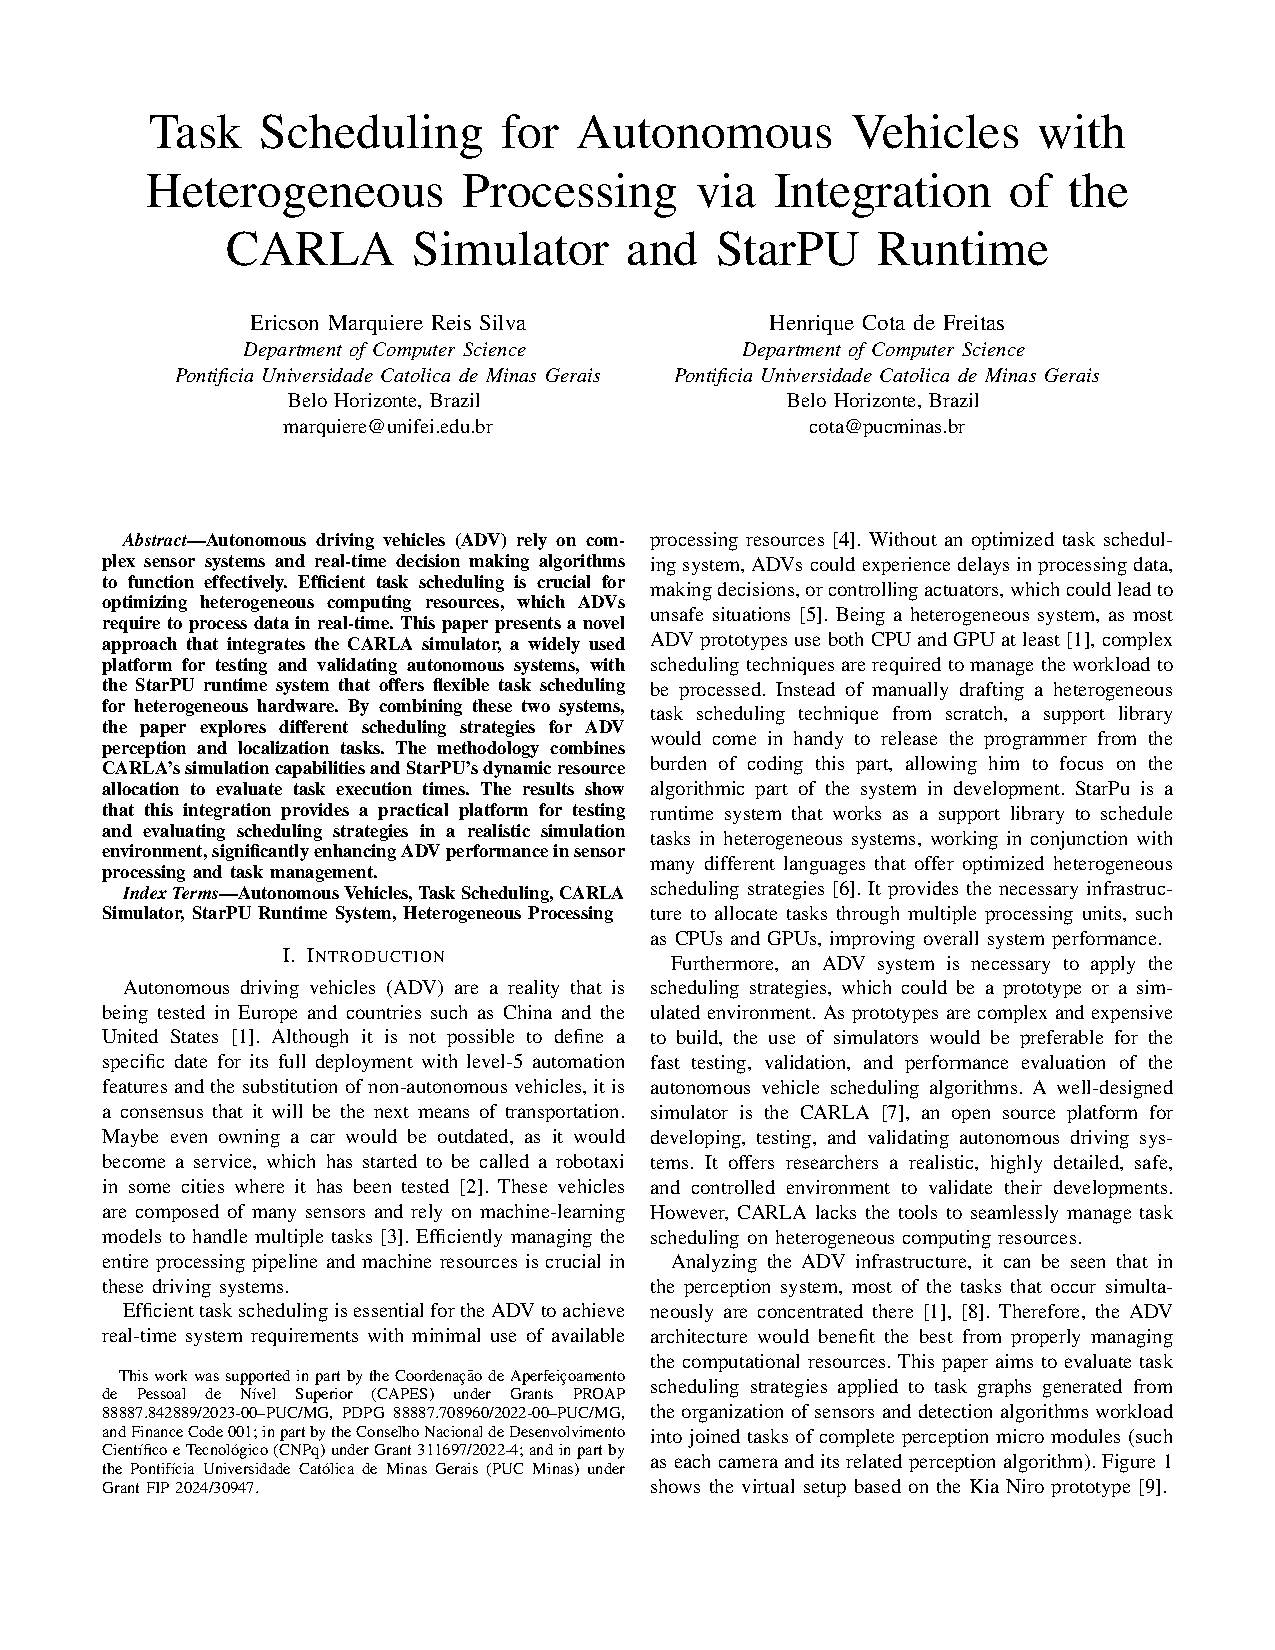
\includepdf[pages=-, pagecommand={}]{pos-texto/IEEE_ICCE.pdf}




\end{document}
